\documentclass[footheight=20pt, footsepline, headheight=20pt, headsepline]{book}
%
\usepackage[utf8]{inputenc} % below are various important packages
%\usepackage{lmodern}
%\usepackage[T1]{fontenc}
%\usepackage[english]{babel}
%\usepackage{textcomp} 
\usepackage{amsmath}
%\usepackage{mathrsfs}
%\usepackage{latexsym}
\usepackage{amssymb}	
\usepackage{amsfonts}
\usepackage{theorem}
\usepackage{graphicx}
\usepackage{eso-pic}
\usepackage{tikz}
\usepackage{scrlayer-scrpage}
\usepackage{xcolor}
\usepackage{setspace}
\usepackage{framed}
\usepackage{hyperref}
\usepackage{relsize}
%\usepackage{pgf,tikz,pgfplots} % possibility to insert geogebra graphs
%\usepackage{mathrsfs}
%\pgfplotsset{compat=1.15}\usetikzlibrary{arrows} % part of geogebra package
%\usepackage{qrcode} % insert qr codes
%\usepackage{multicol}
%\usepackage{multirow}
%\usepackage{xurl}
%\usepackage{tabularx}
%\usepackage{enumitem}
\usepackage{float}
%\usepackage{colortbl,rotating,booktabs} % required packages for Excel2Latex
\usepackage{wrapfig}
\usepackage{listings}
\usepackage[backend=biber]{biblatex}
\addbibresource{bibliography.bib} %Import the bibliography file

\definecolor{codegreen}{rgb}{0,0.6,0}
\definecolor{codegray}{rgb}{0.5,0.5,0.5}
\definecolor{codepurple}{rgb}{0.58,0,0.82}
\definecolor{backcolour}{rgb}{0.95,0.95,0.92}

\lstdefinestyle{mystyle}{
    backgroundcolor=\color{backcolour},   
    commentstyle=\color{codegreen},
    keywordstyle=\color{magenta},
    numberstyle=\tiny\color{codegray},
    stringstyle=\color{codepurple},
    basicstyle=\ttfamily\footnotesize,
    breakatwhitespace=false,         
    breaklines=true,                 
    captionpos=b,                    
    keepspaces=true,                 
    numbers=left,                    
    numbersep=5pt,                  
    showspaces=false,                
    showstringspaces=false,
    showtabs=false,                  
    tabsize=2
}
\lstset{style=mystyle}


% Add to length for wider margins
\addtolength{\textwidth}{3cm} % right to margin
\addtolength{\hoffset}{-1.6cm} % left to margin
\addtolength{\voffset}{-2cm} % to top
\addtolength{\textheight}{4cm} % to bottom

% Headers-Footers
\definecolor{gro}{gray}{0.6} % define color
\setkomafont{pagehead}{\normalfont\sffamily} % define header
\setkomafont{pagefoot}{\normalfont\sffamily} % define footer
\addtokomafont{headsepline}{\color{gro}} % define header horizontal line
\addtokomafont{footsepline}{\color{gro}} % define footer horizontal line
	\ihead{\color{gro} } % header (i=inner=left)
	\chead{\color{gro} } % header (c=center)
	\ohead{\color{gro} \chaptername~ \thesection} % header (o=outer=right)
	\ifoot{\color{gro} } % footer (i=inner=left)
	\cfoot{\color{gro} - {\textbf\thepage} -} % footer (c=center)
	\ofoot{\color{gro} } % footer (o=outer=right)


\renewcommand{\familydefault}{\sfdefault} % font
\linespread{1.2} % increase line spacing

%---------------------------------------------------------------------------
\begin{document} % every document starts with \begin{document}
%\doublespacing

\begingroup
\thispagestyle{empty}
\AddToShipoutPicture*{\put(0,-60){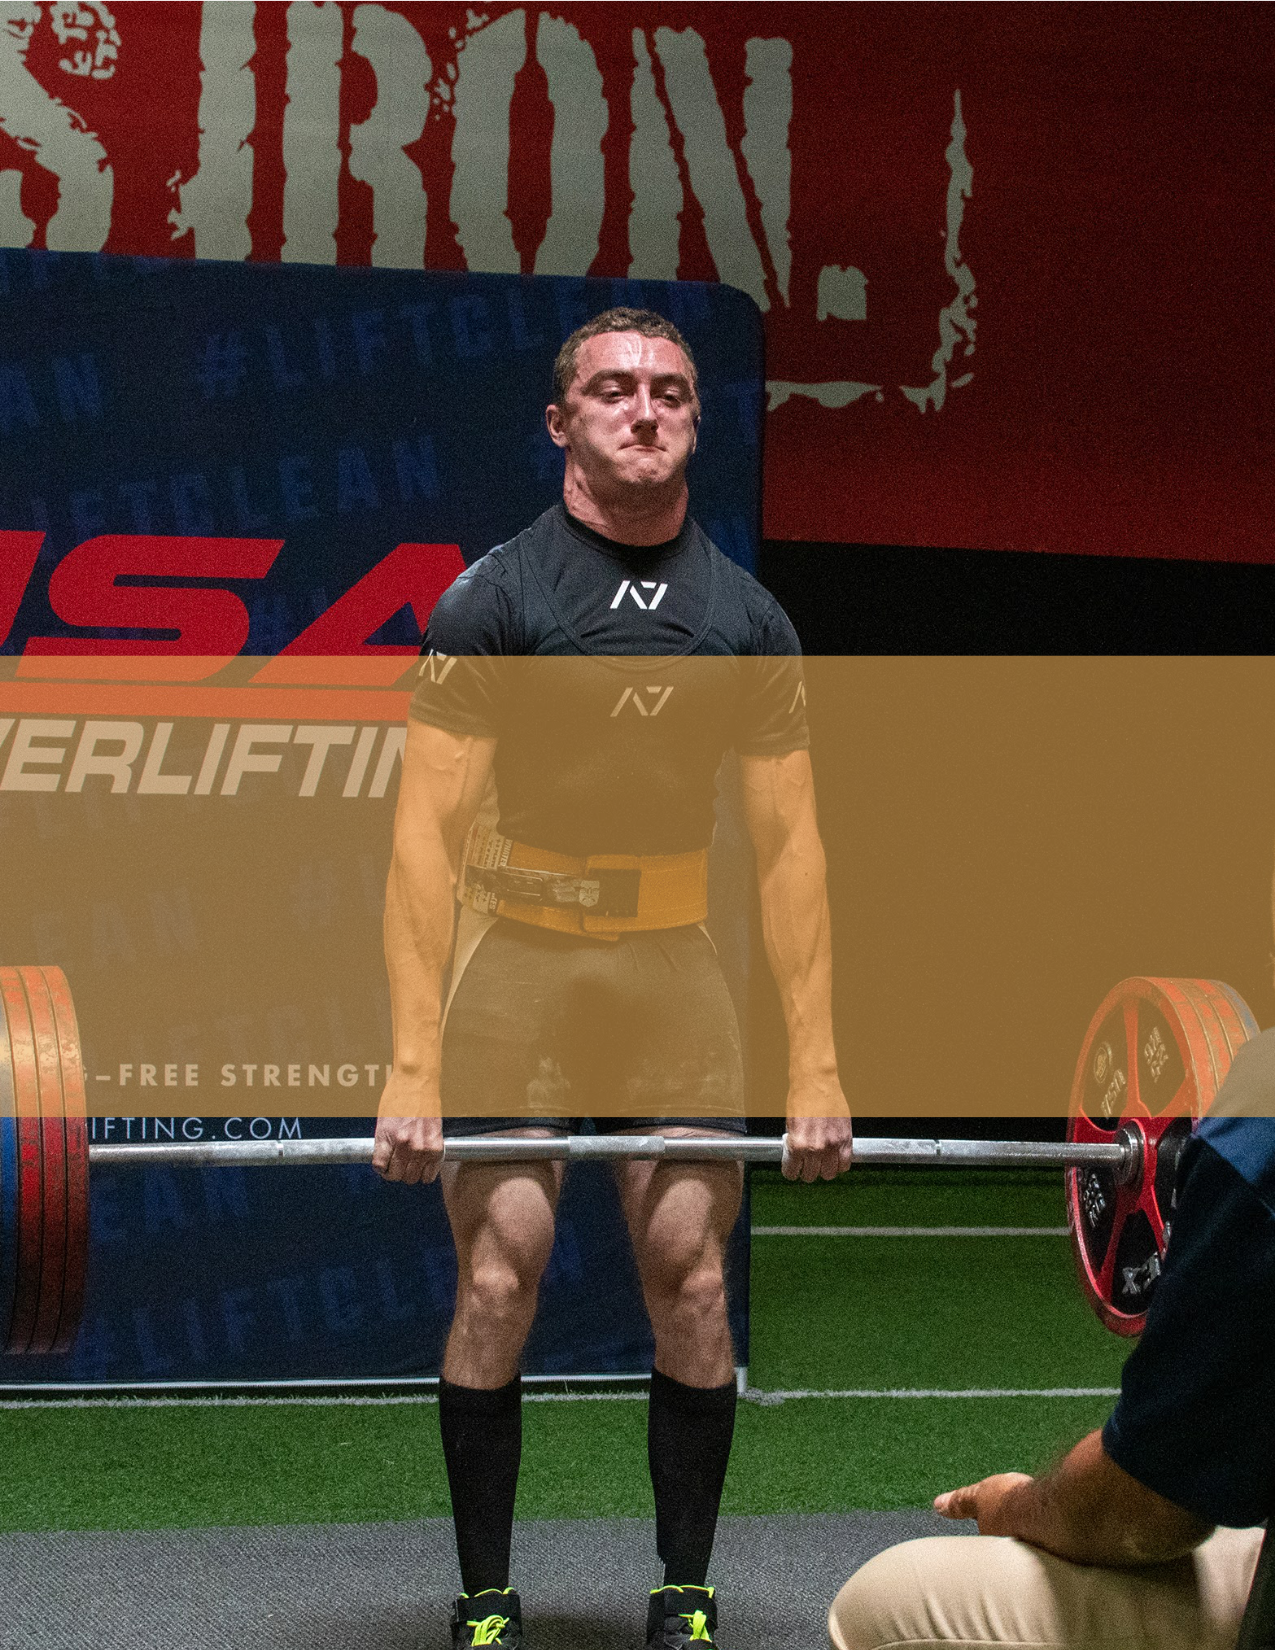
\includegraphics[scale=2.2]{PaperPics/Cover.png}}} % Image background
\centering
\vspace*{8cm}
\par\normalfont\fontsize{35}{35}\sffamily\selectfont
\textbf{Building An Adaptable Training Model}\\
{\LARGE A Mathematical Characterization of a Powerlifting Program}\par % Book title
\vspace*{1cm}
{\Huge Jack Carmichael}\par % Author name
\endgroup

%\AddToShipoutPicture*{\put(0,-60){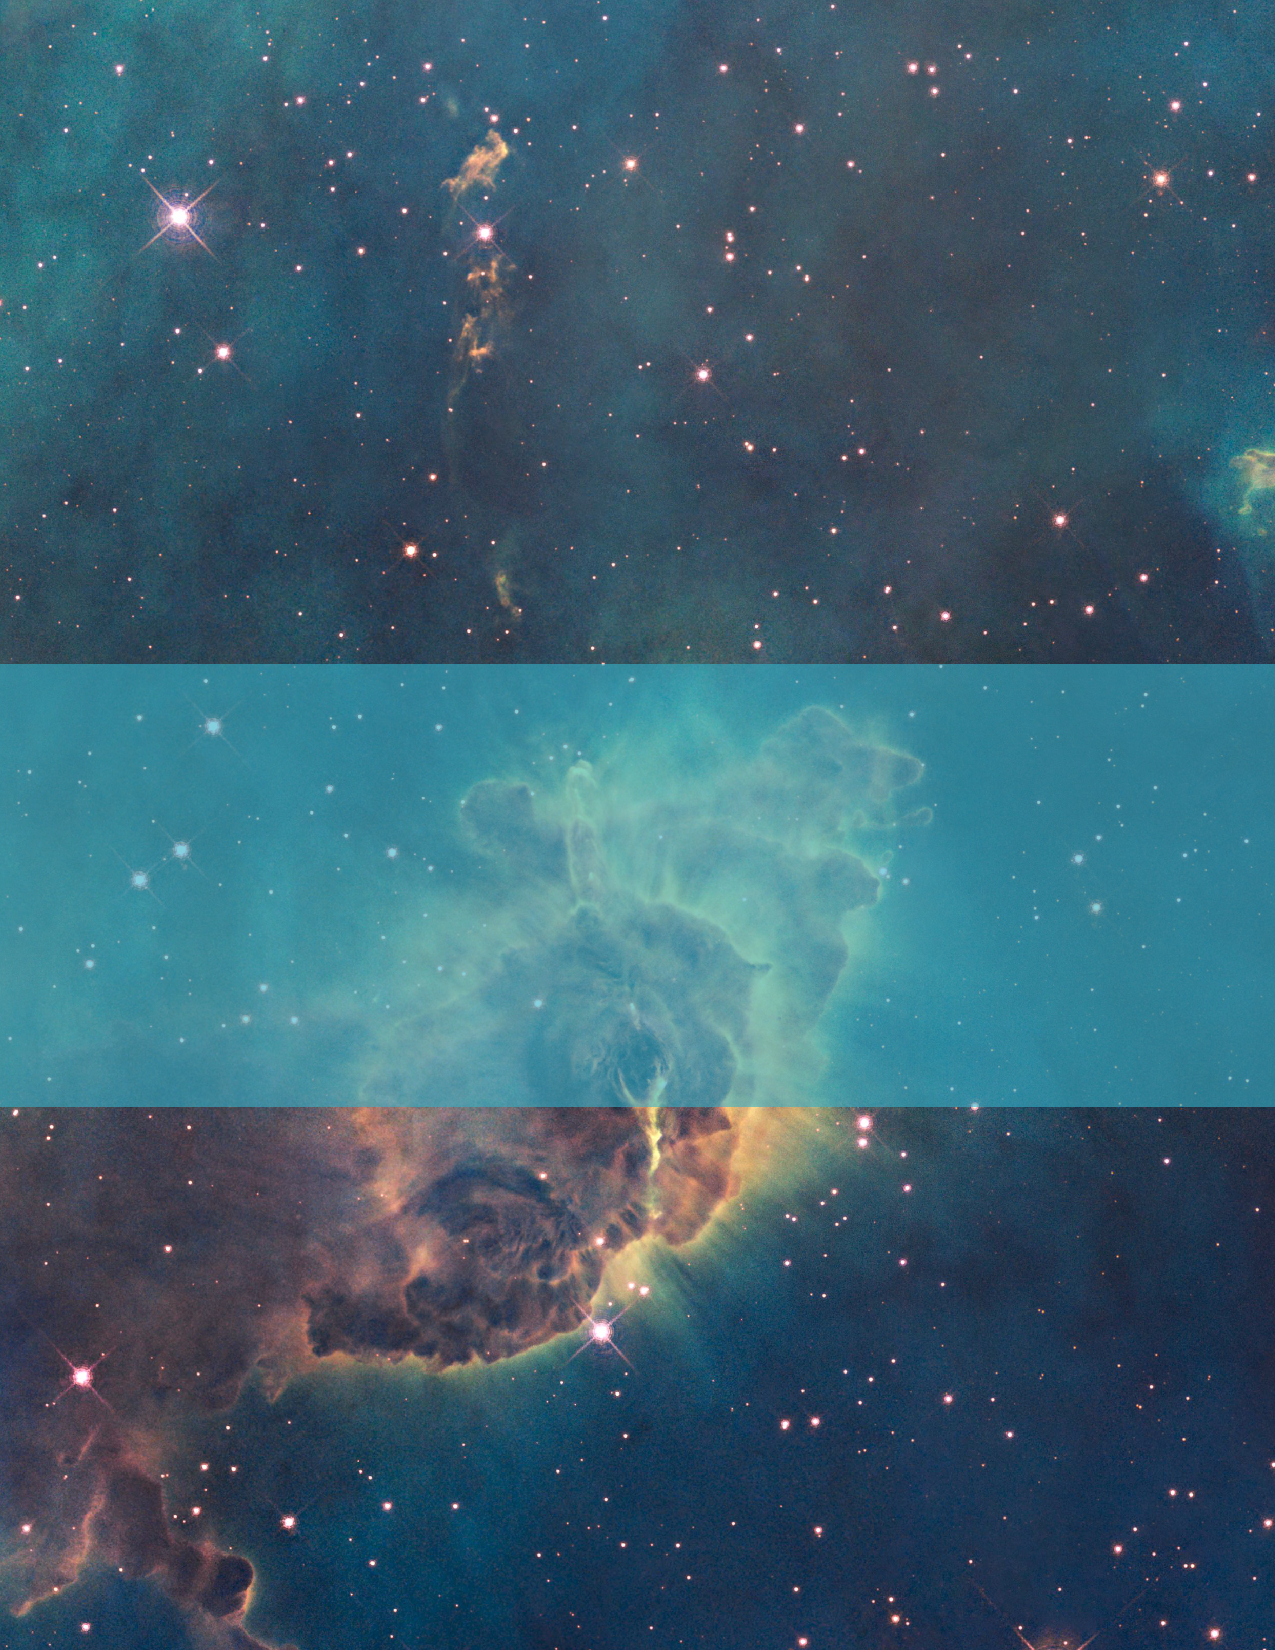
\includegraphics[scale=1.25]{PaperPics/esahubble.png}}} % Image background
% \begingro
% \par
% \normalfont\fontsize{35}{35}\sffamily\selectfont
% \title{\textbf{Building an Adaptable Training Model}\\[1cm]
% Mathematical Characterization of a Powerlifting Program\\[1cm]} 
% \author{Jack Carmichael}
% %\date{\vspace{9cm}\normalsize{\textit{"Besides, it is a disgrace to grow old through sheer carelessness before seeing what manner of man you may become by developing your bodily strength and beauty to their highest limit. But you cannot see that, if you are careless; for it will not come of its own accord."}}\\- Socrates}
% % \date{\vspace{10cm} Colorado School of Mines \\[0.5cm] Mathematics - your class \\[0.5cm] Investigation/IA/EE \\[0.5cm] Word Count: xx}
% \maketitle
%---------------------------------------------------------------------------
\newpage
%~\vfill
\thispagestyle{empty}

\vspace*{\fill}
\textit{"Besides, it is a disgrace to grow old through sheer carelessness before seeing what manner of man you may become by developing your bodily strength and beauty to their highest limit. But you cannot see that, if you are careless; for it will not come of its own accord."}\\
\begin{center}
    - Socrates
\end{center}
\vspace*{\fill}
%---------------------------------------------------------------------------
\newpage
\tableofcontents
%---------------------------------------------------------------------------
\newpage
\part{Introduction}
\label{sec:Introduction}

\chapter{What This Book is and the Basics}

Lots of workout programs exist for powerlifters. Usually these come in the form of a static spreadsheet that do not change, merely presenting the lifer with a template to robotically follow. Even if a workout program does offer some form of adaptability, it is usually extremely limited in scope, capturing only a small portion of the variables that are relevant, and ignoring the fact that not all people respond to training in the same way. For example, some people respond well to high volume and others don't, some people have a lower tolerance to intensity than 'average', and some people cannot perform a certain lift very well due to prior injuries or lack of skill. This lack of adaptability gets even worse when considering that a lifter does not respond to training the same way across time, requiring continual adjustments to achieve maximum potential.

Typically a lifter would hire a coach to manage and adapt there training for them and there current constraints. The goal of this book is to 'dive into' a coaches mindset and mathematically capture ideas fundamental to the jobs they perform. The hope is that the model outlined in this paper will be sufficient to constitute a training program that a lifter can follow and make progress with.

\section{Outline}
\label{sec:Outline}

Below is an outline of what each chapter covers.

\begin{enumerate}
    \setcounter{enumi}{1}
    \item \textbf{Introduction} \\ \textit{Where You Are Now} \\
    		This chapter sets the common ground and defines terms that will be used throughout the rest of this book. If you are familiar with the terminology behind lifting, section \ref{sec:CommonTermsSection} may be skipped, but section \ref{sec:SmallDifferencesSection} can save you from future confusion.
    		
    \item \textbf{Data} \\ \textit{The Source of Truth} \\
        This chapter introduces the data as well as important events that occurred when the data was recorded. The generation and reasoning behind any augmented data is also discussed. While here, units and domains of measurement are discussed to frame future discussions.
        
    \item \textbf{Potential Surface} \\ \textit{Establishing What's Possible} \\
        This chapter is where the modeling begins, and defines what is possible for a lifter to complete. While establishing what is possible, it also introduces novel ways to describe what is happening during training.
        
    \item \textbf{Time Frame} \\ \textit{Fine Tuning The Model} \\
        This chapter is concerned with defining the models state along with how it moves through time to match the changes a lifter is experiencing, allowing the model to adapt to the lifter. While discussing adaptations through time, the models reaction to injuries is also discussed.
\end{enumerate}

\section{Common Terms: Getting on the Same Page}
\label{sec:CommonTermsSection}

Throughout the rest of this book several terms will be used. Because this book is going to be read by people outside of the lifting community, some common concepts and there associated terminology will be introduced here. If you are familiar with lifting and the concepts surrounding training, this section can be skipped.

\subsection{General Terminology}
\label{sec:GeneralTerminology}

A \textit{workout program} consists of a series of \textit{exercises} to complete on a given day. Exercises vary depending on what a lifter's goals are, amongst other factors. Exercises are composed of \textit{sets}. Sets are composed of \textit{reps}, short for repetitions, making a rep the smallest unit of work in the gym. Given this, a workout program is just a list of exercises to complete over time where each exercise has a specific number of sets and reps to be done at a specific weight. Table \ref{tab:WorkoutProgramExample} exemplifies this.

\begin{table}[h]
    \centering
    \begin{tabular}{c|c|c|c|c|c}
        Date & Exercise & Sets & Reps & Weight & Effort \\
        \hline
        Mon, July 4\textsuperscript{th} & Deadlifts & $6$ & $6$ & $405$ lbs & $8.5$ \\
        Mon, July 4\textsuperscript{th} & Barbell Rows & $5$ & $10$ & $135$ lbs & - \\
        Mon, July 4\textsuperscript{th} & Lat Pulldowns & $5$ & $15$ & $120$ lbs & - \\
        Tue, July 5\textsuperscript{th} & Squat & $3$ & $8$ & $345$ lbs & $9$ \\
        Tue, July 5\textsuperscript{th} & Goblet Squats & $5$ & $15$ & $85$ lbs & - \\
        \dots & \dots & \dots & \dots & \dots & \dots \\
    \end{tabular}
    \caption{A table showing how a workout is represented. This data is made up as an example.}
    \label{tab:WorkoutProgramExample}
\end{table}

As shown in table \ref{tab:WorkoutProgramExample}, there is one more descriptive element that will give a more complete picture of what is happening across a workout program: \textit{effort}. Every combination of exercises, sets, reps, and weight will be performed at a particular effort. Effort describes how hard a lifter will need to work to complete the prescribed exercise at the given sets, reps, and weight. Effort is generally only used for \textit{compound movements}, or an exercise that requires more than one joint.

Effort will be measured on a scale known as \textit{rate of perceived exertion}, or \textit{RPE}. After every set, a lifter can rate the amount of effort they feel they exerted according to table \ref{tab:RPETable}. The RPE scale is widely used, well researched, and has been proven to be the best method for a lifter to rate the effort required to complete a lift. \cite{RPE_ACCURACY}

\begin{table}[h]
    \centering
    \begin{tabular}{c|l}
        Effort Rating & Description \\
        \hline
        $10$ & All out effort. Could not add weight or reps. \\
        $9.5$ & Could add slightly more weight, could not add reps. \\
        $9$ & Could do one more rep. \\
        $8.5$ & Could definitely do one more rep, possibly two. \\
        $8$ & Could do two more reps. \\
        $7.5 $& Could do two more reps, possibly three. \\
        $7$ & Could do three more reps. \\
        $5-6$ & Could do 4-6 more reps. \\
        $3-4$ & Light effort. \\
        $1-2$ & Little to no effort.
    \end{tabular}
    \caption{A table explaining the relationship between an RPE rating and what the lifter is capable of doing.}
    \label{tab:RPETable}
\end{table}

Another concept considered here is the difference between \textit{strength training} and \textit{hypertrophy}. Generally, strength training seeks to maximize a particular set of exercises \textit{one rep max}, or 1RM, where as hypertrophy seeks to maximize muscle growth. To a certain extent, they go hand in hand, but one can be emphasized over the other. For hypertrophy there are generally fewer sets, more reps, lighter weight, and most sets exist between the $8-10$ RPE range. For strength training there are generally more sets, fewer reps, heavier weight, and most sets exist in the $5-9$ RPE range. This book is concerned with powerlifting, which is a strength sport, but hypertrophy can be used as a tool to gain strength so it is important to understand it's differences.

\subsection{Training Blocks}
\label{sec:TrainingBlocks}

A workout program is generally split into three distinct parts across time: the \textit{macrocycle}, the \textit{mesocycle}, and the \textit{microcycle}. Each of these time duration's are responsible for different things.

\begin{enumerate}
	\item A microcycle has the smallest duration, defining the building blocks that will be repeated to create a training effect, creating the 'rhythm' of a workout program. Typically, it is around  a week in length. 
	\item A mesocycle is several microcycles in length. The mesocycle is responsible for changing parameters of the microcycles over time to create a training effect with respect to a short term goal.
	\item The macrocycle defines the duration of the workout program, creating the long term plan that marks milestones and competition dates. It is responsible for changing the parameters of mesocycles to create a training effect across an entire workout program with respect to long term goals.
\end{enumerate}

As a lifter moves through microcycles \textit{fatigue} will be generated. Fatigue is unavoidable, and it must be properly managed. Continually training in a fatigued state will result in far greater chances of sustaining an injury and lackluster progress. \cite{FATIGUE} Fatigue can be managed in many ways through manipulating microcycle variables, or, in extreme cases, by taking extra unplanned time off from the gym. There are two overarching types of fatigue, central and peripheral.\cite{MEASURING_FATIGUE}

Central fatigue is fatigue that comes from the central nervous system, or CNS. This fatigue is not related to the muscles themselves, but rather to the nervous system that controls them. While lifting, large swaths of neurons will fire in a very particular sequence that allow a lifter to move as they desire. As with any system in the body, it's effectiveness diminishes if used to much in a given period of time, resulting in both diminished quality and quantity of signals sent to the muscles. The quality and quantity of these signals is knows as \textit{neural density}. Greater neural density results in greater muscle fiber recruitment which allows for more weight to be lifted. This makes high neural density a concern for strength based sports. Neural density drops not only from overuse, but also through auto regulation. If the body senses it is unstable or otherwise not capable of performing what is being asked of it, neural density will drop and performance will be limited to what the body deems to be safe. \footnote{There are circumstances where this safety mechanism can be by passed. A common example of this is a mother lifting a car off there child.} \cite{MEASURING_FATIGUE}

Peripheral fatigue is weakness that comes from the muscles themselves. In this circumstance, the muscles are simply not able to perform the task asked of them. This can happen either because the muscles don't have enough energy or because they have to much waste product built up. \cite{MEASURING_FATIGUE}

\subsection{Common Metrics}
\label{sec:CommonMetrics}

There are three more values that can be calculated from a workout program that combine several elements to describe what is happening at a more abstract level. \textit{Volume} is defined as the product of sets, reps, and weight, shown more formally in equation \ref{eq:BaseVolumeEquation}. Volume represents the total amount of weight lifted, and gives a proxy for the amount of work being done for an exercise.

\begin{equation}
    \label{eq:BaseVolumeEquation}
    v=srw
\end{equation}

The second value is \textit{intensity}. Intensity is represented as the ratio of the weight lifted to the lifters 1RM, for the same exercise. The closer a lifter is to there 1RM on an exercise the greater the intensity of the lift. Equation \ref{eq:BaseIntensityEquation} defines intensity.

\begin{equation}
    \label{eq:BaseIntensityEquation}
    I=\frac{w}{l_{1RM}}
\end{equation}

With the definition of intensity, equation \ref{eq:BaseVolumeEquation} can be easily be modified to accept intensity values instead of weight.

\begin{equation}
    \label{eq:IntensityBasedVolumeEquation}
    v=srIl_{1RM}
\end{equation}

The third value is \textit{frequency}. Frequency is simply how often a lift is performed across a microcycle on a per workout basis. Multiple sets of an exercise can be performed during a single workout and the frequency would only increment by one. However, as soon as those sets are split up into multiple workouts the frequency will increase. 
% Certain exercises respond better to higher frequency than others, and some lifters can tolerate higher frequencies than others.



\section{Small Differences: What's Different From 'Standard'}
\label{sec:SmallDifferencesSection}

The vast majority of concepts surrounding lifting that are used in this book will not differ from there standard definitions introduced in section \ref{sec:CommonTermsSection}. However, due to the nuanced detail that modeling requires, some small tweaks were made when recording data. Each of these small differences will be discussed along with why changes were made.

\subsection{Set Wise RPE Grouping}
\label{sec:SetWiseRPEGrouping}

One small change will be made to the standard RPE system. Typically, RPE is measured for each set a lifter completes, regardless of any other parameters that dictate what is done for an exercise. In the context of this book, RPE will be recorded only once for each unique combination of sets, reps, and weight performed during an exercise. The recorded RPE will match the highest RPE required to perform all of the sets. Typically this will just be the RPE of the last set, but is not guaranteed to be the last set. An example may help demonstrate. The first part of a hypothetical deadlift workout with the standard RPE scale is shown in table \ref{tab:StandardRPEExample}.

\begin{table}[h]
	\centering
	\begin{tabular}{c|c|c|c|c|c}
		Date & Exercise & Sets & Reps & Weight & Effort \\
        \hline
        Mon, July 4\textsuperscript{th} & Deadlifts & $1$ & $1$ & $455$ lbs & $8.5$ \\
        Mon, July 4\textsuperscript{th} & Deadlifts & $1$ & $4$ & $405$ lbs & $6$ \\
        Mon, July 4\textsuperscript{th} & Deadlifts & $1$ & $4$ & $405$ lbs & $6$ \\
        Mon, July 4\textsuperscript{th} & Deadlifts & $1$ & $4$ & $405$ lbs & $6.5$ \\
        Mon, July 4\textsuperscript{th} & Deadlifts & $1$ & $4$ & $405$ lbs & $7.5$ \\
        Mon, July 4\textsuperscript{th} & Deadlifts & $1$ & $4$ & $405$ lbs & $8.5$ \\
        Mon, July 4\textsuperscript{th} & Deadlifts & $1$ & $10$ & $315$ lbs & $7$ \\
	\end{tabular}
	\caption{A table demonstrating the 'standard' way RPE is measured, on a per-set level. Note how the RPE varies across sets with the same set, rep, and weight values, likely because the lifter got tired as the workout continued.}
	\label{tab:StandardRPEExample}
\end{table}

Now, table \ref{tab:NonStandardRPEExample} demonstrates the adjusted RPE system that this book uses.

\begin{table}[h]
	\centering
	\begin{tabular}{c|c|c|c|c|c}
		Date & Exercise & Sets & Reps & Weight & Effort \\
        \hline
        Mon, July 4\textsuperscript{th} & Deadlifts & $1$ & $1$ & $455$ lbs & $8.5$ \\
        Mon, July 4\textsuperscript{th} & Deadlifts & $5$ & $4$ & $405$ lbs & $8.5$ \\
        Mon, July 4\textsuperscript{th} & Deadlifts & $1$ & $10$ & $315$ lbs & $7$ \\
	\end{tabular}
	\caption{A table demonstrating the way RPE is measured for this book. Note how only the highest RPE value is recorded for distinct set, rep, and weight combinations.}
	\label{tab:NonStandardRPEExample}
\end{table}

This may seem like an odd choice but there are several reasons for doing this. The most obvious, and least important reason, is it matches what the lifter would see in there training program. A lifter is typically told to do something like '$5$ sets of $4$ at $85$\%'. Given this terminology, it would make more sense to the lifter to only record one RPE value and not $5$. More importantly however, is grouping common sets, reps, and weights gives the model a more accurate view to learn from. Given the standard way of recording RPE, there is no need to record sets at all, as there will only ever be one set, each one with a varying RPE value. Without getting too deep into the math, this will also create problems later when attempting to learn from the data, as the same rep and weight values would have different RPE values, removing correlations in the data and rendering predictions useless. By only recording the highest RPE and allowing the number of sets to increase past $1$, the model gets a far clearer representation of what the lifter is actually doing.

It is worth mentioning why the max RPE of a particular set, rep, and weight combination is chosen. Other measures such as the average RPE could also be used. The simple answer is that it does not make sense to average effort. Averaging effort could lead to scenarios where the max RPE is $10$ but the average is less than $10$, leading the model to assume that more volume could be done despite some sets already requiring maximum effort. RPE $10$ cannot be surpassed but it would be required to be passed if more volume were prescribed. Selecting the max RPE instead of the average avoids this problem.

\subsection{Fractional Sets}
\label{sec:FractionalSets}

Sets appear to only require integer values, but a specific case leads to a different representation. Lets say a lifter is prescribed to squat $5$ sets of $3$ reps with the same weight across all $5$ sets. The exact weight is not relevant to the example. Then lets say the lifter completed all $3$ reps on the first $4$ sets, but only managed to complete $2$ reps on the last set. One way to record this is shown in table \ref{tab:FailedSetExampleIncorrectData}.

\begin{table}[h]
    \centering
    \begin{tabular}{c|c|c|c}
        Exercise & Sets & Reps & \dots \\
        \hline
        Squat & $4$ & $3$ & \dots \\
        Squat & $1$ & $2$ & \dots \\ 
    \end{tabular}
    \caption{A table illustrating the incorrect way to record failed reps across sets.}
    \label{tab:FailedSetExampleIncorrectData}
\end{table}

Recording the missed rep this way will lead to problems later when attempting to fit a surface to the data, as a single data point will have turned into two correlated data points. \footnote{Linear regression assumes that the data points are independent from each other.} Put another way, the same exercise now has two data points. To remedy this, fractional sets will be used, making sets in the domain of positive numbers greater than or equal to $1$, or $s\ge 1$. The reason sets cannot be less than $1$ is because any fractional sets less than one can simply be represented as a single set of less reps. Table \ref{tab:FailedSetExampleCorrectData} shows the adjusted way to record failed reps.

\begin{table}[h]
    \centering
    \begin{tabular}{c|c|c|c}
        Exercise & Sets & Reps & \dots \\
        \hline
        Squat & $4\frac{2}{3}$ & 3 & \dots \\
    \end{tabular}
    \caption{A table illustrating the correct way to record failed reps across sets.}
    \label{tab:FailedSetExampleCorrectData}
\end{table}

Note that volume, as shown below, is not changed by making sets fractional. Intensity is not changed in virtue of the weight not changing and frequency is also not changed due to the sets all being performed on the same workout.

\begin{equation*}
    \begin{split}
        v_1=&v(4,3,w)+v(1,2,w)=14w \\
        v_2=&v\left(4\frac{2}{3},3,w\right)=14w \\
    \end{split}
\end{equation*}

\subsection{Exercise Classification}
\label{sec:ExerciseClassification}

There are many ways to classify exercises and each way has it's own merits. For this book, exercises will fit into four different categories, shown below. Given that this book is focused on powerlifting, it should come as no surprise that the categories are focused around the squat, bench, and deadlift.

\begin{enumerate}
	\item Main compound: The squat, bench, and deadlift.
	\item Main compound accessory: Variations of the squat, bench, and deadlift that do not significantly change the mechanics of the lift itself. Examples include banded, chained, and tempo variations of the squat bench and deadlift.
	\item Compound accessory: Multi-joint accessories that are not part of the main compound accessory group.
	\item Accessory: Single joint lifts and core work.
\end{enumerate}

These exercise classifications will be referenced throughout the book so it will be useful to have an understanding of each group.


\subsection{Modified Fatigue Categories}
\label{sec:ModifiedFatigueCategories}

In order to more accurately reflect what happens during a workout, it is necessary to break fatigue up into four sub-categories that correspond to different time frames.

\begin{enumerate}
	\item Latent fatigue: Fatigue that is present before a workout even begins. This type of fatigue can be present from lack of sleep, stress from outside factors, or many other sources.
	\item Inter-workout fatigue: Fatigue that is generated through the course of a workout.
	\item Inter-exercise fatigue: Fatigue that is generated through the course of a single exercise. This is different from inter-workout fatigue because when a lifter switches exercises fatigue drops depending on the amount of similarity between the exercises. If two exercises are similar more fatigue will carry over between them, increasing both the perceived inter-workout fatigue as well as the inter-exercise fatigue on the second exercise. On some occasions this is purposeful, and is used as a way to increase stimulus while keeping intensity low. As an example, if a lifter begins there workout with squats, there lower body will be more fatigued than there upper body. If the same lifter then changes exercises to bench, they will be less fatigued for an upper body exercise than they would be for another lower body exercise. Although, they will still be more fatigued than if they started there workout with bench, which represents inter-workout fatigue.
	\item Inter-set fatigue: Another word for inter-set fatigue is \textit{endurance}, as it represents the fatigue that is generated through the course of a single set.
\end{enumerate}


\section{Symbol Soup}
\label{sec:SymbolList}

Many symbols will be used throughout the rest of this book. To aid in maintaining sanity, table \ref{tab:SymbolTable} summarizes every value and it's associated symbol that will be used in equations moving forward. Some of the symbols have been introduced already, but this will serve as a complete list for future reference.

\begin{table}[h]
	\centering
    \begin{tabular}{|c|l||c|l|}
	    	\hline
	    \multicolumn{4}{|c|}{Symbol List} \\
	    \hline
        Measurement & Symbol & Measurement & Symbol\\
        \hline
        Exercise & $E_x$ & Fatigue & $F$ \\
        Sets & $s$ & Latent Fatigue & $F_l$ \\
        Reps & $r$ & Inter-workout Fatigue & $F_w$ \\
        Effort & $E$ & Inter-exercise Fatigue & $F_e$ \\
        Total Effort & $E_{tot}$ & Inter-set Fatigue & $F_s$ \\
        Intensity & $I$ & Total Fatigue & $F_{tot}$ \\
        Weight & $w$  & & \\
        Frequency & $f$ & & \\
        Time & $t$ & & \\
        Performance & $P$ & & \\
        Volume Skew & $v_s$ & & \\
        A lifts 1RM & $l_{1RM}$ & & \\
        \hline
    \end{tabular}
    \caption{A table showing each value and it's associated symbol. Note the use of both an uppercase and lowercase $f$.}
    \label{tab:SymbolTable}
\end{table}

%---------------------------------------------------------------------------

\chapter{
    Data
    \\
    \large{The Source of Truth}
}
\label{sec:DataSection}

The data associated with this paper is present in the projects associated GitHub repository, available at the following url:  \url{github.com/carmichaeljr/powerlifting-engine}.
The data represents almost two years worth of training data, all collected from a single male lifter. There are over 900 data points in this data set varying across many different exercises. Before recording any data, the lifter was asked to list there 1RM's for several lifts. These were recorded as having been performed on macrocycle 1 and having RPE 10.

The data recorded consists of a list of exercises performed at the gym, with the lifter recording the following data for each exercise:

\begin{itemize}
    \item What exercise was performed
    \item The weight the exercise was performed at
    \item The number of sets that were performed
    \item The number of reps that were performed
    \item The date the exercise was performed on
    \item The RPE the exercise required
\end{itemize}

In addition to the data listed above, the lifter also recorded the starting and ending dates of each macrocycle. From the data the lifter recorded, the following additional data points were calculated. These data points were calculated for the lifter in order to avoid any errors from manual entry.

\begin{itemize}
    \item The volume for each exercise was obtained by multiplying the sets, reps, and weight. This comes directly from equation \ref{eq:BaseVolumeEquation}.
    \item The intensity for each exercise was calculated in relation to the best lift of the same exercise in the previous macrocycles. This comes directly from equation \ref{eq:BaseIntensityEquation}.
    \item Each lift was given a macrocycle ID according to the date the exercise was performed.
\end{itemize}

During the time period the lifter was recording data, there were several notable occurrences:

\begin{enumerate}
    \item Near 3/2/2022 the lifter sustained an injury to his lower back, specifically his sacroiliac joint, or SI joint. This injury was a result of rounding of the lumbar spine while attempting a maximal effort deadlift, and required chiropractic care coupled with 2 weeks off of training. The failed lift was not recorded.
    
    \item On 5/5/2022 the lifter participated in a deadlift only competition. The 5 week prep leading up to that competition was very successful, and resulted in the lifter getting a 20 lb PR on the deadlift.
    
    \item On 7/24/2022 the lifter participated in a full meet. The prep leading up to that competition was very consistent, and resulted in the lifters best performance on the platform to date.
    
   	\item On 9/10/2022 the lifter participated in a full meet. The lifter set 3/5 Colorado state records in his weight and age class, and matched the other two.
    
    \item On 10/5/2022 the lifter tore his hamstring squatting. The diagnosis was a grade 1-2 muscle belly tear, and the lifter went to three physical therapy (PT) sessions before feeling comfortable to adjust training on his own.
\end{enumerate}

\section{Units of Measurement}
\label{sec:UnitsOfMeasurement}

Before starting, it is worth mentioning how elements in the data set were measured as it will set the stage for future discussion.

Weight, and hence intensity, are obvious. Recording the weight lifted and the fraction that weight is of the lifters 1RM is all that's required. This defines weight as $w> 0$ and intensity as $I>0$. Weight is not allowed to equal $0$ because that would imply there is no resistance and hence no training stimulus, making the exercise useless. \footnote{Sometimes people classify body weight exercises as having $0$ weight, despite still having to lift some fraction of there own body weight. This is mainly done because it can be difficult to measure the exact proportion of there body weight they are actually lifting.} Intensity is not capped at $1$ because lifting a weight greater than the lifters previous 1RM is the ultimate goal of a powerlifting program.

Reps are just positive integer values greater than or equal to $1$, or $r\in \{ \mathbb{R}\ge 1 \}$. As mentioned in section \ref{sec:CommonTermsSection}, effort will follow the RPE scale, defining effort as $E\in \{0,0.5,1,...,10\}$.

Time will be recorded as a date, which means it will have units of days. Dates by themselves cannot be mathematically used. To work around this, the past will be positive values representing the number of days since the exercise was performed. This will make $0$ represent the current day. Given this, time will be in the domain of positive integer values, or $t\in \{ \mathbb{R}\ge 0 \}$.

Following the traditional definition, frequency will be calculated across days, meaning separate sets of the same exercise on the same day will not count toward an increased frequency. Separate sets of the same exercise on different days will increase the frequency of the exercise. Naturally, frequency is limited to positive integer values, or $f\in \{ \mathbb{R}\ge 0 \}$.

Sets appear to be in the same domain as reps, but a specific case leads to a different representation. Lets say a lifter is prescribed to squat for $5$ sets of $3$ with the same weight across all $5$ sets. The exact weight is not relevant to the example. Then lets say the lifter completed all $3$ reps on the first $4$ sets, but only managed to complete $2$ reps on the last set. One way to record this is shown in table \ref{tab:FailedSetExampleIncorrectData}.

\begin{table}[h]
    \centering
    \begin{tabular}{c|c|c|c}
        Exercise & Sets & Reps & \dots \\
        \hline
        Squat & $4$ & $3$ & \dots \\
        Squat & $1$ & $2$ & \dots \\ 
    \end{tabular}
    \caption{A table illustrating the incorrect way to record failed reps across sets.}
    \label{tab:FailedSetExampleIncorrectData}
\end{table}

Recording the missed rep this way will lead to problems later when attempting to fit a surface to the data, as a single data point will have turned into two correlated data points. \footnote{Linear regression assumes that the data points are independent from each other.} Put another way, the same exercise now has two data points. To remedy this, fractional sets will be used, making sets in the domain of positive numbers greater than or equal to $1$, or $s\ge 1$. The reason sets cannot be less than $1$ is because any fractional sets less than one can simply be represented as a single set of less reps. Table \ref{tab:FailedSetExampleCorrectData} shows the adjusted way to record failed reps.

\begin{table}[h]
    \centering
    \begin{tabular}{c|c|c|c}
        Exercise & Sets & Reps & \dots \\
        \hline
        Squat & $4\frac{2}{3}$ & 3 & \dots \\
    \end{tabular}
    \caption{A table illustrating the correct way to record failed reps across sets.}
    \label{tab:FailedSetExampleCorrectData}
\end{table}

Note that volume, as shown below, is not changed by making sets fractional. Intensity is not changed in virtue of the weight not changing and frequency is also not changed due to the sets all being performed on the same day.

\begin{equation*}
    \begin{split}
        v_1=&v(4,3,w)+v(1,2,w)=14w \\
        v_2=&v\left(4\frac{2}{3},3,w\right)=14w \\
    \end{split}
\end{equation*}
\part{
    Potential Surface
    \\
    \large{Establishing What's Possible}
}
\label{sec:PotentialSurface}

\chapter{Initial Explorations}

As stated in the introduction, every person responds to lifting differently. This chapter is concerned with finding and establishing the limits of a given lifter within the context of a single exercise.

There are many limiting factors that need to be considered. How many reps can be done per set? How many sets can be done per exercise? What weight can the user lift given a particular amount of sets and reps? How much effort should the lifter exert to perform those sets and reps at the given weight? The answers to these questions form the thought process for the rest of the section.

When performing a single exercise, there are generally six things that dictate what is done:
\begin{enumerate}
    \item What exercise is being performed
    \item The number of sets being performed for a particular exercise
    \item The number of reps being performed for each set
    \item The weight each rep should be performed at
    \item The amount of effort expected to be exerted on each set
    \item The lifters current abilities
\end{enumerate}

The exercise being performed is largely dependent on what goals the lifter is pursuing as well as what weaknesses the lifter has. Due to the complexity of exercise selection as well as it's independence from the last five items on the list, it is explored in greater detail in a separate chapter. The last five items on that list have a large amount of dependence upon each other, and the relationship among them will be established in this chapter.

\section{Intuitive Relationships Between Variables}
\label{sec:PotentialSurfaceIntuitiveRelationshipsBetweenVariables}

The ultimate goal of this part of this part is to create a surface that represents what is possible for a lifter to do. To accomplish this, the nature of the surface must first be explored. This can be done by looking at the data as well as applying already established facts about lifting.

Before moving forward it is worth mentioning why this process is being done manually instead of through other processes common in machine learning. There are two reasons why traditional machine learning methods are not used. The first reason relates to the opaque nature of machine learning. When processes similar to machine learning are conducted the nature of the surface is unknown, which can lead to problems when trying to verify the surface has the desired behavior. This is a known issue with machine learning, with it often being compared to a black box. Understanding the behavior of the surface is important to be able to constrain it so that it will not instruct a lifter to perform impossible tasks that will likely lead to injury. Being able to prove that the surface will not stray into the impossible is very important, and will require understanding of all the variables that define its behavior. The second reason is due to the sparse nature of the data. This surface will be fitted to a single exercise performed by a single lifter. This is done so the model can adapt to every lifter individually but an unfortunate consequence of this is very sparse data. Even if a lifter performs a lift three times a week with each day having a top set followed by back down sets, this will only create six data points a week. This translates to $312$ data points over an entire year, which is not much especially when the number of dimensions increases.\footnote{The curse of dimensionality strikes again...} Running traditional machine learning on a data set this small would result in little more than noise. One way to fix this would be to generalize the surface to use data from many lifters. However, this would force the surface to no longer be tailored to an individual lifter, which would defeat the entire purpose of this book. Instead, the surface will be defined in a way that restricts it's behavior to what is reasonable from the start. This will allow a small data set to be used while still tailoring the surface to an individual lifter. Without further ado, the process of defining the surface can begin.

Many of the variables that need to be looked at are extremely interdependent on each other. Sets and reps depend on each other, with an increase in one generally requiring a decrease in the other. Intensity depends on sets and reps, with higher intensities requiring possibly less sets and possibly reps. Going back to the relation to sets and reps however, if sets increases and weight decreases then reps could increase, decrease, or remain the same. Effort depends on intensity as well as sets and reps... The point should be clear. Trying to define behaviors based on all of these interdependent variables quickly gets out of hand. Instead of doing this, the behaviors of each variable will be defined in relation to volume where each variable can be viewed independently from the others. Doing this also allows more abstract properties to be considered, such as volume tolerance. With that said, the rest of this section outlines the desired behaviors of the surface.

\subsection{Property 1: Volume and Intensity}
\label{sec:PotentialSurfaceIntuitiveRelationshipsBetweenVariablesVolumeAndIntensity}

A lifter has a \textit{volume tolerance}, which represents there work capacity. Given a certain volume tolerance, the only five variables that can change are weight, intensity, effort, sets, and reps. This is demonstrated in equations \ref{eq:BaseVolumeEquation} and \ref{eq:IntensityBasedVolumeEquation}.

Weight and intensity are synonymous through the lens of volume, as the total amount of weight lifted is calculated regardless of the differing parameters. Looking at equations \ref{eq:BaseVolumeEquation} and \ref{eq:IntensityBasedVolumeEquation} it is natural to assume volume will increase with increased weight and intensity. Mathematically, this makes sense, but the limits of the human body need to be considered. As intensity approaches $100\%$ more effort is required to maintain the same amount of volume. Because effort is limited, volume will necessarily decrease at higher weights, to a point where it reverses the increase in volume from the increase in weight. An example may make this clearer. At $100\%$ intensity a lifter can realistically expect to obtain a maximum volume near there 1RM, as shown in equation \ref{eq:VolumeWithDiffereingIntensities1}. \footnote{The actual volume reached as intensity increases may be slightly more or less than the lifters 1RM because of other limiting factors such as effort and fatigue, which will be discussed in the following sections. As the next sections will explore, if effort is maximized and fatigue is minimized then the maximum possible volume should be expected to be at or above the lifters 1RM.} At $50\%$ intensity, all it takes is two reps to match the volume performed at $100\%$ intensity, which is shown in equation \ref{eq:VolumeWithDiffereingIntensities2}. At $50\%$ intensity, far more than one set of two reps can be performed, making it easy to surpass the volume done at $100\%$ intensity. The data discussed in chapter \ref{sec:DataSection} has many examples of this.

\begin{subequations}
    \begin{align}
        \label{eq:VolumeWithDiffereingIntensities1}
        v_{I=1}=&v(s=1,r=1,w=l_{1RM})=l_{1RM} \\
        \label{eq:VolumeWithDiffereingIntensities2}
        v_{I=0.5}=&v(s=1,r=2,w=0.5l_{1RM})=l_{1RM}
    \end{align}
\end{subequations}

The fact that volume diminishes at higher intensities cannot be stressed enough, as it breaks any intuition gathered from equations \ref{eq:BaseVolumeEquation} and \ref{eq:IntensityBasedVolumeEquation}. These equations, serve as a way to \textit{measure} volume, not as a proxy to determine what is possible. These equations have no regard to the limitations of the human body. It is common knowledge among strength coaches that if you want to increase volume sets and reps need to be increased, not weight.

Now, for lower intensities, it is tempting to say that as weight approaches $0$ volume will linearly decrease to $0$. Again, while mathematically true, the human body does not follow a linear decrease in volume. When weight diminishes it become easier to lift the weight. Common knowledge dictates that performing some small, light task it can be done many times. Now, this does not come at no cost, as when intensity decreases more endurance is required. However, generally speaking, the human body is made for endurance. Running for long distances is one of our strengths thanks to evolution. What this means for lifting is that as weight decreases so many more sets and reps can be done that the decrease in volume from the decrease in weight is overcome. Volume cannot indefinitely increase, there is a limit of course. This limit is known as the lifters volume tolerance. As weight decreases more sets and reps can be done until this limit is reached.

Given the above discussion the following properties can be gathered:

\begin{itemize}
	\item Property 1.a: As intensity approaches $100\%$  volume will decrease until it is near the lifters 1RM for the given effort and fatigue levels.
	\item Property 1.b: As intensity approaches $0\%$ volume will approach some plateau, or asymptote in mathematical terms. The exact value of the value of the plateau will vary given the relative effort and fatigue levels.
\end{itemize}

To confirm this behavior the data will need to be considered. Looking at figure \ref{fig:IntensityVsVolumeGraph}, it does not demonstrate this pattern very well. The first item of the above list is visible in the data as volume decreases past $80$\% intensity until it reaches the volume equivalent to a 1RM. The second item of the list however does not appear to be present in the data. Instead of reaching a rough plateau it reaches a peak and drops off linearly past the peak. This seemingly goes against the pattern that was discussed when considering the limits of the human body.

\begin{figure}
    \centering
    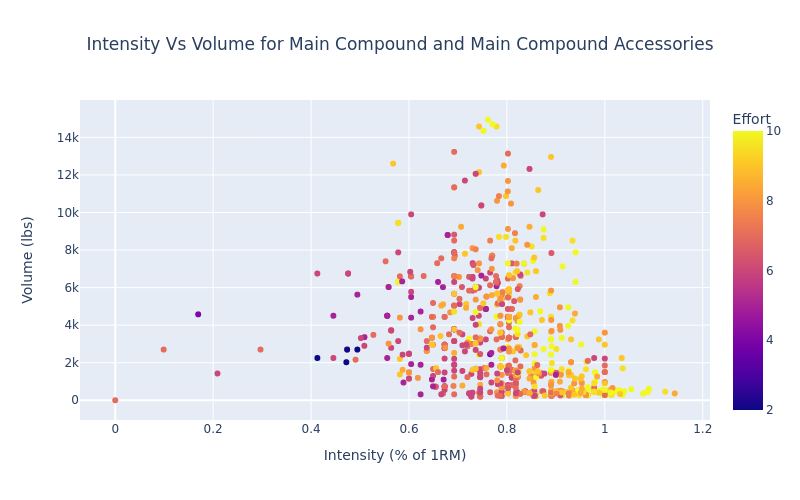
\includegraphics[scale=0.55]{images/ch3/IntensityVsVolume.png}
    \caption{A graph comparing intensity and volume. Note how there is a clear peak in volume between $60\%$-$80\%$.} 
    \label{fig:IntensityVsVolumeGraph}
\end{figure}

The explanation for the peak in volume is rather simple. It is due to the data being collected by a powerlifter, a sport that does not require much in the way of endurance, which skews the data as a result. This skewing of the data will come up again and be discussed more thoroughly in the next section, which is concerned with volume and effort.


\subsection{Property 2: Volume and Effort}
\label{sec:PotentialSurfaceIntuitiveRelationshipsBetweenVariablesVolumeAndEffort}

The next question is what happens when effort increases or decreases across all intensities. As effort increases more sets will be able to be completed, more reps will be able to be completed in each set, or more weight will be able to be lifted. If the increase in effort is large enough, some combination of sets, reps, and weight could all increase. The opposite is true if effort decreases. Again, it should be clear that sets and reps are directly proportional to volume, implying an increase in either one will increase volume. Putting all of this together, as effort increases volume will increase and as effort decreases volume will decrease.

\begin{figure}
    \centering
    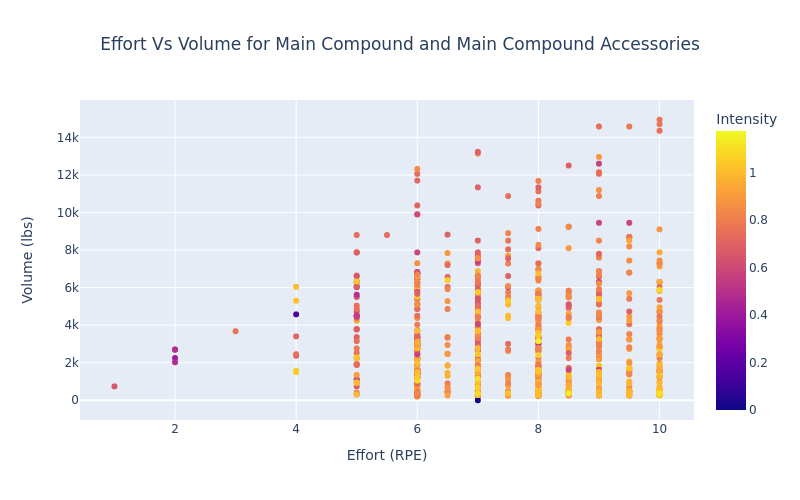
\includegraphics[scale=0.55]{images/ch3/EffortVsVolume.png}
    \caption{A graph comparing effort and volume. Note how there appears to be no correlation between volume and effort.}
    \label{fig:EffortVsVolumeGraph}
\end{figure}
\begin{figure}
    \centering
    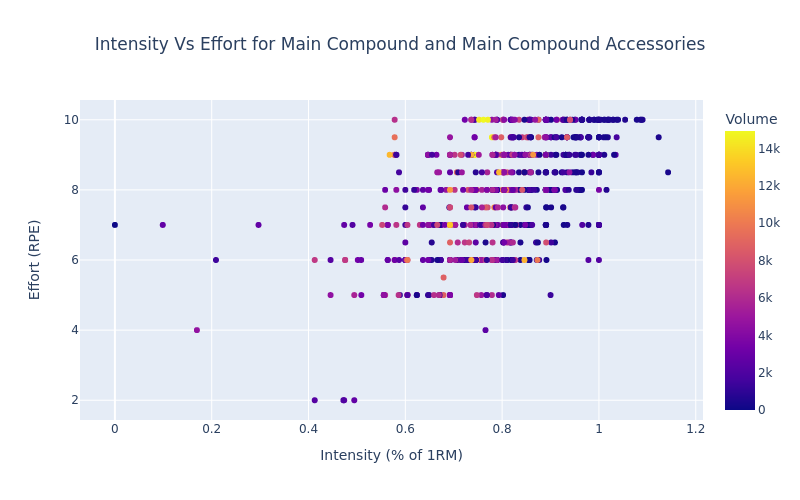
\includegraphics[scale=0.55]{images/ch3/IntensityVsEffort.png}
    \caption{A graph comparing effort and intensity. Note how the intensity tends to increase with higher effort values. This is the result of a powerlifters goal to increase a 1RM.}
    \label{fig:EffortVsIntensity}
\end{figure}

However, in figure \ref{fig:EffortVsVolumeGraph}, which compares volume and effort, volume does not seem to correlate with effort as previously mentioned. Only at the extreme values of each RPE rating does the behavior seem to follow. When looking at the graph as a whole there appears to be no pattern. The reason for this is the same as the previous section. A powerlifter collected the data and the goal of a powerlifter, above all, is to maximize weight. This goal can be seen in figure \ref{fig:EffortVsIntensity}, where intensity positively correlates with effort. What figure \ref{fig:EffortVsIntensity} is saying is that as effort increases the lifter chose to increase weight over sets and reps. Increasing weight, or intensity, will not increase volume as much as if sets and reps were increased due to the previously established fact that volume at higher intensities is necessarily limited by effort. This is a clear bias in the data set, and explains why volume is seemingly constant in figure \ref{fig:EffortVsVolumeGraph}. Given a sport that is more concerned with rep maxes, such as crossfit, the effort vs intensity graph would level out because lower intensities would be pushed for as many reps as possible, creating maximal effort sets with lower intensities. \footnote{This is a perfect example to demonstrate how effort and intensity are two different concepts.} In order to have maximal effort sets with lower intensities either sets, reps, or both sets and reps will need to increase, forcing volume to increase considerably and restoring the correlation between effort and volume previously discussed.


\subsection{Property 3: Volume and Fatigue}
\label{sec:PotentialSurfaceIntuitiveRelationshipsBetweenVariablesVolumeAndFatigue}

Fatigue will necessarily limit volume. The reasoning behind this is simple, the more fatigued you are the less work you can safely do. There can be many sources of fatigue but they will all have the same effect of limiting volume. At the extreme, fatigue will make it so no work can be done at all and hence $0$ volume can be tolerated. This is a state that should be be avoided at all costs, as it is the epitome of over training. When fatigue is at a minimum a lifter will be able to reach there highest potential in there current state. Note that fatigue cannot add to a lifters abilities, it can only diminish them. This is true regardless of effort. No matter how much effort a lifter puts into a set, they would have always been able to lift more weight had they been less fatigued.


\subsection{Property 4: Sets and Reps}
\label{sec:PotentialSurfaceIntuitiveRelationshipsBetweenVariablesSetsAndReps}

With effort, intensity, and fatigues relation to volume being explored, sets and reps are all that's left. It may be tempting to conclude that volume should be constant given a particular weight and effort. This conclusion can be reached by looking at equations \ref{eq:BaseVolumeEquation} and \ref{eq:IntensityBasedVolumeEquation}, where once the weight and effort are known sets and reps would just vary inversely to ensure volume remains constant. Again, while mathematically true, the limits of the human body need to be considered. Evidence that the relationship between sets and reps is not perfectly inverse is shown in figure \ref{fig:SetsVsReps}, where a slight drop in sets from the expected inverse pattern is seen. This favoritism between sets and reps will of course mean volume is no longer constant given a particular intensity and effort, and as such will be known as the \textit{volume skew}.
%This can be attributed to a lack of \textit{endurance}, where sets with a greater number of reps  require more endurance than sets with less reps. Powerlifters are eternally known for having no endurance, so it should come as no surprise that they will favor more sets over reps.

\begin{figure}[h]
    \centering
    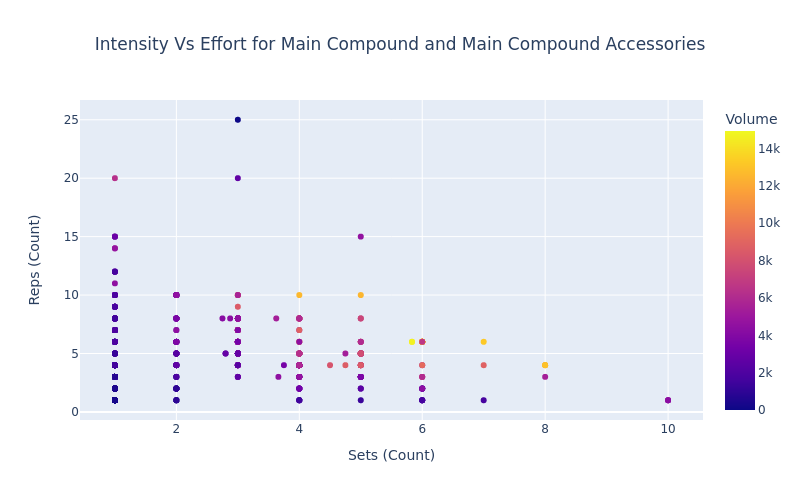
\includegraphics[scale=0.55]{images/ch3/SetsVsReps.png}
    \caption{A graph comparing average reps and sets for main compound and main compound accessory lifts. Note how the relationship is not perfectly inverse. Don't assume any volume skew seen in this graph is necessarily true for all the data, as this plot shows many exercises over a large time span. Finding volume skew will eventually need to be done on a per exercise basis across time.}
    \label{fig:SetsVsReps}
\end{figure}

\subsection{Property 5: Bounded Volume}
\label{sec:PotentialSurfaceIntuitiveRelationshipsBetweenVariablesBoundedVolume}

Unbounded volume occurs when volume continually increases, allowing for the model to ask for an infinite amount of work to be done. This presents a serious issue because this is not possible for a lifter to complete, and is especially problematic considering the purpose of this entire chapter is to establish what is possible and what is not possible. As such, volume will need to be bounded. This could mean that volume reaches a global maximum or, preferably to allow for property 1.b to be true, volume should reach a plateau. Either way, once volume is bounded a maximum achievable volume can be established.

\subsection{Property 6: 1RM Estimations}
\label{sec:PotentialSurfaceIntuitiveRelationshipsBetweenVariables1RMEstimations}

Being able to accurately predict a lifters 1RM is extremely important. There are several reasons knowing a lifters current 1RM is important. First is because of the models dependence on knowing the lifters current 1RM which will be discussed in section \ref{sec:PotentialSurfaceLinearRegressionAndTimeSeriesProblems}. Secondly, it is an important piece of information for tracking progress. The entire goal of a powerlifter is to increase there 1RM over time, which makes it a good measure of progress. Lastly, it is simply just good information for the lifter to know. If the prediction is good enough then it can be used to tell a lifter what weight is safe to load when attempting a new 1RM. This estimation will only be as useful as it is accurate, so, before moving forward an acceptable error needs to be established. If the predicted intensity is, on average, within $1\%$ of the actual intensity then the model will be considered 'accurate', although greater accuracy could not hurt.

By this point it should be obvious the crux of the problem in question will require finding a lifters volume tolerance across intensity and effort, as well as the lifters volume skew between sets and reps. In order to solve this problem, a surface will need to be found that exhibits the appropriate behaviors and then that surface will need to be fitted to the data. These surfaces will be called \textit{potential surfaces}, because they represent a lifters potential performance. It is important to conceptualize that every combination of sets, reps, weight, and effort defined by a potential surface is theoretically possible for a lifter to complete. This is the foundation this entire book will build off of.


\section{Linear Regression and Time Series Problems}
\label{sec:PotentialSurfaceLinearRegressionAndTimeSeriesProblems}

Before moving forward with the goal of finding a surface of best fit using the data set and linear regression, the limits of linear regression need to be considered. Looking at the data set, it should be clear that it is a time series: the data points are collected over time, and data points nearer in time have greater importance than data points farther away in time. Linear regression assumes that all the data points are uncorrelated, which is clearly untrue with time series data. To reconcile the differences between working with linear regression and a time series data set, two things can be done.

The first step that can be taken is to limit the time frame that linear regression is run over. Sets, reps, volume, and the volume skew can all vary through time, but not necessarily in direct linear relation to time. As an example of this, consider seasonal training, which some powerlifters choose to employ. In the off season intensities will drop, volume will increase, and the emphasis on training may shift to hypertrophy over strength. In the on season intensities will increase, volume will necessarily decrease, and the emphasis on training will shift to strength over hypertrophy. This will result in shifts in the number of sets and reps being done over time. To capture these changes over time several techniques can be used. The exact equations that determine what data points are included and to what extent they are considered will be discussed more in chapter \ref{sec:TimeFrame}. That being said, some notation is required to continue. The general notation used to show which data points will be used when performing linear regression is shown in equation \ref{eq:TimeFrame}. The exact length of the time frame, $t_f$, along with any other specifics, will be discussed in chapter \ref{sec:TimeFrame}. Throughout the rest of this book equation \ref{eq:TimeFrame} will be written short hand as $t_i\in \{ T \}$ In an effort to save space.

\begin{equation}
    \label{eq:TimeFrame}
    %t_t\le t_i\le t_t+t_f
    t_i \in\{ t_t, t_t+1,\dots,t_t+t_f \}
    \equiv t_i \in \{ T \}
\end{equation}
\centerline{where}
\begin{equation*}
    \begin{split}
        t_i &\equiv \text{The time component of an arbitrary data point }i \\
        t_t &\equiv \text{An arbitrary target time} \\
        t_f &\equiv \text{The time frame linear regression will be run over} \\
        T & \equiv \text{A shorthand notation representing the set of all allowed times}
    \end{split}
\end{equation*}

The second step that can be taken is to remove weights correlation with time. Weight correlating with time makes intuitive sense, as the goal of a powerlifter is to continually increase weight over time. As an example, say a lifter starts out with a 1RM of $300$ lbs on squat, but through training is able to increase that weight over time to $800$ lbs. It should be obvious from the example that weight has a positive correlation with time. To fix this, weight will be replaced by intensity. This will remove the correlation with time because intensity is calculated using an exercises 1RM, which itself changes with time, canceling out any effects from an increase in weight through time. To show this the previous example will be used again. Despite weight increasing over time, intensity would generally be limited to the range $0\le I\le 1$ because the lifter would set new 1RM's over time, thereby forcing the intensities to be generally less than $1$.

Having an accurate tracking of a lifters 1RM over time becomes an important dependence for the model now that weight is replaced by intensity. For a powerlifter, this is generally not a problem as a lifts 1RM is usually tested once a macrocycle. Problems arise however when things like injuries, or other unplanned problems occur. During these situations a lifters 1RM is not known and can change rapidly or extremely slowly over time. A solution to problems like this will be explored in sections \ref{sec:TimeFrameDynamicTimeFrameAnalysis} and \ref{sec:TimeFrameInjuriesAndChanges}.


\section{The Effort-Fatigue Model}
\label{sec:PotentialSurfaceEffortFatigueModel}

While exploring the intuitive relationships between variables a large amount of emphasis was placed on volume, with most variables being discussed in relation to volume. Despite this, this section is more concerned with how the surface is going to be defined, which will not involve directly involve volume. Instead, the general idea of how the surfaces presented in the next couple sections were conceptualized will be discussed. Within each surfaces chapter, there will be a discussion about how the surface abides by the intuitive behaviors, if at all.

With that, the starting point of every surface is amusingly simple, and can be summed up in the following phrase: Performance is effort diminished by fatigue. To be more specific, performance is equal to total effort diminished by total fatigue. It is tempting to say that, for a powerlifter, performance is simply the weight that is lifted, making $P=w$. However, remembering that these surfaces will eventually be fitted to the data using linear regression and after the discussion in section \ref{sec:PotentialSurfaceLinearRegressionAndTimeSeriesProblems} it should be clear that intensity should be used in the place of weight to measure performance, making $P=I$. Equation \ref{eq:PerformanceProxy} shows an approximate form for the effort-fatigue model.

\begin{equation}
	\label{eq:PerformanceProxy}
	\begin{split}
			P &\hat{=} E_{tot}\hat{-}F_{tot} \\
			I &\hat{=} E_{tot}\hat{-}F_{tot}
	\end{split}
\end{equation}

The $\hat{=}$ symbol in this case means "something like". It is chosen to mean this over something like the $\approx$ symbol because these equations are approximations in the loosest sense. The equations in this section merely form a rough template for later chapters to fully realize. The $\hat{-}$ symbol means "diminished by". The true mathematical interpretation of the $\hat{-}$ symbol is left for future chapters to define.

After performance, total effort is the next easiest term to understand as it directly correlates to how effort was discussed in section \ref{sec:CommonTermsSection}. The only effort that can be applied is by the lifter themselves, no other external factor can 'add effort' to a lifters workout. \footnote{An argument could be made for pre-workout, sugar rushes, a lifter 'getting in there head', or adrenaline dumps 'adding effort', but these are only tools to help a lifter to exert more effort, not tools to generate more effort in and of themselves. Even with these tools, at the end of the day, the effort still has to come from the lifter themselves.} Given this, $E_{tot}$ can be nicely summed up in equation \ref{eq:TotalEffort}. Because there is only one source of effort, a true equality sign can be used. $\epsilon_1$ is a constant that will need to be found after performing linear regression on whatever concrete representation of the surface the next few chapters decide upon.

\begin{equation}
	\label{eq:TotalEffort}
	E_{tot}=\epsilon_1 E
\end{equation}

Total fatigue is more complicated, as there are several different types of fatigue that contribute to it's total. Given the four different types of fatigue listed in section \ref{sec:ModifiedFatigueCategories}, total fatigue can be represented as follows. Total fatigue is more open to intrepretation than total effort, hence the $\hat{=}$ symbol.

\begin{equation*}
	F_{tot} \hat{=} \epsilon_2 F_l+\epsilon_3 F_w+\epsilon_4 F_e+\epsilon_5 F_s
\end{equation*}

Section \ref{sec:AugmentedDataSet} introduced indexes to represent inter-workout and inter-exercise fatigue. These data points can be directly used in the above equation, however as discussed in section \ref{sec:AugmentedDataSet} the index values only represent the fatigue present before the exercise is performed. The fatigue generated from the current exercise needs to be considered to avoid scenarios where the lifter fails a lift due to being too fatigued to make it through the entire exercise. This is where inter-set fatigue matters. Inter-set fatigue will increase in proportion to to total number of reps done. Two additional terms can be added to measure the fatigue generated from sets and reps individually.

\begin{equation*}
	F_{tot} \hat{=} \epsilon_2 F_l+\epsilon_3 F_w+\epsilon_4 F_e+\epsilon_5 sr+\epsilon_6 s+\epsilon_7 r
\end{equation*}

Finally, the approximate form of the effort-fatigue model can be defined, and is shown in equation \ref{eq:PotentialSurfaceEquation}. Again, this may seem like a finished equation, but remember this is just a template. The surfaces in the next several chapters will create final equations to concretely realize the ideas of the effort-fatigue model, apply constraints, and enforce desired behavior. These equations may take very different forms, but the general idea of the effort-fatigue model still stands behind them.

\begin{equation}
	\label{eq:PotentialSurfaceEquation}
	\begin{split}
		I & \hat{=} E_{tot}\hat{-}F_{tot} \\
		I & \hat{=} \epsilon_1 E\hat{-}\left( 
			\epsilon_2 F_l+\epsilon_3 F_w+\epsilon_4 F_e+\epsilon_5 sr+\epsilon_6 s+\epsilon_7 r
		\right)
	\end{split}
\end{equation}

Before going to the next chapters, it is worth mentioning that latent fatigue will be discussed in chapter \ref{sec:}. It has it's rightful place in the potential surface, but it's implications are so broad that they need a chapter of there own. Until chapter \ref{sec:} the effects from latent fatigue will not be considered. For now, think of it as though $\epsilon_2$ were set to $0$. 


\chapter{Surface 1: The Basic Surface}
\label{sec:PotentialSurfaceTheBasicSurface}

The first surface to explore takes the effort-fatigue model in and makes as few changes as possible, treating the $\hat{-}$ symbol to mean literal subtraction and the $\hat{=}$ to mean literal equality. The first change it makes is to center the surface at $(s=1,r=2,I=\epsilon)$ so that the peak in intensity occurs with one set of one rep, matching the lifters 1RM. The second change is adding an error term, represented by $\epsilon$. This is a necessary term to add to perform linear regression. The next, and most substantial change, is to total fatigue. The discussion in section \ref{sec:PotentialSurfaceIntuitiveRelationshipsBetweenVariables} needs to be considered. One of the main takeaways from that section is that volume is limited by effort at high intensities. If the total fatigue template presented by the effort-fatigue model is taken as a literal equation, volume will not have the correct behavior as intensity approaches $100$\%. Namely, there will not be diminishing returns in volume as intensity increases because all the relationships with sets and reps are either linear or a linear combination of both of them. To correct for this, the terms containing sets and reps will be squared, creating diminishing returns to volume with respect to intensity that can be adjusted through the constant in front of each term. \footnote{Yes, there are more flexible ways to do this, but using those ways would make it so linear regression could not be performed due to the multiplicative combinations of constants.} With these changes, the total fatigue equation for the basic surface is shown below. 

\begin{equation*}
	F_{tot} = \epsilon_2 F_l+\epsilon_3 F_w+\epsilon_4 F_e+\epsilon_5 (s-1)^2(r-1)^2+\epsilon_6 (s-1)^2+\epsilon_7 (r-1)^2
\end{equation*}

The final form of the basic surface is shown in equation \ref{eq:BasicSurfaceEquation}. Several constraints are applied to the constants, the reasoning of which will be discussed later in the chapter, but the general idea behind them is to limit the surface to behavior that makes sense for the problem at hand. This equation attempts to fully realize all of the intuitive relationships discussed in section \ref{sec:PotentialSurfaceIntuitiveRelationshipsBetweenVariables}. Which intuitive relationships it fulfills and which it does not will be the topics of sections \ref{sec:PotentialSurfaceAnalysisOfProperty2}-\ref{sec:PotentialSurfaceAnalysisOfProperty4}.

\begin{minipage}{\textwidth}
	\begin{equation}
		\label{eq:BasicSurfaceEquation}
		\begin{split}
			I & =\epsilon+\epsilon_1 E-\left( 
				\epsilon_2 F_l+\epsilon_3 F_w+\epsilon_4 F_e+\epsilon_5 (s-1)^2(r-1)^2+\epsilon_6 (s-1)^2+\epsilon_7 (r-1)^2
			\right)
		\end{split}
	\end{equation}
	\centerline{where}
	\begin{equation*}
	    \begin{split}
	        E & \in \{ 1,1.5,2,2.5, \dots ,10 \} \\
	        \epsilon, \epsilon_1, \epsilon_2, \epsilon_3, \epsilon_4, \epsilon_5,\epsilon_6,\epsilon_7 & > 0 \\
	    \end{split}
	\end{equation*}
\end{minipage}\\

To run linear regression the error equation is needed, which is shown below.

\begin{equation*}
    E_{rr}=\sum_{
            \substack{i=0\\ t_i\in \{ T \}}
        }^n \left(
        I_i
        -\epsilon
        -\epsilon_1 E_i
        +\epsilon_2 F_{l,i}
        +\epsilon_3 F_{w,i}
        +\epsilon_4 F_{e,i}
        +\epsilon_5 (s_i-1)^2(r_i-1)^2
        +\epsilon_6 (s_i-1)^2
        +\epsilon_7 (r_i-1)^2
    \right)^2
\end{equation*}

To minimize the error, the partial derivatives of each unknown constant need to be found and each one set equal to zero. An example with $\epsilon$ is shown below.

\begin{equation*}
    \begin{split}
        \frac{\partial E_{rr}}{\partial \epsilon}=
        \frac{\partial}{\partial \epsilon}\sum_{
                \substack{i=0\\ t_i\in \{ T \}}
            }^n \left(
            I_i
            -\epsilon
            -\epsilon_1 E_i
            +\epsilon_2 F_{l,i}
            +\dots
            %+\epsilon_3 F_{w,i}
            %+\epsilon_4 F_{e,i}
            %+\epsilon_5 (s_i-1)^2(r_i-1)^2
            +\epsilon_6 (s_i-1)^2
            +\epsilon_7 (r_i-1)^2
        \right)^2&=0\\
        -2\sum_{
                \substack{i=0\\ t_i\in \{ T \}}
            }^n \left(
            I_i
            -\epsilon
            -\epsilon_1 E_i
            +\epsilon_2 F_{l,i}
            +\dots
            %+\epsilon_3 F_{w,i}
            %+\epsilon_4 F_{e,i}
            %+\epsilon_5(s_i-1)^2(r_i-1)^2
            +\epsilon_6(s_i-1)^2
            +\epsilon_7(r_i-1)^2
        \right)&=0\\
        \epsilon \sum_{\substack{i=0\\ t_i\in \{ T \}}}^n 1 
        +\epsilon_1 \sum_{\substack{i=0\\ t_i\in \{ T \}}} E_i
        -\epsilon_2 \sum_{\substack{i=0\\ t_i\in \{ T \}}} F_{l,i}
        -\dots
        %-\epsilon_3 \sum_{\substack{i=0\\ t_i\in \{ T \}}} F_{w,i}
        %-\epsilon_4 \sum_{\substack{i=0\\ t_i\in \{ T \}}} F_{e,i}
        %-\epsilon_5 \sum_{\substack{i=0\\ t_i\in \{ T \}}}^n (s_i-1)^2(r_i-1)^2
        -\epsilon_6 \sum_{\substack{i=0\\ t_i\in \{ T \}}}^n (s_i-1)^2
        -\epsilon_7 \sum_{\substack{i=0\\ t_i\in \{ T \}}}^n (r_i-1)^2
        &=
        \sum_{\substack{i=0\\ t_i\in \{ T \}}}^n I_i\\
    \end{split}
\end{equation*}

After a similar process is carried out for each unknown constant, equation \ref{eq:LinearRegMatrixEquation} can be used, and the unknown constants can be solved for.

\begin{equation}
    \label{eq:LinearRegMatrixEquation}
	\left[
    \begin{matrix}
        \sum_{i=0}^n 1 &
        \dots &
        -\sum_{\substack{i=0\\ t_i\in \{ T \}}}^n (r_i-1)^2 \\

        \sum_{\substack{i=0\\ t_i\in \{ T \}}}^n  E_i &
        \dots &
        -\sum_{\substack{i=0\\ t_i\in \{ T \}}}^n E_i (r_i-1)^2\\

        \vdots &
        \ddots &
        \vdots \\
        
        \sum_{\substack{i=0\\ t_i\in \{ T \}}}^n (r_i-1)^2 &
        \dots &
        -\sum_{\substack{i=0\\ t_i\in \{ T \}}}^n (r_i-1)^4
    \end{matrix}
    \right]
	\left[
    \begin{matrix}
        \epsilon \\ \epsilon_1 \\ \vdots \\ \epsilon_7
    \end{matrix}
    \right]
    =
	\left[
    \begin{matrix}
        \sum_{\substack{i=0\\ t_i\in \{ T \}}}^n I_i \\
        \sum_{\substack{i=0\\ t_i\in \{ T \}}}^n I_i E_i \\
        \vdots \\
        \sum_{\substack{i=0\\ t_i\in \{ T \}}}^n I_i(r_i-1)^2 
    \end{matrix}
    \right]
\end{equation}

With equations \ref{eq:BasicSurfaceEquation} and \ref{eq:LinearRegMatrixEquation}, this surface is fully defined. After fitting the surface to the data discussed in chapter \ref{sec:DataSection}, graphs similar to the ones shown in figure \ref{fig:SquatPotentialSurfaceAcrossEffort} can be created. Many of the relationships discussed in section \ref{sec:PotentialSurfaceIntuitiveRelationshipsBetweenVariables} are concerned with volume. To give some intuition for volume before moving on, equation \ref{eq:IntensitySubedInVolume} is the result of solving the potential surface for $I$ and substituting it in equation \ref{eq:IntensityBasedVolumeEquation}. The graphs shown in figure \ref{fig:SquatPotentialSurfaceVolumeAcrossEffort} show the volume surface generated from this potential surface.

\begin{equation}
    \label{eq:IntensitySubedInVolume}
    \begin{split}
    		v = & srI l_{1RM} \\
    			= & l_{1RM} sr \left( 
    			\epsilon+
    			\epsilon_1 E-
    			\epsilon_2 F_l-
    			\epsilon_3 F_w-
    			\epsilon_4 F_e-
    			\epsilon_5(s-1)^2(r-1)^2-
    			\epsilon_6(s-1)^2-
    			\epsilon_7(r-1)^2
    		\right)
    \end{split}
\end{equation}

\begin{figure}[htbp]
    \centering
    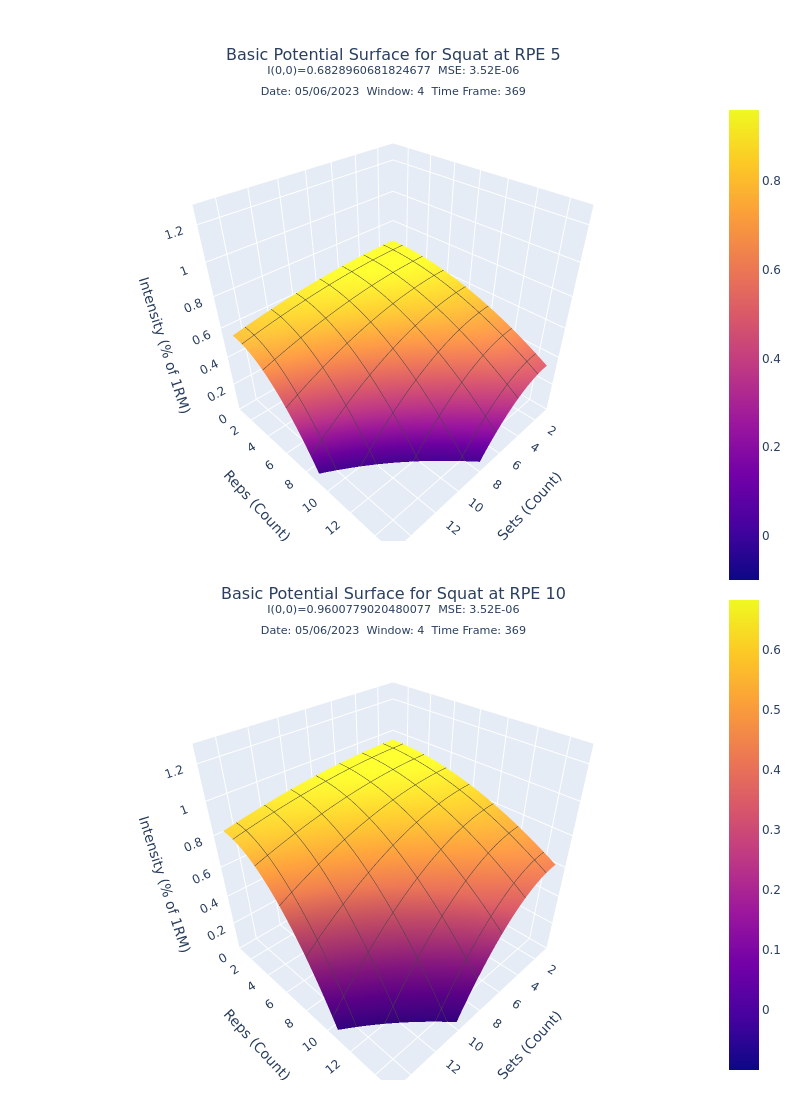
\includegraphics[scale=0.55]{images/ch3/PotentialSurface/DualSquat.Effort[5,10].basic.png}
    \caption{The potential surface fitted to squat data at various effort levels. The window and time frame values will be discussed in chapter \ref{sec:TimeFrame}. For now, the $I(1,1)$ and MSE values are the most important.}
    \label{fig:SquatPotentialSurfaceAcrossEffort}
\end{figure}

\begin{figure}[htbp]
    \centering
    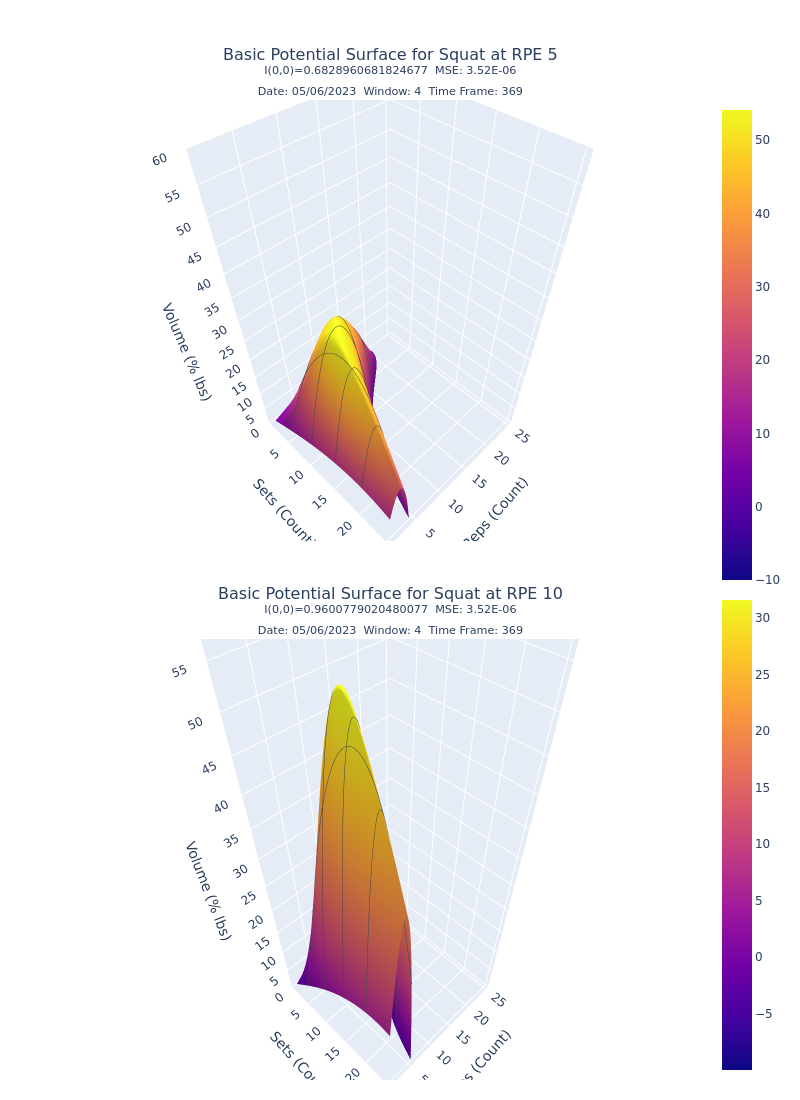
\includegraphics[scale=0.55]{images/ch3/Volume/DualSquat.Effort[5,10].basic.png}
    \caption{The volume surface resulting from the potential surface fitted to squat data at various effort levels.}
    \label{fig:SquatPotentialSurfaceVolumeAcrossEffort}
\end{figure}

\section{Analysis of Property 1.a: Volume and Intensity}
\label{sec:PotentialSurfaceAnalysisOfProperty1a}

Property 1.a states that volume should approach the lifters 1RM as intensity increases. To prove this two things need to happen. It needs to be proven that equation \ref{eq:BasicSurfaceEquation} has a single global maximum and no minimum. This maximum should equal the lifters current 1RM. Given that this is the case, it then needs to be proven that equation \ref{eq:IntensitySubedInVolume} has a  minimum at the same point that equation \ref{eq:BaseIntensityEquation} has it's maximum. This minimum also needs to equal the value of equation \ref{eq:BaseIntensityEquation} at its maximum. Given that all of that is true, it can be said that the basic surface exhibits property 1.a because volume has a minimum at the same location intensity has a global maximum, meaning intensity increases from all directions to that point where volume has a value equal to the lifters current 1RM.

To begin, the maximum of equation \ref{eq:BaseIntensityEquation} needs to be found. This will require the gradient of that function, shown below.

\begin{equation*}
	\nabla I =
	\left[
	\begin{matrix}
		\frac{\partial I}{\partial E} \\
		\frac{\partial I}{\partial F_l} \\
		\frac{\partial I}{\partial F_w} \\
		\frac{\partial I}{\partial F_e} \\ 
		\frac{\partial I}{\partial s} \\
		\frac{\partial I}{\partial r} \\
	\end{matrix}
	\right] =
	\left[
	\begin{matrix}
		\epsilon_1 \\
		-\epsilon_2 \\
		-\epsilon_3 \\
		-\epsilon_4 \\
		-2(s-1)\left( \epsilon_5(r-1)^2+\epsilon_6 \right) \\
		-2(r-1)\left( \epsilon_5(s-1)^2+\epsilon_7 \right) \\
	\end{matrix}
	\right]
\end{equation*}

To find critical points where a maximum could occur the gradient will be set to zero, $\nabla I=0$, and all the variables can be solved for. Looking at the above equation, there are only two variables remaining, $s$ and $r$. This means that all the variables $E$,$F_l$,$F_w$, and $F_e$ can be any value and the location of the maximum will remain unchanged. Given that only the last two equations of $\nabla I$ effect the result, the problem of finding critical points is essentially rendered down to a two dimensional problem. After some algebraic manipulation, it can be shown that the only critical point is $(s=1,r=1)$.

Now, given the critical point at $(s=1,r=1)$ it needs to be proven to be a maximum. The simplification to a two dimensional problem will be used here, and the standard determinant equation can be used to determine concavity.

\begin{equation*}
	\begin{split}
		\partial_{ss}I & = -2\left( 
			\epsilon_5(r-1)^2+\epsilon_6 
		\right) \\
		\partial_{rr}I & = -2\left( 
			\epsilon_5(s-1)^2+\epsilon_7 
		\right) \\
		\partial_{sr}I & = -4 \epsilon_5 (s-1)(r-1) \\
		D(s=1,r=1) & = \partial_{ss}I(1,1) \partial_{rr}I(1,1)-\left(
			\partial_{sr} I(1,1)
		\right)^2 = 4\epsilon_6 \epsilon_7
	\end{split}
\end{equation*}

Given the constraints on equation \ref{eq:BaseIntensityEquation} it can be said that $D(s=1,r=1)>0$. Given this and the fact that $\partial_{ss}I(s=1,r=1)=-2\epsilon_6$, which is $<0$, it can be stated that the critical point $(s=1,r=1)$ is a maximum. This maximum needs to be shown to equal the lifters 1RM. To obtain this, equation \ref{eq:BaseIntensityEquation} is simply evaluated at $(s=1,r=1)$ and scaled by $l_{1RM}$ to get weight instead of intensity. The result is shown in equation \ref{eq:BasicSurface1RMPred}, which represents what the model thinks the lifters 1RM is. This is an important concept, especially because of the discussion in section \ref{sec:PotentialSurfaceLinearRegressionAndTimeSeriesProblems}, and will be returned to in section \ref{sec:PotentialSurface1RMEstimations}.

\begin{equation}
	\label{eq:BasicSurface1RMPred}
	l_{1RM} I(s=1,r=1)=l_{1RM} \left(
		\epsilon+
    		\epsilon_1 E-
    		\epsilon_2 F_l-
    		\epsilon_3 F_w-
    		\epsilon_4 F_e
    	\right)
\end{equation}

With that, the first part of the proof is complete. The intensity equation has a single max that represents the lifters current 1RM. The second part of the proof relies on finding a minimum of the volume surface. To do this, the gradient of equation \ref{eq:IntensitySubedInVolume} is needed.

\begin{equation*}
	\begin{split}
		\nabla v = & \left[\begin{matrix}
			\frac{\partial v}{\partial E} \\
			\frac{\partial v}{\partial F_l} \\
			\frac{\partial v}{\partial F_w} \\
			\frac{\partial v}{\partial F_e} \\
			\frac{\partial v}{\partial s} \\
			\frac{\partial v}{\partial r} \\
		\end{matrix}\right]=
		\left[\begin{matrix}
			l_{1RM} \epsilon_1 sr \\
			-l_{1RM} \epsilon_2 sr \\
			-l_{1RM} \epsilon_3 sr \\
			-l_{1RM} \epsilon_4 sr \\
			\partial_s v \\
			\partial_r v\\
		\end{matrix}\right] \\
		\partial_s v = & l_{1RM} \left(
			\epsilon r+
			\epsilon_1 Er-
			\epsilon_2 F_l r-
			\epsilon_3 F_w r-
			\epsilon_4 F_e r-
			\epsilon_7 r(r-1)^2	-
			\left( 
				\epsilon_5 r(r-1)^2+\epsilon_6 r
			\right)	
			(3s^2-4s+1)
		\right) \\
		\partial_r v = & l_{1RM} \left(
			\epsilon s+
			\epsilon_1 Es-
			\epsilon_2 F_l s-
			\epsilon_3 F_w s-
			\epsilon_4 F_e s-
			\epsilon_6 s(s-1)^2	-
			\left( 
				\epsilon_5 r(r-1)^2+\epsilon_7 s
			\right)	
			(3r^2-4r+1)
		\right) \\
	\end{split}
\end{equation*}

This time the gradient does not remove any variables, making the simplification that was previously performed unusable. However, looking at the first four equations of the gradient in context of the last two it is clear that the only critical point occurs at $(s=0,r=0)$. However, looking at figures \ref{fig:SquatPotentialSurfaceVolumeAcrossEffort} there appears to be another critical point that represents a maximum. The reason for that is because those graphs have constant values for $E$, $F_l$, $F_w$, and $F_e$. This removes the first four equations of the gradient and as such makes room for another critical point. Given the terms with the $E$, $F_l$, $F_w$, and $F_e$ variables are linear it should come as no surprise that those variables prevent a maximum from occurring, allowing infinite growth in relation to any of the variables.

Going back to the critical point, it needs to be be proven that it is a minimum. However, without the previous simplification the determinant of the Jacobian matrix would be needed to specify if this critical point is a minimum or maximum. Solving that analytically is near impossible, so it will have to suffice looking at the graphs of figure \ref{fig:SquatPotentialSurfaceVolumeAcrossEffort} for proof that this critical point is a minimum. 

Now, this critical point does not match the critical point found from the intensity equation. This presents a problem because unless the points are the same the whole proof falls apart. The saving nuance comes from the domain of the problem, with both $s$ and $r$ being restricted to being $\ge 1$ in section \ref{sec:UnitsOfMeasurement}. This restriction means the minimum in relation to this problem is $(s=1,r=1)$, matching the maximum of equation \ref{eq:BasicSurfaceEquation}. Given this, all that is left to prove is that volume at this critical point is equal to the lifters current 1RM found previously, which is shown in the equation below. With that, it is proven that this surface properly exhibits property 1.a.

\begin{equation}
	v(s=1,r=1)=l_{1RM} \left(
    			\epsilon+
    			\epsilon_1 E-
    			\epsilon_2 F_l-
    			\epsilon_3 F_w-
    			\epsilon_4 F_e 
    	\right) = I(s=1,r=1)
\end{equation}

\section{Analysis of Property 2: Volume and Effort}
\label{sec:PotentialSurfaceAnalysisOfProperty2}

It needs to be shown that volume increases with increased effort and decreases with decreased effort. As such, the changes in $v$ relating to changes in $E$ are desired, requiring the partial derivative of equation \ref{eq:IntensitySubedInVolume} with respect to $E$.

\begin{equation*}
    \begin{split}
    		\frac{\partial v}{\partial E} & =
    		\frac{\partial}{\partial E} l_{1RM}sr\left( 
    			\epsilon+
    			\epsilon_1 E-
    			\epsilon_2 F_l-
    			\epsilon_3 F_w-
    			\epsilon_4 F_e-
    			\epsilon_5(s-1)^2(r-1)^2-
    			\epsilon_6(s-1)^2-
    			\epsilon_7(r-1)^2
    		\right) \\
    		& =\epsilon_1 l_{1RM} sr
    \end{split}
\end{equation*}

If $\partial_{E}v$ is always $>0$, then it can be said the function is strictly increasing, meaning volume strictly increases with increased effort. The following inequalities are given in section \ref{sec:UnitsOfMeasurement}.

\begin{equation*}
    \begin{split}
        s \ge & 1 \\
        r \in & \{ \mathbb{R}\ge 1 \} \\
        w > & 0
    \end{split}
\end{equation*}

Given that $l_{1RM}$ is a weight, the following conclusion can be made from the above inequalities.

\begin{equation*}
    \epsilon_1 l_{1RM} sr> 0 \textbf{ iff } \epsilon_1> 0
\end{equation*}

Therefore, it can be concluded that volume increases with increased effort if and only if $\epsilon_1> 0$. A similar argument can be made that proves volume decreases with decreased effort if and only if $\epsilon_1> 0$. Of course, this behavior will need to be ensured, so a constraint is be placed on $\epsilon_1$. This constraint is listed in equation \ref{eq:PotentialSurfaceEquation}.

\section{Analysis of Property 3: Volume and Fatigue}
\label{sec:PotentialSurfaceAnalysisOfProperty3}

For property 2, it needs to be shown that volume decreases with increased fatigue. Similar to the previous section, partial derivatives are required. A partial derivative is needed for every fatigue term. Luckily all the fatigue terms are similar in nature, so for brevity only one will be analyzed here and it should be known that the other fatigue terms will follow the same behaviors. To begin, the partial derivative of equation \ref{eq:IntensitySubedInVolume} with respect to $F_l$ is required.

\begin{equation*}
    \begin{split}
    		\frac{\partial v}{\partial F_l} & =
    		\frac{\partial}{\partial F_l} l_{1RM} sr\left( 
    			\epsilon+
    			\epsilon_1 E-
    			\epsilon_2 F_l-
    			\epsilon_3 F_w-
    			\epsilon_4 F_e-
    			\epsilon_5(s-1)^2(r-1)^2-
    			\epsilon_6(s-1)^2-
    			\epsilon_7(r-1)^2
    		\right) \\
    		& = -\epsilon_2 l_{1RM} sr
    \end{split}
\end{equation*}

This time, if $\partial_{F_l}v$ is always $<0$ then it can be said the function is strictly decreasing and volume decreases with increased fatigue. The same inequalities that were presented in previous section can be used here and the following statement can be made.

\begin{equation*}
    -\epsilon_2 l_{1RM} sr< 0 \textbf{ iff } \epsilon_2> 0
\end{equation*}

This proves that volume decreases with fatigue if and only if $\epsilon_2>0$. Just like the previous section, a similar argument can be made to prove that volume increases with decreased fatigue. This constraint will need to be applied to $\epsilon_2$, $\epsilon_3$, $\epsilon_4$, $\epsilon_5$, and $\epsilon_7$ as they are all part of $F_{tot}$. These constraints are listed in equation \ref{eq:PotentialSurfaceEquation}. The next section should offer a break from the monotony of this section.

\section{Analysis of Property 4: Sets and Reps}
\label{sec:PotentialSurfaceAnalysisOfProperty4}

Property 4 is concerned with how sets and reps change, mainly with regard to volume skew. As such, it needs to be shown that the model is capable of determining volume skew. An initial look at the potential surface can't hurt. Looking at the potential surface equation the only place where differences between $s$ and $r$ can arise are with the $\epsilon_6$ and $\epsilon_7$ terms, so it makes sense to reason that ratio of those constants will somehow measure volume skew. Exactly how they measure volume skew will need to be determined by calculating the volume underneath the volume surface on either side of the plane $s=r$. Once that is done, the ratio of total volume skewing towards sets and reps respectively can be calculated. 

To measure the total volume on either side of the plane $s=r$ several double integrals will need to be calculated. Given the non-concave nature of the volume surface, calculating the total volume on either side of the $s=r$ plane will require the volume surface to be broken up into $4$ regions. These regions are:

\begin{itemize}
	\item $1\le r\le s$ and $0\le s \le S_d$ where $S_d$ is the point where the volume surface intersects the line $s=r$ on the $sr$ plane.
	\item $1\le s\le r$ and $0\le r \le R_d$ where $R_d$ is the point where the volume surface intersects the line $s=r$ on the $sr$ plane.
	\item $1\le r\le S_t$ and $S_d \le s\le S_e$ where $S_t$ is the intersection of the volume surface on the $sr$ plane solved for $s$ and $S_e$ is the the point where the volume surface intersects the $s=1$ line on the $sr$ plane.
	\item $1\le s\le R_t$ and $R_d \le r\le R_e$ where $R_t$ is the intersection of the volume surface on the $sr$ plane solved for $r$ and $R_e$ is the the point where the volume surface intersects the $r=1$ line on the $sr$ plane.
\end{itemize}

Note that due to the nature of the line $s=r$, $S_d=R_d$. In integral form, the equation will take the form shown in equation \ref{eq:BasicSurfaceVolumeSkew}. Note that this equation creates a fraction of sets over reps. The inverse of equation \ref{eq:BasicSurfaceVolumeSkew} would represent reps over sets. Either way would work as long as it is known which form is used, so, to be clear, the form of sets over reps will be used for the rest of this section.

\begin{minipage}{\textwidth}
	\begin{equation}
	   \label{eq:BasicSurfaceVolumeSkew}
	   v_s=\frac{
	   	\int_{1}^{S_d}\int_{1}^{s}v\;drds+
	   	\int_{S_d}^{S_e}\int_{1}^{R_t}v\;drds
	   }{
	   	\int_{1}^{R_d}\int_{1}^{r}v\;dsdr+
	   	\int_{R_d}^{R_e}\int_{1}^{S_t}v\;dsdr
	   }
	\end{equation}
	\centerline{where}
	\begin{equation*}
		\begin{split}
			v & \equiv \text{ equation \ref{eq:IntensitySubedInVolume}} \\
			S_d=R_d & =\left(
				\frac{
	   				-\epsilon_6-\epsilon_7+\sqrt{
	   					(\epsilon_6+\epsilon_7)^2+
	   					4\epsilon_5(
	   						\epsilon+
	   						\epsilon_1E-
	   						\epsilon_2F_l-
	   						\epsilon_3F_w-
	   						\epsilon_4F_e
	   					)
	   				}
	   			}{
	   				2\epsilon_5
			   	}\right)^{\frac{1}{2}} +1 \\
			S_e & =\left(
				\frac{
					\epsilon+
					\epsilon_1E-
					\epsilon_2F_l-
					\epsilon_3F_w-
					\epsilon_4F_e
				}{
					\epsilon_6
				}
			\right)^{\frac{1}{2}}+1 \\
			R_e & =\left(
				\frac{
					\epsilon+
					\epsilon_1E-
					\epsilon_2F_l-
					\epsilon_3F_w-
					\epsilon_4F_e
				}{
					\epsilon_7
				}
			\right)^{\frac{1}{2}}+1 \\
			S_t & =\left(
				\frac{
					\epsilon+
					\epsilon_1E-
					\epsilon_2F_l-
					\epsilon_3F_w-
					\epsilon_4F_e-
					\epsilon_7(r-1)^2		
				}{
					\epsilon_5(r-1)^2+
					\epsilon_6
				}
			\right)^{\frac{1}{2}}+1 \\
			R_t & =\left(
				\frac{
					\epsilon+
					\epsilon_1E-
					\epsilon_2F_l-
					\epsilon_3F_w-
					\epsilon_4F_e-
					\epsilon_6(s-1)^2		
				}{
					\epsilon_5(s-1)^2+
					\epsilon_7
				}
			\right)^{\frac{1}{2}}+1 \\
		\end{split}
	\end{equation*}
\end{minipage}

Given this equation, the following statements can be made:

\begin{enumerate}
    \item If $v_s<1$ then the total volume from reps is greater than the total volume from sets, which implies that the lifter favors reps for the given exercise, or has a volume skew towards reps for the given exercise.
    \item If $v_s>1$ then the total volume from sets is greater than the total volume from reps, which implies that the lifter favors sets for the given exercise, or has a volume skew towards sets for the given exercise.
    \item If $v_s=1$, then the lifter has no volume skew.
    \item If $\epsilon_6=0$ or $\epsilon_7=0$ then a lifter has the maximum possible skew towards sets or reps respectively. \footnote{This idea will be explored more from volumes perspective in section \ref{sec:PotentialSurfaceUnboundedVolume}.}
\end{enumerate}

Several things are of immediate interest from equation \ref{eq:BasicSurfaceVolumeSkew}. The first is whether or not the top and bottom of the fraction are equivalent. If they are equivalent then this means the surface cannot measure volume skew. Luckily they are not equivalent due to the small differences in the placement of the $\epsilon_6$ and $\epsilon_7$ terms in the integral bounds. The first term on the top and bottom of the fraction may look equivalent because the bounds of integration are the same for both terms, but the order of the variables being integrated prevents this, this time because of the difference between the $\epsilon_6$ and $\epsilon_7$ terms in the volume equation. With this, property 4 is proven to be satisfied as the surface can measure volume skew.

The second thing of interest is that this equation is utterly unusable algebraically. It would be quite nice to see the fraction reduce down to some jumble of constants that would be somewhat palatable, but the second term on the top and bottom of the fraction makes this impossible. The first term on the top and bottom of the fraction would be very tedious to compute by hand, but would technically be possible due to the simplicity of the inner integrals bounds. However, in the second term the $R_t$ and $S_t$ equations present a rather nasty upper bound on the inner integral that would have to be integrated after substituting it in the integral of the volume equation. This just results in more of a mess than it is worth trying to untangle. Because of this, an alternate way to measure volume skew would be helpful to have.

The starting point for creating an approximation for volume skew is noticing that, generally, $S_e$ and $R_e$ each increase with the total volume on there respective sides of the $s=r$ plane. As such, the approximation for volume skew can be represented as the ratio of those terms, shown in equation \ref{eq:BasicSurfaceApproxVolumeSkew}. In order to match equation \ref{eq:BasicSurfaceVolumeSkew}, this equation will also create a fraction of sets over reps.

\begin{equation}
	\label{eq:BasicSurfaceApproxVolumeSkew}
	\begin{split}
		v_s \approx \frac{S_e}{R_e} & =\frac{
			\left(
				\frac{
					\epsilon+
					\epsilon_1E-
					\epsilon_2F_l-
					\epsilon_3F_w-
					\epsilon_4F_e
				}{
					\epsilon_6
				}
			\right)^{\frac{1}{2}}+1
		}{
			\left(
				\frac{
					\epsilon+
					\epsilon_1E-
					\epsilon_2F_l-
					\epsilon_3F_w-
					\epsilon_4F_e
				}{
					\epsilon_7
				}
			\right)^{\frac{1}{2}}+1
		} \\
		& = \frac{
			\epsilon_7^{\frac{1}{2}} \left(
				\left(
					\epsilon+
					\epsilon_1E-
					\epsilon_2F_l-
					\epsilon_3F_w-
					\epsilon_4F_e
				\right)^{\frac{1}{2}}+
				\epsilon_6^{\frac{1}{2}}
			\right)		
		}{
			\epsilon_6^{\frac{1}{2}} \left(
				\left(
					\epsilon+
					\epsilon_1E-
					\epsilon_2F_l-
					\epsilon_3F_w-
					\epsilon_4F_e
				\right)^{\frac{1}{2}}+
				\epsilon_7^{\frac{1}{2}}
			\right)		
		}
	\end{split}
\end{equation}

Because equation \ref{eq:BaseVolumeEquation} cannot be algebraically manipulated, the efficacy of this approximation will need to be shown analytically. The graphs in figure \ref{fig:ApproximateVsActualVolumeSkew} show the true volume skew compared to the approximation for varying values of different $\epsilon$ constants. As the graphs show, the approximation holds well enough to be considered a valid approximation. Of note is that when the actual volume skew equals $1$ so does the approximation. This is important because this is a critical point where the direction of the skew changes, so exactly matching this value in the approximation is important. Also of note is that as the approximation strays from $1$ it gets worse, with large $\epsilon_7$ values being particularly troublesome. The reason $\epsilon_7$ values have a greater error relates to the nature of the fraction. Having a skew towards reps constrains volume skew to be between $0\le v_s<1$ whereas a skew towards sets constrains the fraction to be between $1<v_s\le \infty$. Both scenarios need to represent the same range of values, but the skew towards reps has a much smaller range to do so, which also leaves much less space for error. This weakness of the volume skew approximation can also be seen in graph \ref{fig:ApproximateVsActualVolumeSkewOverTime} where volume skew values $>1$ have much greater separation from there approximated values.

\begin{figure}[htb]
    \centering
    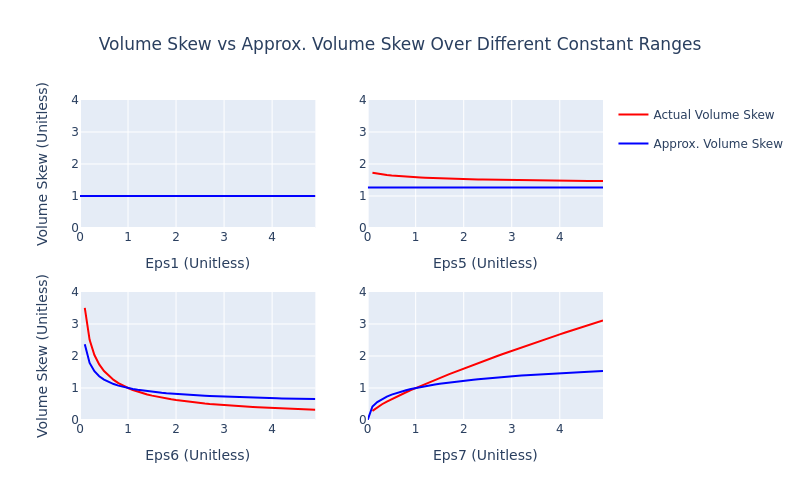
\includegraphics[scale=0.55]{images/ch3/ApproxVsActualVolumeSkew.basic.png}
    \caption{Graphs comparing the approximate and actual volume skew over varrying $\epsilon$ values. Note how the approximation follows the same direction of rate of change of the true volume skew, making it a reasonable approximation for this particular use case.}
    \label{fig:ApproximateVsActualVolumeSkew}
\end{figure}
\begin{figure}[htb]
    \centering
    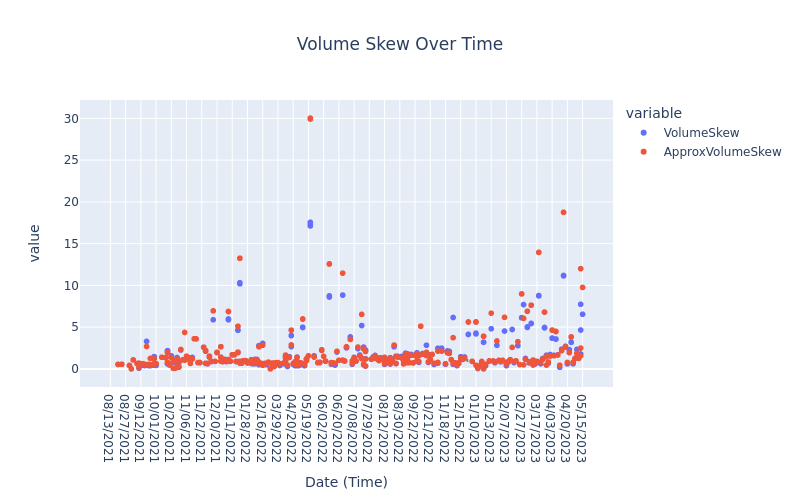
\includegraphics[scale=0.55]{images/ch3/volumeSkewOverTime.png}
    \caption{Graphs comparing the approximate and actual volume skew over time. Note how the volume skew values $>1$ have much greater error.}
    \label{fig:ApproximateVsActualVolumeSkewOverTime}
\end{figure}

Before moving on, there has been so much attention on $\epsilon_6$ and $\epsilon_7$ that $\epsilon_5$ has not been discussed, despite having $s$ and $r$ terms associated with it. The constant $\epsilon_5$ represents the volume that should be possible no matter the magnitude of the volume skew. For example, if $\epsilon_6=0$ and $\epsilon_7>0$ for a given exercise, then the following can be stated about the lifter and the way they perform that particular exercise:

\begin{itemize}
    \item The lifter has a volume skew towards reps.
    \item As the lifter leaves there normal volume skew, they should still be able to perform volume in proportion to $\epsilon_5$ even when $r\to 1$ and the contributions from $\epsilon_7$ diminish.
    \item The volume from $\epsilon_5$ is less than any volume that would have been present if $\epsilon_6>0$ because the relation between $\epsilon_5$ and $\epsilon_6$ is additive.
\end{itemize}

Having this representation for baseline work capacity in the opposing volume skew is important. If it was not present the model would assume when a lifter has a certain volume skew, any volume from the opposing skew would simply not be possible. In reality, this is not the case, some baseline level of volume will always be possible, even in the opposite skew. Do not confuse this with volume tolerance, which represents a maximal volume that a lifter can tolerate rather than a baseline of volume possible in the opposing volume skew.

\section{Analysis of Property 5: (Un)Bounded Volume}
\label{sec:PotentialSurfaceUnboundedVolume}

One way to prove volume is bounded, and hence prove the surface properly exhibits property 5, is to prove that it has a maximum value. Given the discussion in section \ref{sec:PotentialSurfaceAnalysisOfProperty1a} this maximum does appear to be present when $E$, $F_l$, $F_w$, and $F_e$ are all considered to be constant. The question now is if that maximum is always present. Figuring that out will require finding the solution to the $\partial_sv$ and $\partial_rv$ system of equations shown in the gradient of $v$ in section \ref{sec:PotentialSurfaceAnalysisOfProperty1a}. However, analytically solving that system of equations is impossible. To get around this, the problem will be looked at from the perspectives of $\partial_sv$ and $\partial_rv$ individually. As such, the first and second partial derivatives of $v$ with respect to $s$ are shown below. It will be discussed later what changes when the partial derivative with respect to $r$ is chosen instead.

\begin{equation*}
    \partial_s v = l_{1RM} \left(
			\epsilon r+
			\epsilon_1 Er-
			\epsilon_2 F_l r-
			\epsilon_3 F_w r-
			\epsilon_4 F_e r-
			\epsilon_7 r(r-1)^2	-
			\left( 
				\epsilon_5 r(r-1)^2+\epsilon_6 r
			\right)
			(3s^2-4s+1)
		\right)
\end{equation*}
\begin{equation*}
    \partial_{ss}v=-l_{1RM} r
    		\left( 
			\epsilon_5 (r-1)^2+\epsilon_6
		\right)
		(6s-4)
\end{equation*}

A global maximum occurs when $\partial_{ss} v<0$. In order for this to be the case either none of the parenthetical groupings needs to be negative or an even number of the above parenthetical groupings need to be negative. Thr first parenthetical grouping is guarintted to be positive due to the constraints placed on $r$ in section \ref{sec:UnitsOfMeasurement}. The last parenthetical grouping will be $>0$ if $s>\frac{2}{3}$, which is again guaranteed to be true because of the constraints placed on $s$ in section \ref{sec:UnitsOfMeasurement}. This guarantees two of the three parenthetical groupings to be positive, which forces the middle parenthetical grouping to be positive for $\partial_{ss} v$ to be $<0$. The sign of $\epsilon_5$ changes the set of inequalities that define when the middle parenthetical group is $>0$, and hence when a maximum can occur. Table \ref{tab:BoundedVolumeRanges} shows the inequalities and ranges when volume is bounded for various values of $\epsilon_5$ and $\epsilon_6$.

Care has to be taken when $\epsilon_5=0$ or $\epsilon_6=0$, as the behavior of the inequalities is not fully captured by substituting $0$ for $\epsilon_5$ or $\epsilon_6$. A traditional limit cannot be used because inequalities are one sided, and a limit expects a continuous function. Instead, the four scenarios where $\epsilon_5=0$ and $\epsilon_6=0$ will be treated as one sided limits which will be approached from the side where the behavior is already known. By doing this, the sign can be inferred and the one sided nature of the problem. \footnote{The notation used in table \ref{tab:BoundedVolumeRanges} is as follows: given a number $x$, $x^-$ is a smaller number approaching $x$, and $x^+$ is a larger number approaching $x$. This allows for one sided analysis to be completed.} The scenarios where the root is imaginary are also troublesome. However, the same one sided analysis can be extended and used again. Table \ref{tab:BoundedVolumeRanges} shows how the one sided limit works as well as how the ranges over which volume is bounded respond.\footnote{For the purposes of this discussion the constraints placed on $\epsilon_2$-$\epsilon_7$ will be ignored. These constraints will be reconsidered at the end of the discussion.}

\begin{table}[h]
    \centering
    \begin{tabular}{|p{1cm}|p{6cm}|c|}
    		\hline
        Values & Inequalities & Range Where Volume is Bounded \\
        \hline

        $\epsilon_5>0$
        \newline
        $\epsilon_6<0$
        &
        $r> \left(-\frac{\epsilon_6}{\epsilon_5}\right)^\frac{1}{2}+1$
        \newline
        $r< -\left(-\frac{\epsilon_6}{\epsilon_5}\right)^\frac{1}{2}+1$
        &
        $\left( r>\left| \frac{\epsilon_6}{\epsilon_5} \right|^\frac{1}{2}+1 \right) \cup \left( r< -\left| \frac{\epsilon_6}{\epsilon_5} \right|^\frac{1}{2}+1 \right)$
        \\
        \hline
        
        $\epsilon_5>0$
        \newline
        $\epsilon_6=0$
        &
        $r> \left(-\frac{0^-}{\epsilon_5}\right)^\frac{1}{2}+1$
        \newline
        $r< -\left(-\frac{0^-}{\epsilon_5}\right)^\frac{1}{2}+1$
        &
        $\left( r> 1^+ \right) \cup \left( r<1^- \right)$, a.k.a. $r\ne 1$
        \\
        \hline
        
        $\epsilon_5>0$
        \newline
        $\epsilon_6>0$
        &
        $r> (0+\beta i)+1$
        \newline
        $r< (-0-\beta i)+1$
        &
        $(r>1)\cup (r<1)$ a.k.a. All $r$
        \\
        \hline
        
        $\epsilon_5=0$
        \newline
        $\epsilon_6>0$
        &
        $r> \left(-\frac{\epsilon_6}{0^+}\right)^\frac{1}{2}+1=(0+\infty i)+1$
        \newline
        $r< -\left(-\frac{\epsilon_6}{0^+}\right)^\frac{1}{2}+1=(-0-\infty i)+1$
        &
        $(r>1)\cup (r<1)$ a.k.a. All $r$
        \\
        \hline
        
        $\epsilon_5<0$
        \newline
        $\epsilon_6>0$
        &
        $r< \left(-\frac{\epsilon_6}{\epsilon_5}\right)^\frac{1}{2}+1$
        \newline
        $r> -\left(-\frac{\epsilon_6}{\epsilon_5}\right)^\frac{1}{2}+1$
        &
        $-\left| \frac{\epsilon_6}{\epsilon_5} \right|^\frac{1}{2}+1 < r< \left| \frac{\epsilon_6}{\epsilon_5} \right|^\frac{1}{2}+1$
        \\
        \hline
        
        $\epsilon_5<0$
        \newline
        $\epsilon_6=0$
        &
        $r< \left(-\frac{0^+}{\epsilon_5}\right)^\frac{1}{2}+1$
        \newline
        $r> -\left(-\frac{0^+}{\epsilon_5}\right)^\frac{1}{2}+1$
        &
        $1^- < r< 1^+$, a.k.a. Never
        \\
        \hline
        
        $\epsilon_5<0$
        \newline
        $\epsilon_6<0$
        &
        $r< (0+\beta i)+1$
        \newline
        $r> (-0-\beta i)+1$
        &
        $1<r<1$ a.k.a. Never
        \\
        \hline
        
        $\epsilon_5=0$
        \newline
        $\epsilon_6<0$
        &
        $r< \left(-\frac{\epsilon_6}{0^-}\right)^\frac{1}{2}+1=(0+\infty i)+1$
        \newline
        $r> -\left(-\frac{\epsilon_6}{0^-}\right)^\frac{1}{2}+1=(-0-\infty i)+1$
        &
        $1<r<1$ a.k.a. Never
        \\
        \hline
    \end{tabular}
    \caption{Various values for $\epsilon_5$ and $\epsilon_6$ as well as the resulting ranges where volume is bounded.}
    \label{tab:BoundedVolumeRanges}
\end{table}

Given the ranges where a maximum could occur, a critical point is still needs to be found, which will require setting $\partial_sv$ equal to $0$. After algebraic manipulation, equation \ref{eq:VolumeRidgeConstR} is generated.
%Using the quadratic formula and substituting $\alpha_s$ in place of the fraction for ease of writing, the following points are generated as critical points.

%the equation below is generated.
\begin{equation}
    \label{eq:VolumeRidgeConstR}
    3s^2-4s+\left( 1-\frac{
    		\epsilon r+
		\epsilon_1 r-
		\epsilon_2 r-
		\epsilon_3 r-
		\epsilon_4 r-
		\epsilon_7 r(r-1)^2		
	}{
		\epsilon_5(r-1)^2-\epsilon_6
	}
    \right)=0
\end{equation}

 Using the quadratic formula and substituting $\eta_s$ in place of the fraction for ease of writing, the following points are generated as critical points.
 
\begin{equation*}
    s=\frac{2\pm \sqrt{1+3\eta_s}}{3}
\end{equation*}

From here the determinant can be used to show where critical points will occur.

\begin{enumerate}
    \item $\eta_s < -\frac{1}{3}$: No critical points
    \item $\eta_s = -\frac{1}{3}$: Indeterminate critical point
    \item $\eta_s > -\frac{1}{3}$: Two critical points
\end{enumerate}

Given the above scenarios for critical points, only option $(3)$ is of interest. As shown below, if $\eta_s> -\frac{1}{3}$ one critical point is generated on either side of $s=\frac{2}{3}$, the exact $s$ boundary where $\partial_{ss} v$ changes sign. Again, $\partial_{ss} v$ needs to $<0$ for a maximum to be found, requiring the parenthetical relating to $s$ in $\partial_{ss} v$ to be $>0$. This further narrows down the critical points to only include the one that is $>\frac{2}{3}$. It is worth mentioning that this is also the only valid critical point from the context of the problem, with $s$ being constrained to be $>1$ in section \ref{sec:UnitsOfMeasurement}.

\begin{equation*}
    s=\frac{2\pm \sqrt{1+3\left( -\frac{1}{3} \right)^+}}{3}=\frac{2\pm 0^+}{3}=\left( \frac{2}{3} \right)^-, \left( \frac{2}{3} \right)^+
\end{equation*}

Given that $\eta_s>-\frac{1}{3}$, there will be a critical point. This can now be combined with the ranges where volume is bounded as well as the context of the problem to create the following statements:

\begin{enumerate}
    \item Volume is fully bounded for all $r$ when $\epsilon_5,\epsilon_6>0$.
    \item When $\epsilon_5>0$ and $\epsilon_6=0$ volume is fully bounded for all $r\ne 1$.
    \item When $\epsilon_5<0$ and $\epsilon_6=0$ volume is never bounded.
    \item When $\epsilon_5=0$ and $\epsilon_6>0$, volume is fully bounded.
    \item When $\epsilon_5=0$ and $\epsilon_6<0$, volume is never bounded.
    \item When $\epsilon_5>0$ and $\epsilon_6<0$, volume is bounded for $r>\left| \frac{\epsilon_6}{\epsilon_5} \right|^\frac{1}{2}+1$.
    \item When $\epsilon_5<0$ and $\epsilon_6>0$, volume is bounded for $1\le r < \left| \frac{\epsilon_6}{\epsilon_5} \right|^\frac{1}{2}+1$
\end{enumerate}

This analysis only looked at sets, which was an assumption made from the very beginning when the partial derivative of $v$ was taken with respect to $s$. If instead, the partial derivative was taken with respect to $r$, an analogous process would be followed. Due to the symmetry from $\partial_sv$ and $\partial_r v$, the only differences will be $\epsilon_7$ replacing $\epsilon_6$, $\eta_r$ replacing $\eta_s$ and, obviously, $s$ and $r$ switching roles. This creates the following additional statements given that $\eta_r>-\frac{1}{3}$:

\begin{enumerate}
    \setcounter{enumi}{7}
    \item Volume is fully bounded for all $s$ when $\epsilon_5,c>0$.
    \item When $\epsilon_5>0$ and $\epsilon_7=0$ volume is fully bounded for all $s\ne 1$.
    \item When $\epsilon_5<0$ and $\epsilon_7=0$ volume is never bounded.
    \item When $\epsilon_5=0$ and $\epsilon_7>0$, volume is fully bounded.
    \item When $\epsilon_5=0$ and $\epsilon_7<0$, volume is never bounded.
    \item When $\epsilon_5>0$ and $\epsilon_7<0$, volume is bounded for $s>\left| \frac{\epsilon_7}{\epsilon_5} \right|^\frac{1}{2}+1$.
    \item When $\epsilon_5<0$ and $\epsilon_7>0$, volume is bounded for $1\le s < \left| \frac{\epsilon_7}{\epsilon_5} \right|^\frac{1}{2}+1$
\end{enumerate}

%For peace of mind, figure \ref{fig:VolumeConstSRPeak} shows the peak volume identified by the above algebraic analysis. There is a peak for all $s$ and $r$ values, which means that volume is fully bounded. This also matches the statements above as $a=1.6\times 10^{-4}$, $b=2.7\times 10^{-3}$, and $c=2.9\times 10^{-3}$, which are all greater than $0$.
%
%\begin{figure}[h]
%    \centering
%    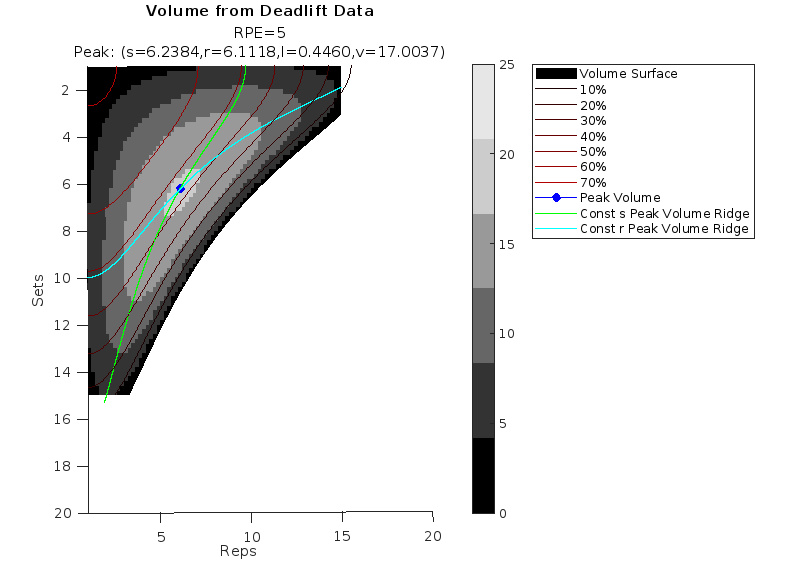
\includegraphics[width=170mm]{DeadliftVolume/FailedRidgeIdentification-2.png}
%    \caption{The peak identified in volume given constant $s$ and $r$ values. This may look similar to figure \ref{fig:DeadliftIntensityCriticalPointsOnVolume} but they are two different graphs that were generated from two different approaches.}
%    \label{fig:VolumeConstSRPeak}
%\end{figure}

The above statements make sense in isolation, but when considered together things can contradict each other. If $\epsilon_5<0$, $\epsilon_6=0$, and $\epsilon_7>0$, then  statement $(3)$ states volume is never bounded, but statement $(14)$ states volume is bounded for a specific region. This is the result of looking at a three dimensional problem from two dimensions. While this does create some problems, the above statements are still is able to give some intuition for the problem at hand. Revisiting the example stated previously, it is saying that volume from reps is never bounded, and volume from sets is only bounded over a specific region.

It is tempting to say the bounds in the above statements can be used in practice to limit the lifter from doing to much volume, but just because volume is bounded does not mean it is reasonable. Just because it can be proven that volume has a peak does not prove that the peak volume is attainable. This is a limitation of the model that stems from using linear regression to fit a surface to the data. Linear regression will implicitly extrapolate what amount of volume can be done given the data it has. Extrapolation is a known weakness of linear regression, making its predicted volume sometimes inaccurate.

In theory, $\epsilon_5$, $\epsilon_6$ and $\epsilon_7$ can be limited to being $> 0$ so that volume is never unbounded. These constraints match those those generated in section \ref{sec:PotentialSurfaceAnalysisOfProperty3} and are shown in equation \ref{eq:BasicSurfaceEquation}. In practice this could lead to a lot of scenarios where the model cannot be applied, severely hindering it's usability. To fix this the range of $\epsilon_5$, $\epsilon_6$ and $\epsilon_7$ can be expanded to being $\ge 0$. Doing this makes it so volume could only ever be unbounded when $\epsilon_5=0$, $\epsilon_6=0$ or $\epsilon_7=0$. This removes the complexities of defining ranges over which the potential surface has bounded volume. After all this work, it can safely be stated that equation \ref{eq:BasicSurfaceEquation} does not properly exhibit property 5.

\section{Analysis of Property 6: 1RM Estimations}
\label{sec:PotentialSurface1RMEstimations}

Property 6 is concerned with 1RM estimations, with it defining an acceptable boundary of accuracy. Table \ref{tab:BasicSurface1RMEstimations} and figure \ref{fig:ApproximateVsActual1RMIntensity} show the models predicted 1RM vs the actual weight that was lifted. \footnote{The lifter did not have access to any of the models estimations when the 1RM attempts were performed, removing any bias from the data that would have been present if the lifter was told the models estimates.} It should be clear from this table that the model consistently under-predicts the lifters actual 1RM with an error much greater than $1\%$. The model almost never predicts above $100\%$ intensity, which is required for a new 1RM.
%The only exception was for heeled squat on $9/10/2022$ but even then the model significantly under-predicted the lifters actual performance.

\begin{figure}[htb]
    \centering
    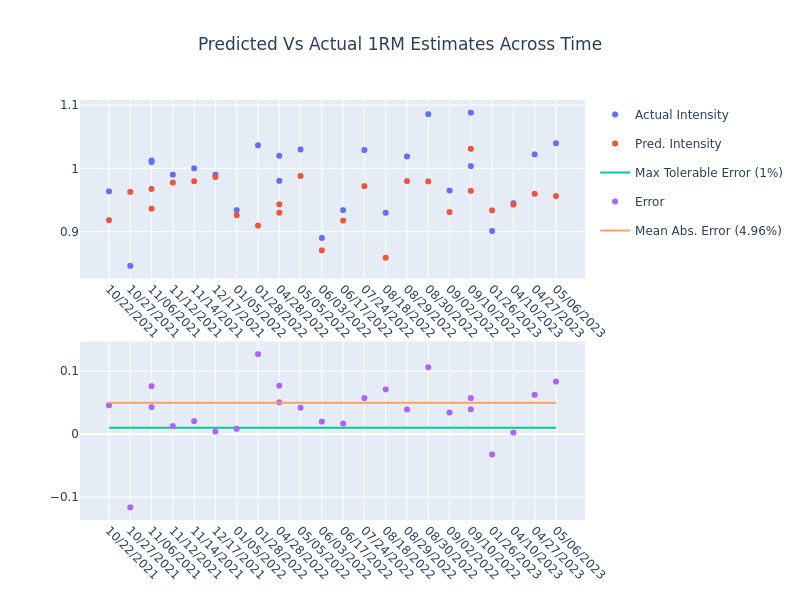
\includegraphics[scale=0.55]{images/ch3/PredVsActual1RM.basic.png}
    \caption{Graphs comparing the approximate and actual 1RM intensity values. Note how the model nearly always under predicts the lifters current 1RM. Of note, though not further discussed until much later, is how the model seems to be getting more accurate as time passes.}
    \label{fig:ApproximateVsActual1RMIntensity}
\end{figure}
\begin{table}[p]
    \centering
	\csvautotabular{../data/generatedData/Client1.1RMPred.slidingWindow.basic.csv}
	\caption{A table showing predicted vs actual 1RM intensities. Note that the model consistently under predicts the lifters current 1RM.}
	\label{tab:BasicSurface1RMEstimations}
\end{table}

There are a couple reasons the model could be exhibiting this behavior. The most prominent however is due to a decision that was made all the way back at the beginning of this chapter. When setting up the $F_{tot}$ equation the terms containing $s$ and $r$ were arbitrarily squared. It is important to note that squaring the terms lead to a better model than if they were left linear, but the choice of squaring the terms was arbitrary. By choosing a power of $2$ the surface was automatically constrained to a certain range of behaviors, and one of the behaviors was how quickly the surface reaches its maximum. Seeing that the model is consistently under-predicting the lifters 1RM, this may be indicative that the surface is leveling off too quick and hence is not able to reach the lifters 1RM appropriately. So what should this constant be? Rather than choosing an arbitrary value, it's value needs to be appropriately chosen from the data, just like the other constants in the surface equation.

\section{Summary}

Before moving forward it is worth quickly noting the success and failures of this surface so that it can be compared to the surfaces presented in the next few chapters. Out of all six properties, this surface exhibited four correctly. The fist property that was not properly exhibited was property 1.b because the surface did not reach a plateau representing the lifters volume tolerance. Despite this hindrance, the surface did seem to exhibit reasonable behavior above $50\%$ intensity, which could make it a viable surface to use as long as this limitation is kept in mind.

Other than property 1.b, property 5 and 6 were also not properly exhibited. Property 5 dealt with unbounded volume. Constraints were placed on the surface limit the occurrence of unbounded volume, but there can still be scenarios where $\epsilon_5=0$, $\epsilon_6=0$, or $\epsilon_7=0$ where unbounded volume can occur. Property 6 was concerned with 1RM estimations. It was shown that the surface consistently under-predicts the lifters 1RM. This is problematic for several reasons, but largely because a lifters goal is to increase there 1RM, making accurate 1RM estimations necessary to track progress. Table \ref{tab:BasicSurfacePropertiesAndBehaviorsSummary} summarizes the properties and whether or not the surface properly exhibited there behavior. It is clear this surface is far from perfect. Chapter \ref{sec:PotentialSurfaceTheVolumeBaseSurface} will attempt to address some of the previously outlined issues with an updated surface.

\begin{table}[htb]
    \centering
    \begin{tabular}{|c|c|c|}
    		\hline
    		Property & Properly Exhibited & Not Properly Exhibited \\
    		\hline
    		1.a & \cmark & \\
    		1.b & & \xmark \\  		
    		2 & \cmark & \\
    		3 & \cmark & \\
    		4 & \cmark & \\
    		5 & & \xmark \\
    		6 & & \xmark \\
    		\hline
    \end{tabular}
    \caption{Properties and whether or not they are exhibited by this surface.}
    \label{tab:BasicSurfacePropertiesAndBehaviorsSummary}
\end{table}


\chapter{Surface 2: The Volume Base Surface}
\label{sec:PotentialSurfaceTheVolumeBaseSurface}

The second surface builds off of the previous chapter by trying to address one of the weaknesses of the basic surface. Namely, the basic surface does not exhibit property 1.b. In order for this new surface to properly exhibit property 1.b a less literal interpretation of the effort-fatigue model is required. To accomplish this the $\hat{-}$ symbol is going to be treated as division instead of subtraction. This will be done in order to create asymptotic behavior on the $I$ axis which will represent the lifters volume base. Doing this however creates another issue of dividing by zero when total fatigue is zero, requiring a second change. Another constant will be added, $\epsilon_8$, which will be constrained to being $\ne F_{tot}$ to prevent any scenarios where division by zero would occur. The final change is to square intensity, again to make it so volume will exhibit asymptotic behavior on the $I$ axis.\footnote{Confused as to why this is needed? This will be discussed in section \ref{sec:VolumeBasePotentialSurfaceProperty5}.} Equation \ref{eq:VolumeBaseSurfaceEquation} shows the the volume base equation.
 
\begin{equation}
	I^2 = \frac{E_{tot}}{\epsilon_8+F_{tot}}= \frac{
		\epsilon_1E
	}{
		\epsilon_8+
		\epsilon_2 F_l+
		\epsilon_3 F_w+
		\epsilon_4 F_e+
		\epsilon_5 (s-1)^2(r-1)^2+
		\epsilon_6 (s-1)^2+
		\epsilon_7 (r-1)^2
	}
	\label{eq:VolumeBaseSurfaceEquation}
\end{equation}

It is worth noting that this surface does not contain an error term, $\epsilon$, like the basic surface. If it did the constants in the equation would no longer be separable and linear regression could not be performed. Even as the equation stands, some algebraic manipulation will need to be performed before linear regression can be performed. In order to make equation \ref{eq:VolumeBaseSurfaceEquation} usable with linear regression its inverse will need to be found, and linear regression will be run on the inverse of intensity. Taking the inverse of equation \ref{eq:VolumeBaseSurfaceEquation} results in the equation shown below which linear regression can be run on.

\begin{minipage}{\textwidth}
	\begin{equation*}
		\frac{1}{I^2}=
			\epsilon_{8,N}\frac{1}{E}+
			\epsilon_{2,N}\frac{F_l}{E}+
			\epsilon_{3,N}\frac{F_w}{E}+
			\epsilon_{4,N}\frac{F_e}{E}+
			\epsilon_{5,N}\frac{(s-1)^2(r-1)^2}{E}+
			\epsilon_{6,N}\frac{(s-1)^2}{E}+
			\epsilon_{7,N}\frac{(r-1)^2}{E}
	\end{equation*}
	\centerline{where}
		\begin{equation*}
			\epsilon_{i\in\{2,3,...,8\},N}=
			\frac{\epsilon_i}{\epsilon_1}
	\end{equation*}
\end{minipage}

At this point an error term could be added, and it would likely make the results from linear regression better, but doing this would change the meaning of equation \ref{eq:VolumeBaseSurfaceEquation} in such a way that it would no longer follow the effort-fatigue model. The result of adding an error term and solving back to match the form of equation \ref{eq:VolumeBaseSurfaceEquation} is shown below. This equation has relationships between $F_{tot}$ and $E_{tot}$ that are not present in the effort-fatigue model. For this reason, an error term will not be added.

\begin{equation*}
	I^2=\frac{
		\epsilon_1E
	}{
		\epsilon\epsilon_1E
		\epsilon_8+
		\epsilon_2 F_l+
		\epsilon_3 F_w+
		\epsilon_4 F_e+
		\epsilon_5 (s-1)^2(r-1)^2+
		\epsilon_6 (s-1)^2+
		\epsilon_7 (r-1)^2
	}=\frac{E_{tot}}{\epsilon E_{tot}+F_{tot}}
\end{equation*}

Throughout the rest of this chapter only the $\epsilon_{i\in\{2,3,...,8\},N}$ constants will be used. There is no need to keep the original constants as they provide no intuitive meaning beyond what can already be found in the new constants. As such, these new constants will simply replace the old constants in notation and be referred to as $\epsilon_{i\in\{2,3,...,8\}}$. The old constants will not be used. With this, the final equation for the volume base surface is shown in equation \ref{eq:VolumeBaseSurfaceEquationInverse}.

\begin{minipage}{\textwidth}
	\begin{equation}
		\frac{1}{I^2}=
			\epsilon_{8}\frac{1}{E}+
			\epsilon_{2}\frac{F_l}{E}+
			\epsilon_{3}\frac{F_w}{E}+
			\epsilon_{4}\frac{F_e}{E}+
			\epsilon_{5}\frac{(s-1)^2(r-1)^2}{E}+
			\epsilon_{6}\frac{(s-1)^2}{E}+
			\epsilon_{7}\frac{(r-1)^2}{E}
		\label{eq:VolumeBaseSurfaceEquationInverse}
	\end{equation}
	\centerline{where}
	\begin{equation*}
		\begin{split}
	        E & \in \{ 1,1.5,2,2.5, \dots ,10 \} \\
	        \epsilon_2, \epsilon_3, \epsilon_4, \epsilon_5,\epsilon_6,\epsilon_7, \epsilon_8 & > 0 \\
	    \end{split}
	\end{equation*}
\end{minipage}\\

Linear regression can now be run with this equation. The error equation that needs to be minimized is shown below.

\begin{equation*}
	E_{rr}=\sum_{
            \substack{i=0\\ t_i\in \{ T \}}
        }^n \left(
        \frac{1}{I_i^2}
        -\epsilon_8 \frac{1}{E_i}
        -\epsilon_2 \frac{F_{l,i}}{E_i}
        -\epsilon_3 \frac{F_{w,i}}{E_i}
        -\epsilon_4 \frac{F_{e,i}}{E_i}
        -\epsilon_5 \frac{(s_i-1)^2(r_i-1)^2}{E_i}
        -\epsilon_6 \frac{(s_i-1)^2}{E_i}
        -\epsilon_7 \frac{(r_i-1)^2}{E_i}
    \right)^2
\end{equation*}

To minimize the error, the partial derivatives of each unknown constant need to be found and each one set equal to zero. An example with $\epsilon_8$ is shown below.

\begin{equation*}
    \begin{split}
        \frac{\partial E_{rr}}{\partial \epsilon_8}=
        \frac{\partial}{\partial \epsilon_8}\sum_{
                \substack{i=0\\ t_i\in \{ T \}}
            }^n \left(
            \frac{1}{I_i^2}
            -\epsilon_8 \frac{1}{E_i}
            +\epsilon_2 \frac{F_{l,i}}{E_i}
            +\dots
            +\epsilon_6 \frac{(s_i-1)^2}{E_i}
            +\epsilon_7 \frac{(r_i-1)^2}{E_i}
        \right)^2&=0
        \\
        -2\sum_{
                \substack{i=0\\ t_i\in \{ T \}}
            }^n \left(
            \frac{1}{I_i^2}
            -\epsilon_8 \frac{1}{E_i}
            -\epsilon_2 \frac{F_{l,i}}{E_i}
            -\dots
            -\epsilon_6 \frac{(s_i-1)^2}{E_i}
           	-\epsilon_7 \frac{(r_i-1)^2}{E_i}
        \right)\left( \frac{1}{E_i} \right)&=0 
        \\
        \epsilon_8 \sum_{\substack{i=0\\ t_i\in \{ T \}}}^n \frac{1}{E_i^2} 
        +\epsilon_2 \sum_{\substack{i=0\\ t_i\in \{ T \}}} \frac{F_{l,i}}{E_i}
        +\dots
        +\epsilon_6 \sum_{\substack{i=0\\ t_i\in \{ T \}}}^n \frac{(s_i-1)^2}{E_i}
        +\epsilon_7 \sum_{\substack{i=0\\ t_i\in \{ T \}}}^n \frac{(r_i-1)^2}{E_i}
        &=
        \sum_{\substack{i=0\\ t_i\in \{ T \}}}^n \frac{1}{I_i^2E_i}
        \\
    \end{split}
\end{equation*}

After a similar process is carried out for each unknown constant, equation \ref{eq:VolumeBaseLinearRegMatrixEquation} can be used, and the unknown constants can be solved for.

\begin{equation}
    \label{eq:VolumeBaseLinearRegMatrixEquation}
	\left[
    \begin{matrix}
        \sum_{i=0}^n \frac{1}{E_i^2} &
        \dots &
        \sum_{\substack{i=0\\ t_i\in \{ T \}}}^n \frac{(r_i-1)^2}{E_i^2} \\

        \sum_{\substack{i=0\\ t_i\in \{ T \}}}^n  \frac{F_{l,i}}{E_i^2} &
        \dots &
        \sum_{\substack{i=0\\ t_i\in \{ T \}}}^n \frac{F_{l,i}(r_i-1)^2}{E_i^2}\\

        \vdots &
        \ddots &
        \vdots \\
        
        \sum_{\substack{i=0\\ t_i\in \{ T \}}}^n \frac{(r_i-1)^2}{E_i^2} &
        \dots &
        \sum_{\substack{i=0\\ t_i\in \{ T \}}}^n \frac{(r_i-1)^4}{E_i^2}
    \end{matrix}
    \right]
    \left[
    \begin{matrix}
        \epsilon_8 \\ \epsilon_2 \\ \vdots \\ \epsilon_7
    \end{matrix}
    \right]
    =
	\left[
    \begin{matrix}
        \sum_{\substack{i=0\\ t_i\in \{ T \}}}^n \frac{1}{I_i^2E_i} \\
        \sum_{\substack{i=0\\ t_i\in \{ T \}}}^n \frac{F_{l,i}}{I_i^2E_i} \\
        \vdots \\
        \sum_{\substack{i=0\\ t_i\in \{ T \}}}^n \frac{(r_i-1)^2}{I_i^2E_i}  
    \end{matrix}
    \right]
\end{equation}

With equations \ref{eq:VolumeBaseSurfaceEquation}- \ref{eq:VolumeBaseLinearRegMatrixEquation} the surface is fully defined and can be fitted to the data presented in chapter \ref{sec:DataSection}. Equation \ref{eq:VolumeBaseIntensitySubedInVolume} shows the result of solving the potential surface for $I$ and substituting it in equation \ref{eq:IntensityBasedVolumeEquation}. Figure \ref{fig:VolumeBaseSquatPotentialSurfaceAcrossEffort} shows the volume base potential surface and figure \ref{fig:VolumeBaseSquatPotentialSurfaceVolumeAcrossEffort} shows the volume surface generated from this surface.

\begin{equation}
    \label{eq:VolumeBaseIntensitySubedInVolume}
    \begin{split}
    		v = & srI l_{1RM} \\
    			= & l_{1RM} sr \left( 
    			\frac{
    				E
    			}{
    				\epsilon_8+
    				\epsilon_2 F_l+
    				\epsilon_3 F_w+
    				\epsilon_4 F_e+
    				\epsilon_5 (s-1)^2(r-1)^2+
    				\epsilon_6 (s-1)^2+
    				\epsilon_7 (r-1)^2
    			}
    		\right)^{\frac{1}{2}}
    \end{split}
\end{equation}

\begin{figure}[htbp]
    \centering
    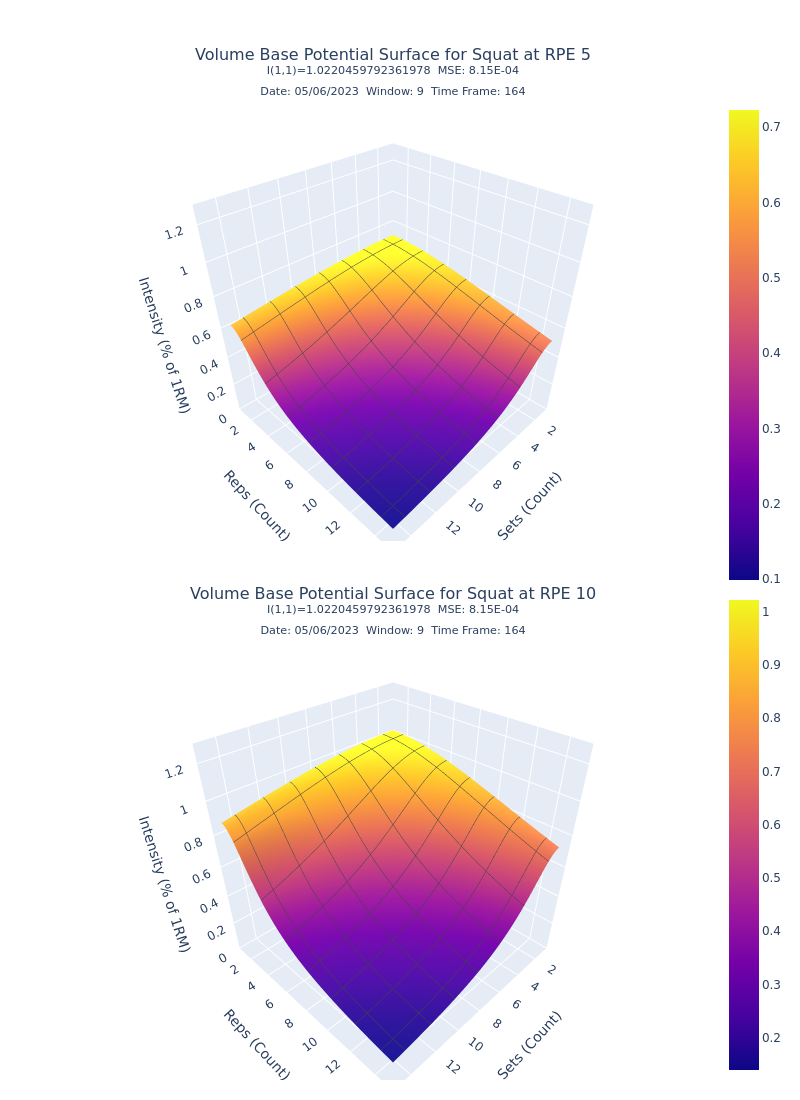
\includegraphics[scale=0.55]{images/ch3/PotentialSurface/DualSquat.Effort[5,10].volumeBase.png}
    \caption{The potential surface fitted to squat data at various effort levels. The window and time frame values will be discussed in chapter \ref{sec:TimeFrame}. For now, the $I(1,1)$ and MSE values are the most important.}
    \label{fig:VolumeBaseSquatPotentialSurfaceAcrossEffort}
\end{figure}

\begin{figure}[htbp]
    \centering
    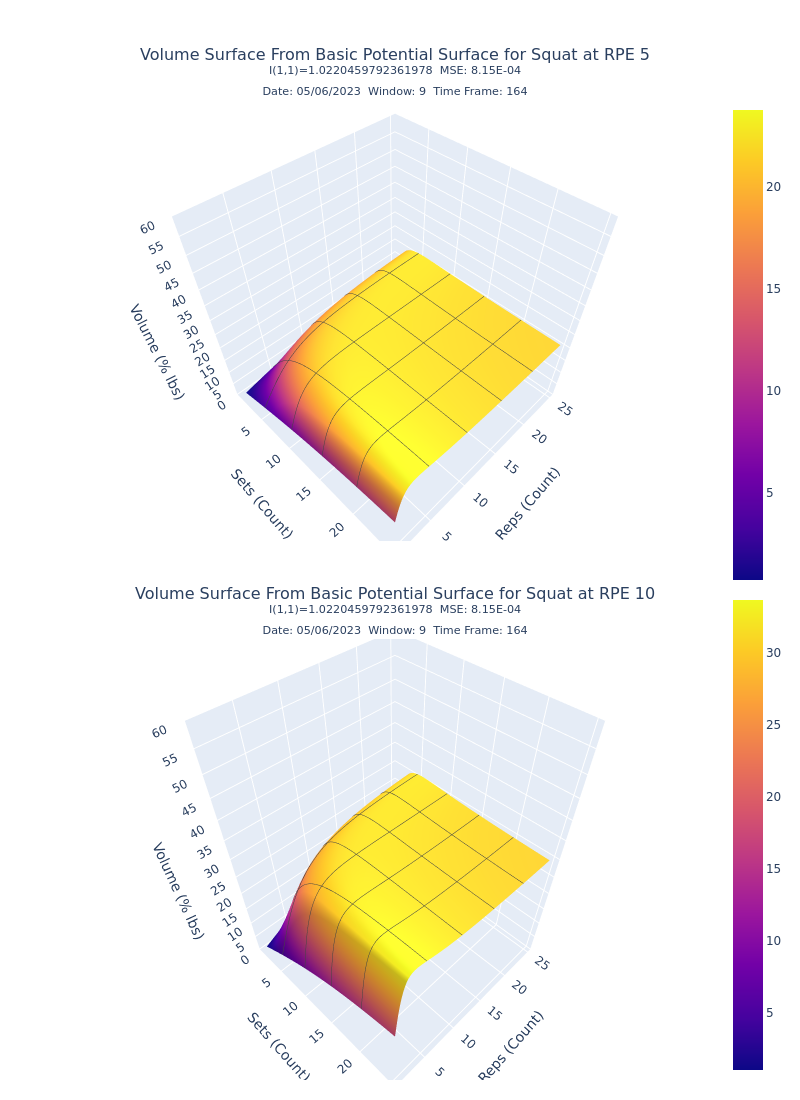
\includegraphics[scale=0.55]{images/ch3/Volume/DualSquat.Effort[5,10].volumeBase.png}
    \caption{The volume surface resulting from the potential surface fitted to squat data at various effort levels.}
    \label{fig:VolumeBaseSquatPotentialSurfaceVolumeAcrossEffort}
\end{figure}

\section{Analysis of Property 1.a: Volume and Intensity}
\label{sec:VolumeBasePotentialSurfaceProperty1a}

Property 1.a states that volume should approach the lifters 1RM as intensity increases given constant effort and fatigue levels. The proof for this will be analogous to the one for the basic surface, where a maximum will be found in the intensity equation at the same point volume will be shown to have a minimum. At this point volume will need to equal intensity. To do this, the gradient of equation \ref{eq:VolumeBaseSurfaceEquation} is needed after it is solved for $I$.

\begin{equation*}
	\begin{split}
		\nabla I & =
		\left[
		\begin{matrix}
		 	\frac{\partial I}{\partial E} \\
			\frac{\partial I}{\partial F_l} \\
			\frac{\partial I}{\partial F_w} \\
			\frac{\partial I}{\partial F_e} \\ 
			\frac{\partial I}{\partial s} \\
			\frac{\partial I}{\partial r} \\
		\end{matrix}
		\right] =
		\left[
		\begin{matrix}
			\frac{1}{2}
			E^{-\frac{1}{2}}
			\left(
				\epsilon_8+
				\epsilon_2 F_l+
    				\epsilon_3 F_w+
    				\epsilon_4 F_e+
    				\epsilon_5 (s-1)^2(r-1)^2+
    				\epsilon_6 (s-1)^2+
    				\epsilon_7 (r-1)^2
    			\right)^{-\frac{1}{2}}
			\\
			-\frac{
				\epsilon_2 E^{\frac{1}{2}}
			}{
				2
			}  \left(
				\epsilon_8+
				\epsilon_2 F_l+
    				\epsilon_3 F_w+
    				\epsilon_4 F_e+
    				\epsilon_5 (s-1)^2(r-1)^2+
    				\epsilon_6 (s-1)^2+
    				\epsilon_7 (r-1)^2
    			\right)^{-\frac{3}{2}}
    			\\
			-\frac{
				\epsilon_3 E^{\frac{1}{2}}
			}{
				2
			}  \left(
				\epsilon_8+
				\epsilon_2 F_l+
    				\epsilon_3 F_w+
    				\epsilon_4 F_e+
    				\epsilon_5 (s-1)^2(r-1)^2+
    				\epsilon_6 (s-1)^2+
    				\epsilon_7 (r-1)^2
    			\right)^{-\frac{3}{2}}
    			\\
			-\frac{
				\epsilon_4 E^{\frac{1}{2}}
			}{
				2
			}  \left(
				\epsilon_8+
				\epsilon_2 F_l+
    				\epsilon_3 F_w+
    				\epsilon_4 F_e+
    				\epsilon_5 (s-1)^2(r-1)^2+
    				\epsilon_6 (s-1)^2+
    				\epsilon_7 (r-1)^2
    			\right)^{-\frac{3}{2}}
    			\\
			\partial_s v
    			\\
			\partial_r v
    			\\
		\end{matrix}
		\right]
		\\
		\partial_s v & =
		-(\epsilon_5+\epsilon_6)(s-1) E^{\frac{1}{2}}
			\left(
				\epsilon_8+
				\epsilon_2 F_l+
    				\epsilon_3 F_w+
    				\epsilon_4 F_e+
    				\epsilon_5 (s-1)^2(r-1)^2+
    				\epsilon_6 (s-1)^2+
    				\epsilon_7 (r-1)^2
    			\right)^{-\frac{3}{2}}
    		\\
    		\partial_r v & =
    		-(\epsilon_5+\epsilon_7)(r-1) E^{\frac{1}{2}}
			\left(
				\epsilon_8+
				\epsilon_2 F_l+
    				\epsilon_3 F_w+
    				\epsilon_4 F_e+
    				\epsilon_5 (s-1)^2(r-1)^2+
    				\epsilon_6 (s-1)^2+
    				\epsilon_7 (r-1)^2
    			\right)^{-\frac{3}{2}}
    		\\
	\end{split}
\end{equation*}

The gradient now needs to be set equal to $0$ and solved for in order to get critical points. One solution to this system of equations is $E=0$. When $E=0$ it does not matter what any of the other variables are, intensity will always be $0$. This behavior matches what would be expected in reality. If the lifter puts no effort they will not be able to lift anything. This result does little in the way of proving property 1.a however, as effort and fatigue are not held constant. If effort and fatigue are held constant and only $\partial_s v$ and $\partial_r v$ are looked at there is another critical point at $(s=1,r=1)$.

\section{Analysis of Property 1.b: Volume and Intensity}
\label{sec:VolumeBasePotentialSurfaceProperty1b}

\section{Analysis of Property 2: Volume and Effort}
\label{sec:VolumeBasePotentialSurfaceProperty2}

It needs to be shown that volume increases with increased effort and decreases with decreased effort. Changes in $v$ in relation to changes to $E$ is required. Solving for the partial derivative of equation \ref{eq:VolumeBaseIntensitySubedInVolume} with respect to $E$ is required.

\begin{equation*}
	\begin{split}
		\frac{\partial v}{\partial E} & =
		\frac{\partial}{\partial E} l_{1RM} sr \left( 
    			\frac{
    				E
    			}{
    				\epsilon_8+
    				\epsilon_2 F_l+
    				\epsilon_3 F_w+
    				\epsilon_4 F_e+
    				\epsilon_5 (s-1)^2(r-1)^2+
    				\epsilon_6 (s-1)^2+
    				\epsilon_7 (r-1)^2
    			}
    		\right)^{\frac{1}{2}}
    		\\
    		& = \frac{
    			l_{1RM} sr
    		}{
    			2 \left(\epsilon_8+F_{tot} \right)^{\frac{1}{2}}
    		} E^{-\frac{1}{2}}
    	\end{split}
\end{equation*}

In order for the desired behavior in effort to be observed, $\partial_E v$ needs to be $>0$. The following constraints are given in section \ref{sec:UnitsOfMeasurement}.

\begin{equation*}
	\begin{split}
		s & \ge 1 \\
		r & \in\{\mathbb{R} \ge 1 \} \\
		w & >0 \\
		E & \in\{1,1.5,2,...,10\}
	\end{split}
\end{equation*}

Given the above constraints and remembering that $l_{1RM}$ is a weight only leaves one term left, the parenthetical grouping on the bottom of the fraction. This term must be positive to satisfy the constraint on $\partial_E v$. Given this, the below statement can be made.

\begin{equation*}
	\frac{
    			l_{1RM} sr
    		}{
    			2 \left(\epsilon_8+F_{tot} \right)^{\frac{1}{2}}
    		} E^{-\frac{1}{2}} >0 \textbf{ iff }\epsilon_8+F_{tot}>0
\end{equation*}

The constraints on the constants that make the parenthetical grouping positive will be discussed in \ref{sec:VolumeBasePotentialSurfaceProperty3}. With these constraints it has been shown that volume increases with increased effort and means the volume base surface properly exhibits property 2.

Before moving on, there are two things of note. The first is that this result did not depend on the sign of any constant, as there was no constant associated with the effort term. This is much different behavior from the basic surface which had to constrain the constant associated with the effort term. The reason for this can be traced all the way back to when the new constants were created to make linear regression possible. When this was done the $\epsilon_1$ constant that was associated with the effort term was absorbed into the new constants, removing the need for any constraint on $\epsilon_1$. However, doing this only moved the problem elsewhere as constraints will now need to be placed on all the constants that absorbed the $\epsilon_1$ constant. As stated previously, this work is done in section \ref{sec:VolumeBasePotentialSurfaceProperty3}.

The second thing of note is how volume increases with increases in effort. To analyze this $\partial_{EE} v$ is needed.

\begin{equation*}
	\partial_{EE}v=-\frac{
    			l_{1RM} sr
    		}{
    			4 \left(\epsilon_8+F_{tot} \right)^{\frac{1}{2}}
    		} E^{-\frac{3}{2}}
\end{equation*}

Since $\partial_{EE}v$ has all the same constants a $\partial_Ev$ it means that $\partial_{EE}v<0$. This means that volume increases with increase effort but it does so with diminishing returns. In other words, a linear increase in effort will cause smaller and smaller increases in volume at higher effort levels. This is very different from the basic surface which had linear increases in volume from linear increases in effort. The question now becomes which one is correct. Fortunately, this does not have to be answered now as the volume base model is actually flexible enough to also represent linear returns to effort. Depending on the scale of the constants from linear regression relative to the finite scale of effort, linear returns can be approximated. Not only does this add an additional layer of flexibility to the volume base model, but it will allow questions related to how volume scales with effort to be answered later in this book.

\section{Analysis of Property 3: Volume and Fatigue}
\label{sec:VolumeBasePotentialSurfaceProperty3}

It needs to be shown that volume decreases with increased fatigue and increases with decreased fatigue. To prove this it will need to be shown that the partial derivatives with respect to every fatigue term are $<0$. Shown below is $\partial_{F_l}v$.

\begin{equation*}
	\begin{split}
		\frac{\partial v}{\partial F_l} & =
		\frac{\partial}{\partial F_l} l_{1RM} sr \left( 
    			\frac{
    				E
    			}{
    				\epsilon_8+
    				\epsilon_2 F_l+
    				\epsilon_3 F_w+
    				\epsilon_4 F_e+
    				\epsilon_5 (s-1)^2(r-1)^2+
    				\epsilon_6 (s-1)^2+
    				\epsilon_7 (r-1)^2
    			}
    		\right)^{\frac{1}{2}}
    		\\
    		& = -\frac{1}{2}
    			\epsilon_2 l_{1RM} sr E^{\frac{1}{2}}
    			\left(
	    			\epsilon_8+
    				\epsilon_2 F_l+
    				\epsilon_3 F_w+
    				\epsilon_4 F_e+
    				\epsilon_5 (s-1)^2(r-1)^2+
    				\epsilon_6 (s-1)^2+
    				\epsilon_7 (r-1)^2
    			\right)^{-\frac{3}{2}}
    	\end{split}
\end{equation*}

Given the same set of constraints placed on $s$, $r$, $w$, and $E$  that was presented in the previous section it should be clear that there are only two terms that can change the sign of the partial derivative: the $\epsilon_2$ constant and the entire parenthetical grouping. The even root on the parenthetical grouping will technically guarantee that term is positive, but in order to make this proof more robust to future changes an alternative proof will be used.

At this point a more formal approach is needed when selecting the constraints on the constants. Unlike the basic surface, many sets of values can be used as the constraints. As such, the best set of values needs to be chosen. The problem can be restated to finding the loosest set of constraints on the constants that still ensures the proper behavior. In mathematical terms it could be restated as the following.

\begin{minipage}{\textwidth}
	\begin{equation*}
		\max v_{\epsilon_1,\epsilon_2,...,\epsilon_8}
		\textbf{ st }
		\left( 
			\min \epsilon_8+\mathbf{\hat{\epsilon}\hat{x}} >0
			\land
			\epsilon_{2,3,...,8}>0
		\right)
		\lor
		\left( 
			\max \epsilon_8+\mathbf{\hat{\epsilon}\hat{x}} <0
			\land
			\epsilon_{2,3,...,8}<0
		\right)
	\end{equation*}
	\centerline{where}
	\begin{equation*}
		\begin{split}
			\max v_{\epsilon_1,\epsilon_2,...,\epsilon_8} &
			\text{ is the volume of the space generated by the constraints}
			\\
			\mathbf{\hat{\epsilon}} & =\left[
				\begin{matrix}
					\epsilon_2 &
					\epsilon_3 &
					\epsilon_4 &
					\dots &
					\epsilon_7
				\end{matrix}
			\right]
			\\
			\mathbf{\hat{x}} & =\left[
				\begin{matrix}
					F_l &
					F_w &
					F_e &
					\dots &
					(s-1)^2(r-1)^2
				\end{matrix}
			\right]^T
	    \end{split}
	\end{equation*}
\end{minipage}\\

Forcing the minimum of $\epsilon_8+\mathbf{\hat{\epsilon}\hat{x}}$ to be $>0$ forces the parenthetical grouping to be positive for all values, which also requires all the constants to be $>0$ to ensure the partial derivative remains $<0$. Forcing the maximum of $\epsilon_8+\mathbf{\hat{\epsilon}\hat{x}}$ to be $<0$ forces the parenthetical grouping to be negative for all values\footnote{This is assuming the root on the parenthetical grouping allows for negative values.}, which also requires all the constants to be $<0$ to ensure the partial derivative remains $<0$.

Before moving on, a brief discussion about why the constants cannot have mixed signs is required. Having mixed signs would violate the constraint on the minimum value of $\epsilon_8+\mathbf{\hat{\epsilon}\hat{x}}$. No matter what values are chosen for the constants, if they are not all positive the negative term(s) can outweigh all the other positive terms given the appropriate values for $\mathbf{\hat{x}}$ and force $\epsilon_8+\mathbf{\hat{\epsilon}\hat{x}}<0$. Of note is that if $\epsilon_8+\mathbf{\hat{\epsilon}\hat{x}}$  is allowed to be negative then there is not only no minimum, but any minimum that could potentially exist would be $<0$. The exact same argument could be made for how the constraint on the maximum value of $\epsilon_8+\mathbf{\hat{\epsilon}\hat{x}}$ would be violated, just with positive and negative values switching places. As such, any solution containing mixed signs is not a valid solution.

Looking at the equation presented above, the solutions are already present. The solutions are where the constants are either all positive or all negative. Any solution other than those two solutions would unnecessarily limit the volume of space generated by the constants. The question now becomes which solution is the right one, as both solutions take up equal volume from the space generated by the constants. The detail that chooses which solution to use comes down to the sign of $v$ and $I$. If $\epsilon_{2,3,...,8}$ are all $<0$ then $v<0$ and $I<0$, which does not make sense from the context of the problem. Negative intensity does not make sense because that would imply negative weight and the same argument applies to volume. This limits the solution to $\epsilon_{2,3,...8}>0$.

With it being proven that $\epsilon_{2,3,...,8}>0$ maximizes the volume of space generated by the constraints while preserving the correct behavior, it can be stated that the volume base surface properly exhibits property 3. Just like the previous section, further analysis can be done that looks at how volume decreases from increases in fatigue. Again, this needs to be done for every term in $F_{tot}$. Shown below is $\partial_{F_lF_l}v$.

\begin{equation*}
	\partial_{F_lF_l}v=
		\frac{3}{4}
    		\epsilon_2^2 l_{1RM} sr E^{\frac{1}{2}}
    		\left(
	    		\epsilon_8+
    			\epsilon_2 F_l+
    			\epsilon_3 F_w+
    			\epsilon_4 F_e+
    			\epsilon_5 (s-1)^2(r-1)^2+
    			\epsilon_6 (s-1)^2+
    			\epsilon_7 (r-1)^2
    		\right)^{-\frac{5}{2}}
\end{equation*}

Just like the previous section, the second partial derivative changed sign relative to the first partial derivative. In this case it means that volume decreases with diminishing returns to increases in fatigue. \footnote{Having a linear increase in fatigue represent a sub-linear decrease in volume can have some very important implications when it comes to planning deloads for lifters. It could be said that this is why lifters make progress, as a lifter would not have to linearly decrease volume to where they were previously every time fatigue is high, allowing for incremental increases in total volume over time.} Also just like the last section, linear returns can be approximated.

\section{Analysis of Property 4: Sets and Reps}
\label{sec:VolumeBasePotentialSurfaceProperty4}

\section{Analysis of Property 5: Bounded Volume}
\label{sec:VolumeBasePotentialSurfaceProperty5}

\section{Analysis of Property 6: 1RM Estimations}
\label{sec:VolumeBasePotentialSurfaceProperty6}

\section{Summary}

\chapter{
    Time Frame
    \\
    \large{Fine Tuning The Model}
}
\label{sec:TimeFrame}

Section \ref{sec:PotentialSurfaceLinearRegressionAndTimeSeriesProblems} introduced the notion of a time frame, or a window of time over which data is selected to use for linear regression. This is important because it allows the model to track changes over time. The natural question then becomes how long should the time frame be, and is what this section is concerned with.

Figure \ref{fig:Pred1RMMultipleTimeFrames} shows how the predicted 1RM changes over time with varying time frames. It should be clear that the time frame chosen has a significant impact on what predictions the model makes, and as such will need to be chosen so that it increases the accuracy of the model. This will require first defining the models accuracy, and then later using that definition to choose a time frame such that the models accuracy is maximized.

\begin{figure}[h]
    \centering
    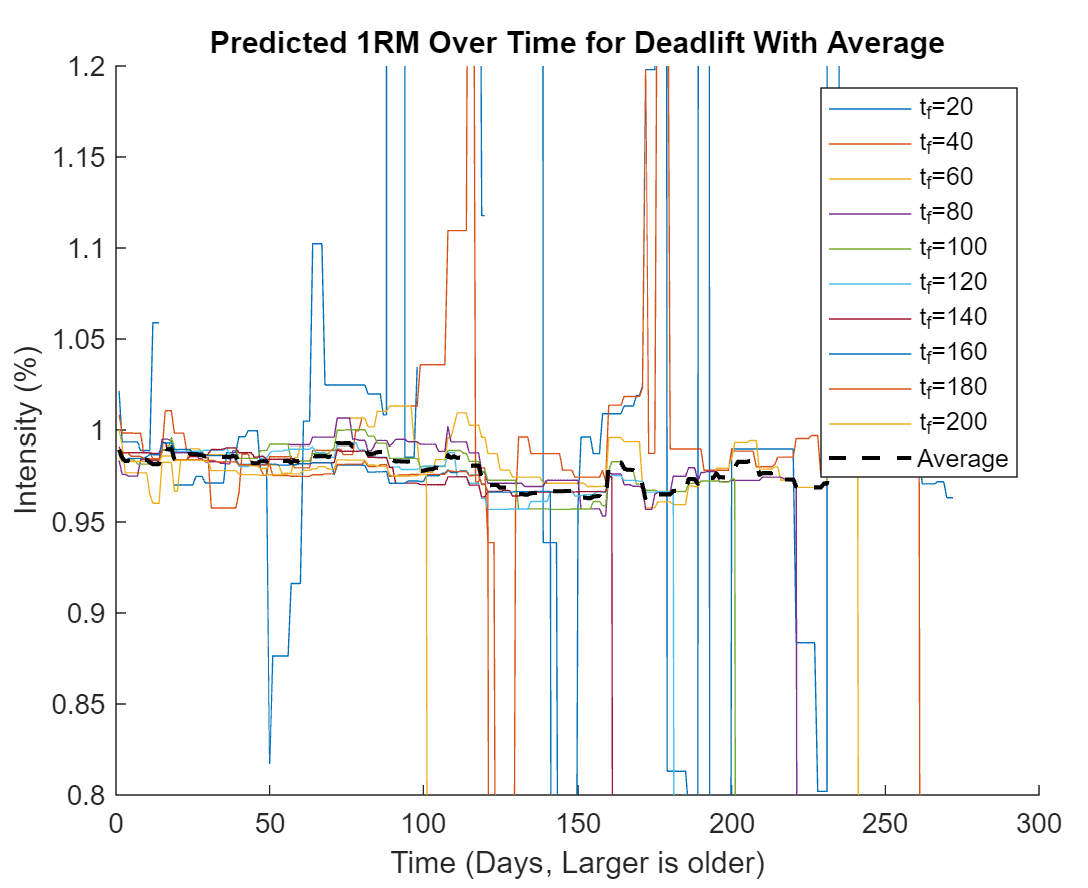
\includegraphics{DeadliftConstants/pred1RMMultipleTimeFrames.png}
    \caption{The models predicted 1RM over varying time frames. The large spikes and dips are from the model not having enough data to fit the fatigue aware potential surface to. The $20$ and $40$ time frames were excluded from calculating the average due to there erratic and inaccurate behavior.}
    \label{fig:Pred1RMMultipleTimeFrames}
\end{figure}

\section{Establishing Lose Bounds}
\label{sec:TimeFrameEstablishingLooseBounds}

The first thing to take note of from figure \ref{fig:Pred1RMMultipleTimeFrames} is the $20$ and $40$ day time frames, as they have large spikes and drops. This is the result of the model not having enough data. Given that the lifter performed deadlifts at most $2$ times a week, this creates a maximum of $11$ data points for linear regression to use over a $40$ day time frame. This is not enough data for the model to accurately predict anything. The time frame chosen needs to be large enough for the model to have enough data to reliably create predictions. With this in mind, the 1RM prediction has presented itself as a proxy to determine if the model was given enough data. If the 1RM prediction is within 'reasonable' bounds then it can be presumed that the model was given enough data to make accurate predictions. This is not an exact measurement to determine if the model has been given enough data, but is a proxy that can help avoid situations where the model was clearly not given enough data.

Looking at the larger time frames the behavior is much more stable, but at the cost of requiring more data to create any predictions. If a time frame is to large it will fail to adapt to recent changes in a lifters abilities, as it includes old data that may no longer be relevant to a lifters current capabilities. It should be clear that when considering a time frame, a balance needs to be struck so that the model has enough data to be reliable but not to much data so that it fails to capture recent changes in a lifters abilities.

\section{Accuracy: Defining State and What is Being Measured}
\label{sec:TimeFrameWhatIsBeingMeasured}

The 1RM prediction has already been introduced as a measure of accuracy in sections \ref{sec:PotentialSurfaceSolvingForTheUnknown}, \ref{sec:PotetentialSurfaceImprovingAccuracy}, and just now in section \ref{sec:TimeFrameEstablishingLooseBounds}. However, this is only a single data point from the output of the model. Accuracy can, and probably should, be considered in a much larger context. From equations \ref{eq:PotentialSurfaceSetsEquationWithFatigue}-\ref{eq:PotentialSurfaceFatigueEquation}, it can be presumed that the model can predict sets, reps, effort, intensity, and fatigue.

\begin{wrapfigure}{l}{0.55\textwidth}\centering
    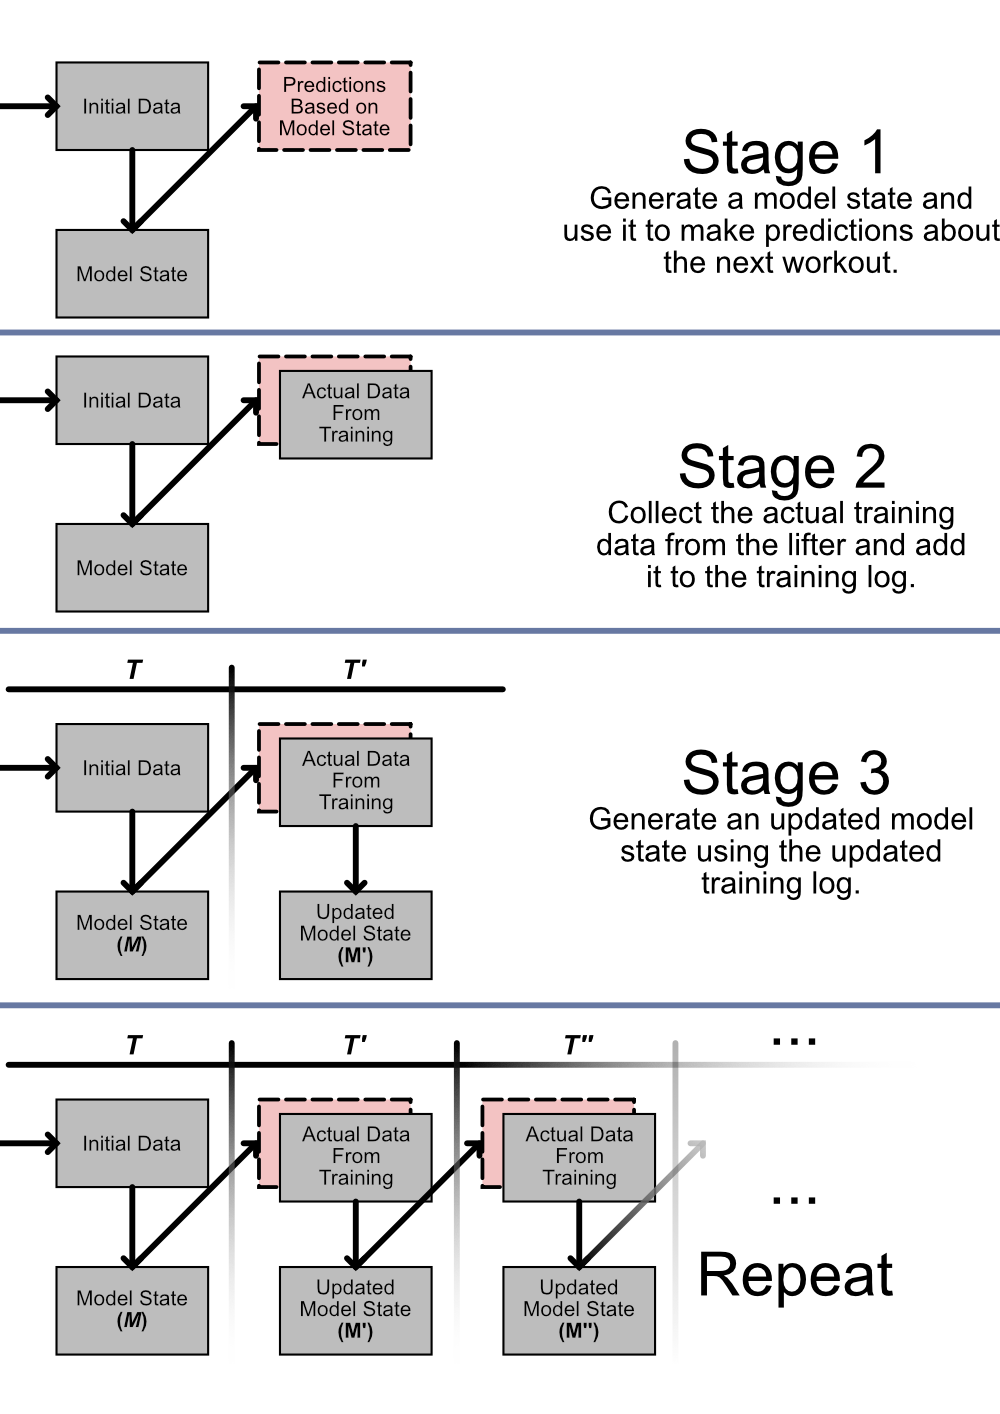
\includegraphics[width=95mm]{Diagrams/PredictionsDiagram.png}
    \caption{A diagram showing how the model makes predictions through time.}
    \label{fig:ModelPredictionsDiagram}
\end{wrapfigure}

Before any discussion about measuring accuracy, it is worth describing how the model predicts values. If the model is predicting a value for the current day, then it will use historical data that is within the selected time frame, $t_i\in\{ t_t=t_0, t_t+1=t_0+1, \dots, t_0+t_f \}$, to create a prediction. Given this specific set of historical data, the model will have a certain state, called the \textit{model state}, which is defined by the set of all constants produced from linear regression, as shown in equation \ref{eq:ModelState}. This definition makes the model state specific to the subset of historical data used, hence the $T$ subscripts, and means that the state of the model will change with any changes to the time frame. This is consistent with the observations made from figure \ref{fig:Pred1RMMultipleTimeFrames}.

\begin{equation}
    \label{eq:ModelState}
    M\in \{ a_{T}, b_{T}, c_{T}, \epsilon_{T}, \epsilon_{2,T} \}
\end{equation}

Once the actual data for a given day is added to the data set, any discrepancies between the predicted and actual data can be used to measure accuracy. When the lifter goes to train the next time, the process can repeat itself all over again, but this time the model will use time frame $T'$ and will be in in state $M'$ because of the data that was added from the previous workout. It is through this mechanism that the model is able to change state as it moves through time, and gives it the ability to adapt to represent the lifters current abilities. Figure \ref{fig:ModelPredictionsDiagram} demonstrates this process in a graphical manner.

The above process of the model updating state as it moves through time is necessary for the model to adapt, but creates challenges when attempting to gather historical data, which can be used to do things like measure accuracy over time. Every time a prediction needs to be made for time $t_t$, the model must use the appropriate time frame to get the state of the model before the data at time $t_t$ was added. Calculating the models state is a non-trivial process, and having to repeat it for every time value results in large computational overhead. Any efficiency that can be gained from calculating the models state will have significant impacts on the speed of generating historical model data.

Now that it is known how the model makes predictions, and hence how to measure accuracy, tools like the mean square error (MSE) and root mean square error (RMSE) can be used to measure accuracy from a larger context. The graphs in table \ref{tab:PredictionsVsActualConstantTimeFrame} show the actual vs predicted values for various variables using deadlift data. The reason there are not predictions for all values is because some values were to close to the end of the data set for the given time frame to make predictions, which brings up an important point: the amount of data the model needs before it can start creating predictions is dependent on the time frame chosen. This limitation will be partially removed in section \ref{sec:TimeFrameDynamicTimeFrameAnalysis}, but cannot be wholly removed because the model will always need a certain amount of data to create reliable predictions, as discussed in section \ref{sec:TimeFrameEstablishingLooseBounds}.

\begin{table}
    \centering
    \begin{tabular}{c|c}
        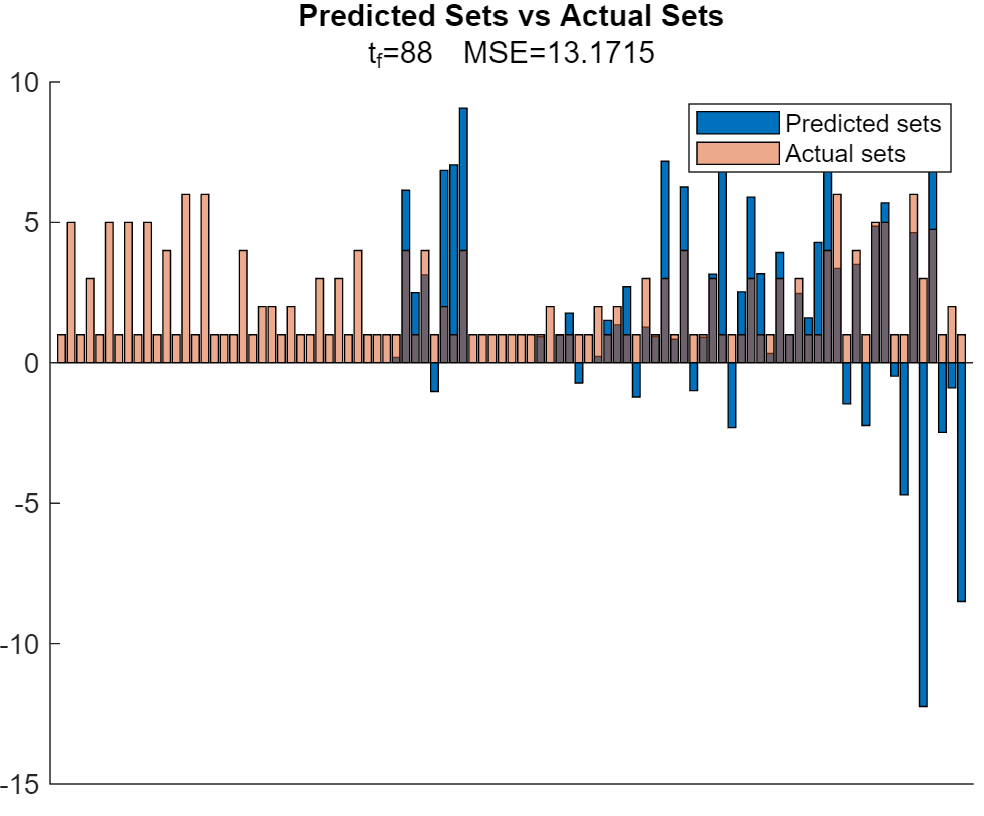
\includegraphics[width=80mm]{ActualVsPredValues/ActualVsPredSets.png} &
        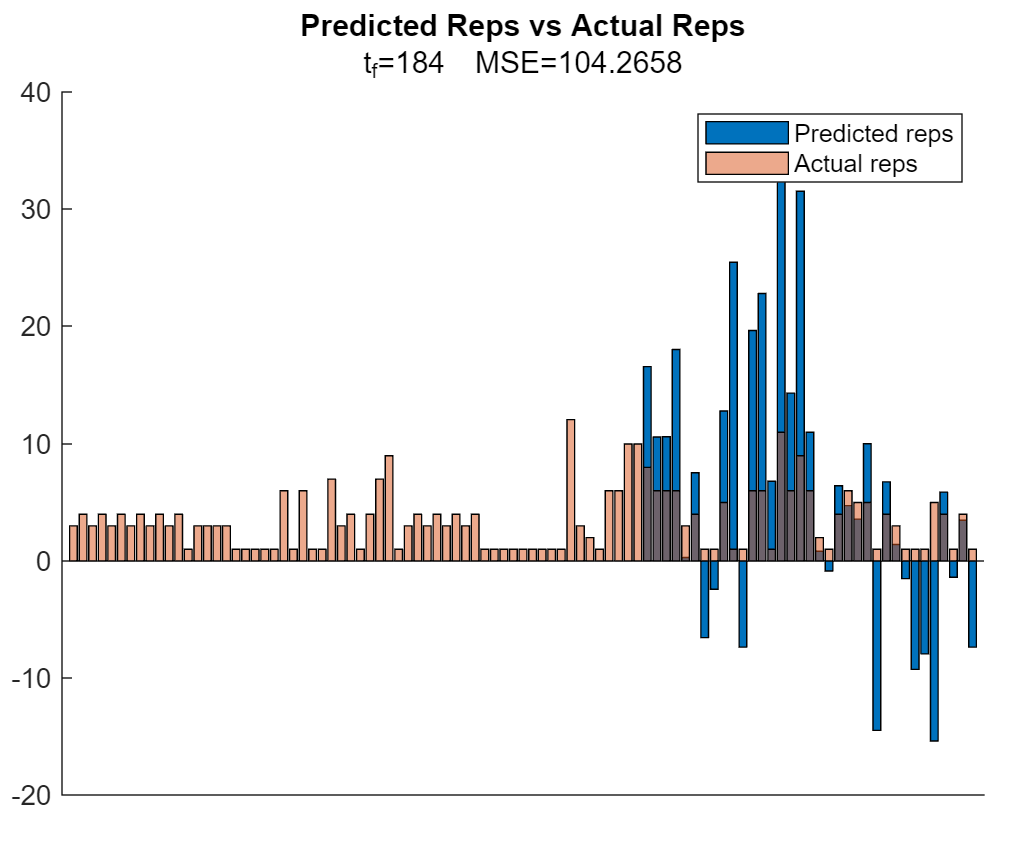
\includegraphics[width=80mm]{ActualVsPredValues/ActualVsPredReps.png}  \\
        
        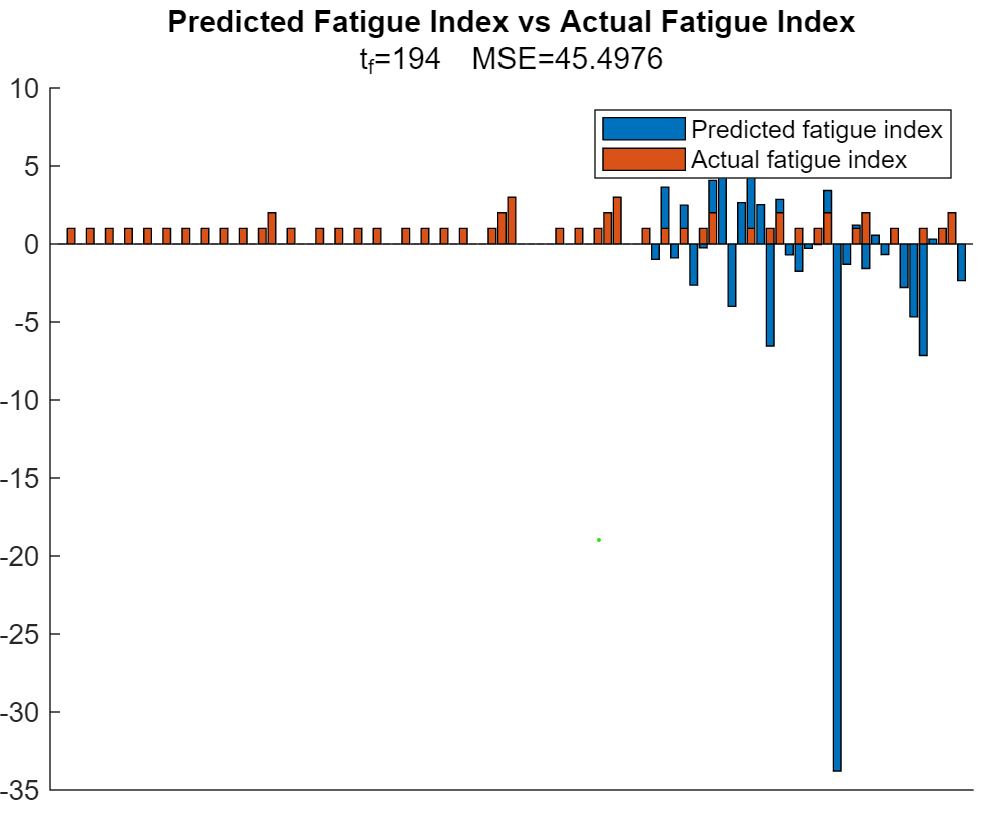
\includegraphics[width=80mm]{ActualVsPredValues/ActualVsPredFatigueIndex.png} &
        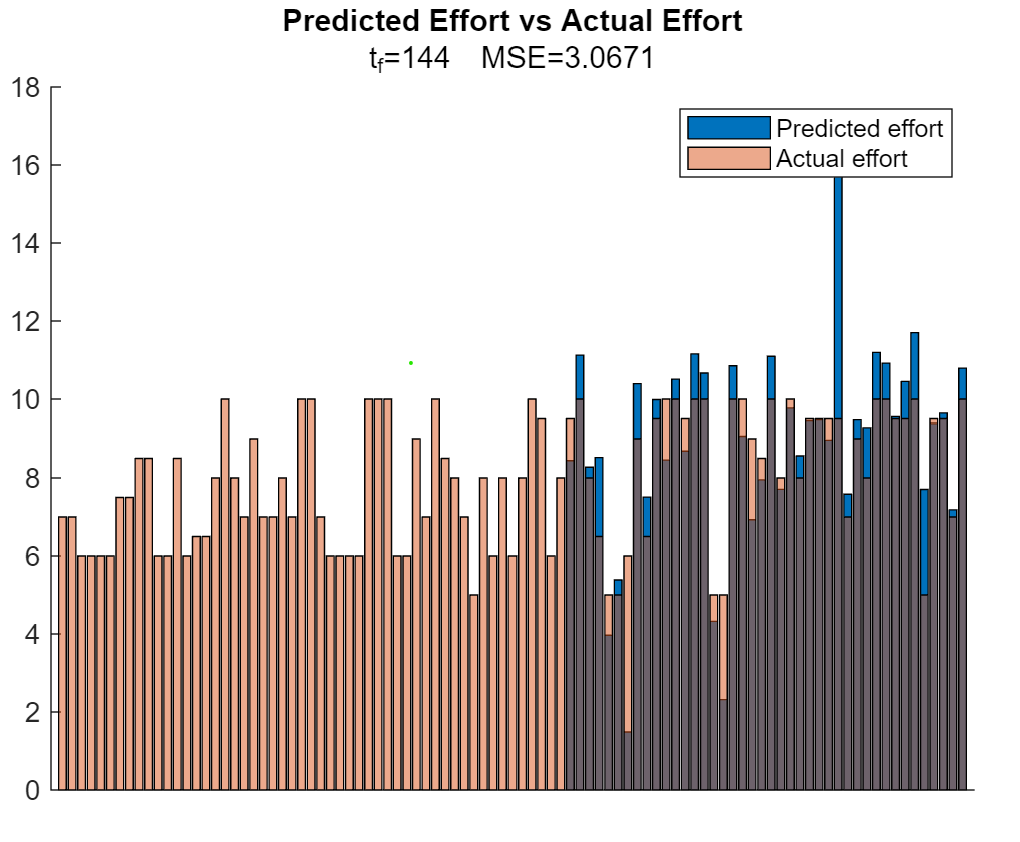
\includegraphics[width=80mm]{ActualVsPredValues/ActualVsPredEffort.png} \\
        
        \multicolumn{2}{c}{
            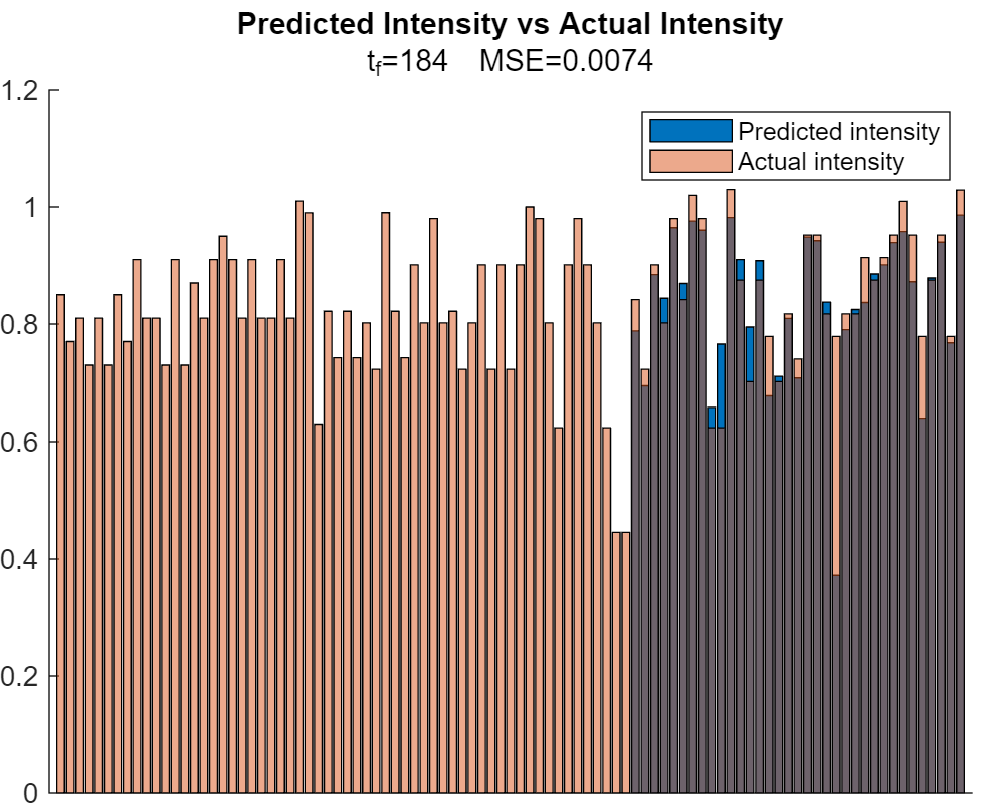
\includegraphics[width=100mm]{ActualVsPredValues/ActualVsPredIntensity.png}
        }
    \end{tabular}
    \caption{Predicted values compared to actual values for various variables using deadlift data. Sets, reps, and the fatigue index are not accurate, but effort is more accurate, and intensity is very accurate. The MSE was calculated only using data points that had a predicted value.}
    \label{tab:PredictionsVsActualConstantTimeFrame}
\end{table}

Some of the graphs from table \ref{tab:PredictionsVsActualConstantTimeFrame} may seem surprising, especially the ones relating to sets, reps, and the fatigue index. The results displayed in these graphs are highly inaccurate. The reason for this is rather simple, in section \ref{sec:PotentialSurfaceDefiningTheRelationships} the error terms that were minimized were in relation to intensity, which defined intensity as the dependent variable. Even before that however, the intuitive relationships discussed in section \ref{sec:PotentialSurfaceIntuitiveRelationshipsBetweenVariables} were all focused on how volume, effort, sets, and reps all affected intensity, which implicitly defined all of those values as independent variables and intensity the dependent variable. So, the reason for the inaccuracy in the set, rep, and fatigue index graphs are because a dependent variable was being predicted from an independent variable, which in the context of modeling does not make sense. This also explains the accuracy of the intensity graph, with the predicted intensity, on average, being within $0.74\%$ of the actual intensity. Moving forward, this means that equations \ref{eq:PotentialSurfaceSetsEquationWithFatigue}, \ref{eq:PotentialSurfaceRepsEquationWithFatigue}, \ref{eq:PotentialSurfaceEffortEquationWithFatigue}, and \ref{eq:PotentialSurfaceFatigueEquation} should all be used sparingly, and when used there results should be questioned. Of note is that equation \ref{eq:1RMPredictionWithFatigue} remains unaffected by this, and means that the 1RM predictions produced by the model should have some accuracy to them.

\section{Choosing A Time Frame: Static Time Frame Analysis}
\label{sec:TimeFrameStaticTimeFrameAnalysis}

A time frame of constant length $t_f$ can be used across all time values to generate predictions, creating a 'static time frame'. With accuracy defined and having shown how the model predicts values, the MSE of intensity across all time values can be used as a way to select a value for $t_f$ that maximizes the accuracy of the model. Figure \ref{fig:StaticTimeFrameDiagram} demonstrates the process of selecting a static time frame.

\begin{figure}[h]
    \centering
    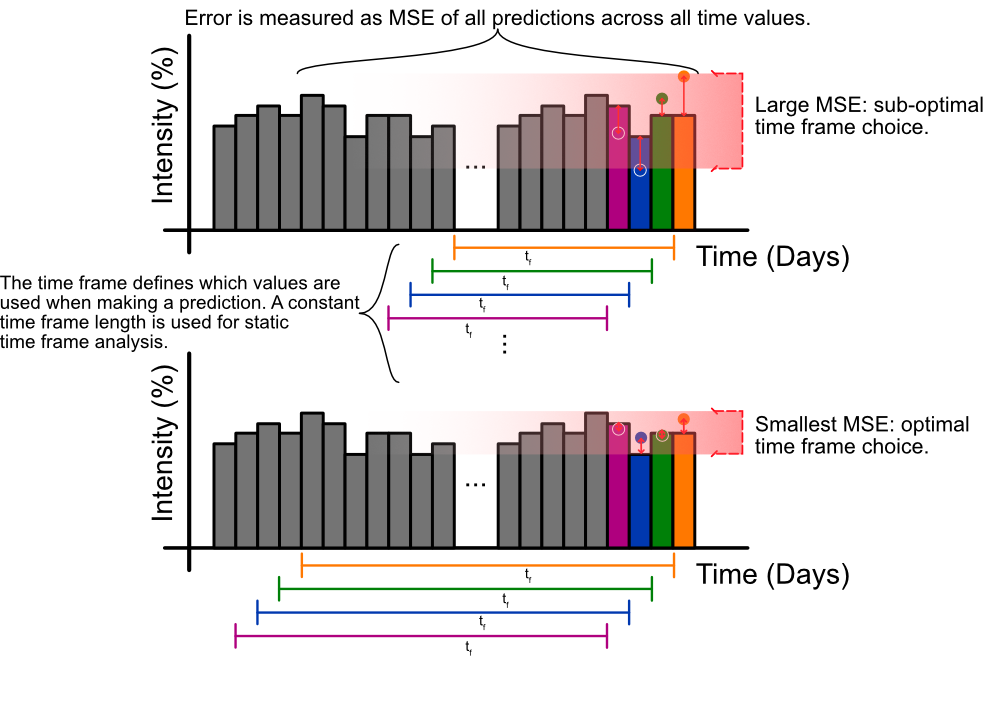
\includegraphics[width=150mm]{Diagrams/StaticTimeFrameDiagram.png}
    \caption{A diagram showing how a static time frame is calculated from the data set. Note how the predictions for all time values need to be recalculated.}
    \label{fig:StaticTimeFrameDiagram}
\end{figure}

The models accuracy will be maximized when the MSE is minimized. In order to find the global minimum MSE, all valid values of $t_f$ must be tested and there respective MSE's calculated. Equation \ref{eq:ValidTimeFrameSet} shows the set that determines all valid values for the time frame given a target time, $t_t$.

\begin{equation}
    \label{eq:ValidTimeFrameSet}
    t_f \in \{ 0, 1, \dots , \max_{t_1\dots t_n}( t )-t_t \}
\end{equation}

The algorithm shown in listing \ref{lst:StaticTimeFrameFormula} can be used to find the $t_f$ value where the MSE is minimized. Given that \texttt{modelState} runs in linear time with it's arguments, which happens because it has to sum up values across it's given time frame, this algorithm has a time complexity of $O(n^3)$. As the lifter keeps lifting and the data set grows $\max_{t_1\dots t_n}(t)$ will continually increase, eventually making an exhaustive search of all $t_f$ values infeasible. An analytical approach to finding the global minimum of the MSE would be nice, but this is not possible as the MSE error function is not a continuous function rendering any method derived from calculus useless. If historical data is needed, the time complexity gets even worse, with listing \ref{lst:HistoricalStaticTimeFrameFormula} showing the that the time complexity of getting historical data is $O(n^4)$.

% \begin{equation}
%     \sum_{t_f\in\{0,1,...,\max_{t_1...t_n}(t)\}}\left(
%         \min\left(
%             \frac{
%                 \sum_{t_{t,i}\in \{ t \; | \; t+t_{f,i}\le \max_{t_1\dots t_n}(t) \; \wedge \; t\le t_t\}}
%                 \left(
%                     intensityPred(modelState(t_{t,i+1},t_{f,i}),s_i,r_i,E_i,F_i)
%                 \right)^2
%             }{
%                 |t_{t,i}\in \{ t \; | \; t+t_{f,i}\le \max_{t_1\dots t_n}(t) \; \wedge \; t\le t_t\}|
%             }
%         \right)
%     \right)
% \end{equation}

\begin{minipage}{\linewidth}
\begin{lstlisting}[caption={The algorithm that describes how to exhaustively find a static time frame's length such that it minimizes the models error.},label={lst:StaticTimeFrameFormula},mathescape=true]
# $s$, $r$, $E$, $F$, and $t$ are all lists of there respective variables
fun staticTimeFrame$(s,r,E,F,t,t_t) \to (t_f, \varepsilon)$
    $t_{f,min}=-1$
    $\varepsilon_{min}=0$
    for each $t_{f,i}\in \{ 1, \dots, \max_{t_1\dots t_n}(t)-t_t \}$
        $\varepsilon=0$
        $\varepsilon_{cntr}=0$
        for each $t_{t,i}\in \{ t \; | \; t+t_{f,i}\le \max_{t_1\dots t_n}(t) \; \wedge \; t\ge t_t\}$
            # The $i+1$ subscript ensures the current data point, the value being
            # predicted, is not part of the model state
            $M=$modelState$(t_{t,i+1},t_{f,i})$
            $I_{pred}=$intesityPrediction$(M,s_i,r_i,E_i,F_i)$
            $\varepsilon=\varepsilon+(I_{pred}-I_{i+1})^2$
            $\varepsilon_{cntr}+=1$
        $\varepsilon/=\varepsilon_{cntr}$
        if $\varepsilon<\varepsilon_{min}$
            $\varepsilon_{min}=\varepsilon$
            $t_{f,min}=t_{f,i}$
    return $( t_{f,min}, \varepsilon )$
\end{lstlisting}
\end{minipage}

\begin{minipage}{\linewidth}
\begin{lstlisting}[caption={The algorithm that describes how to find historical static time frames.},label={lst:HistoricalStaticTimeFrameFormula},mathescape=true]
# $s$, $r$, $E$, $F$, and $t$ are all lists of there respective variables
fun historicalStaticTimeFrames$(s,r,E,F,t) \to \left( [t_{f,1},\dots,t_{f,n}], [\varepsilon_1,\dots,\varepsilon_n] \right)$
    $t_{f,min}=[0, 0, \dots]$ where $|t_{f,min}|=n$
    $\varepsilon_{min}=[0, 0, \dots]$ where $|\varepsilon_{min}|=|t|$
    for each $t_{t,i}\in \{ t \} $
        $(t_{f,min}[i], \varepsilon_{min}[i])=$staticTimeFrame$(s,r,e,F,t)$
    return $(t_{f,min},\varepsilon_{min})$
\end{lstlisting}
\end{minipage}

If the summations used in \texttt{modelState} are saved then a dynamic programming approach can be used to reduce the time complexity of \texttt{modelState} to constant time, reducing the time complexity of listing \ref{lst:StaticTimeFrameFormula} to $O(n^2)$ and listing \ref{lst:HistoricalStaticTimeFrameFormula} to $O(n^3)$. Despite the drastic improvement, these time complexities are still not usable as the data set gets larger.

Without a clear way to further optimize the static time frame algorithm presented in listing \ref{lst:StaticTimeFrameFormula}, the problem needs to be constrained. One way to do this is to only find a local minimum of the MSE. Conceptually, the approach to determine a local minimum of the MSE is not much different from whats outlined in listing \ref{lst:StaticTimeFrameFormula}. Instead of exhaustively searching the entire set of $t_f$ values, the algorithm stops when it finds a minimum. This will result in time savings as long as the MSE is not continually decreasing across the entire range of $t_f$ values.

Another approach to constrain the problem is to simply bound the time frame to always be less than a certain length and only search for a minimum MSE value within a specific range of $t_f$ values. This approach was used to create the graphs in table \ref{tab:PredictionsVsActualConstantTimeFrame}. The MSE values for all $t_f\in \{ 60, 61, ... , 200 \}$ were used, and from this set, the $t_f$ value corresponding with the smallest MSE relative to the variable being predicted was then selected to generate each graph, explaining the different time frame values shown in the table. Figure \ref{fig:MSEStaticTimeFrame} shows the MSE values for every $t_f$ value when intensity was the variable being predicted. It demonstrates the non-continuous nature of the MSE, and demonstrates the obvious fact that the first minimum is not guaranteed to be the global minimum.

\begin{figure}[h]
    \centering
    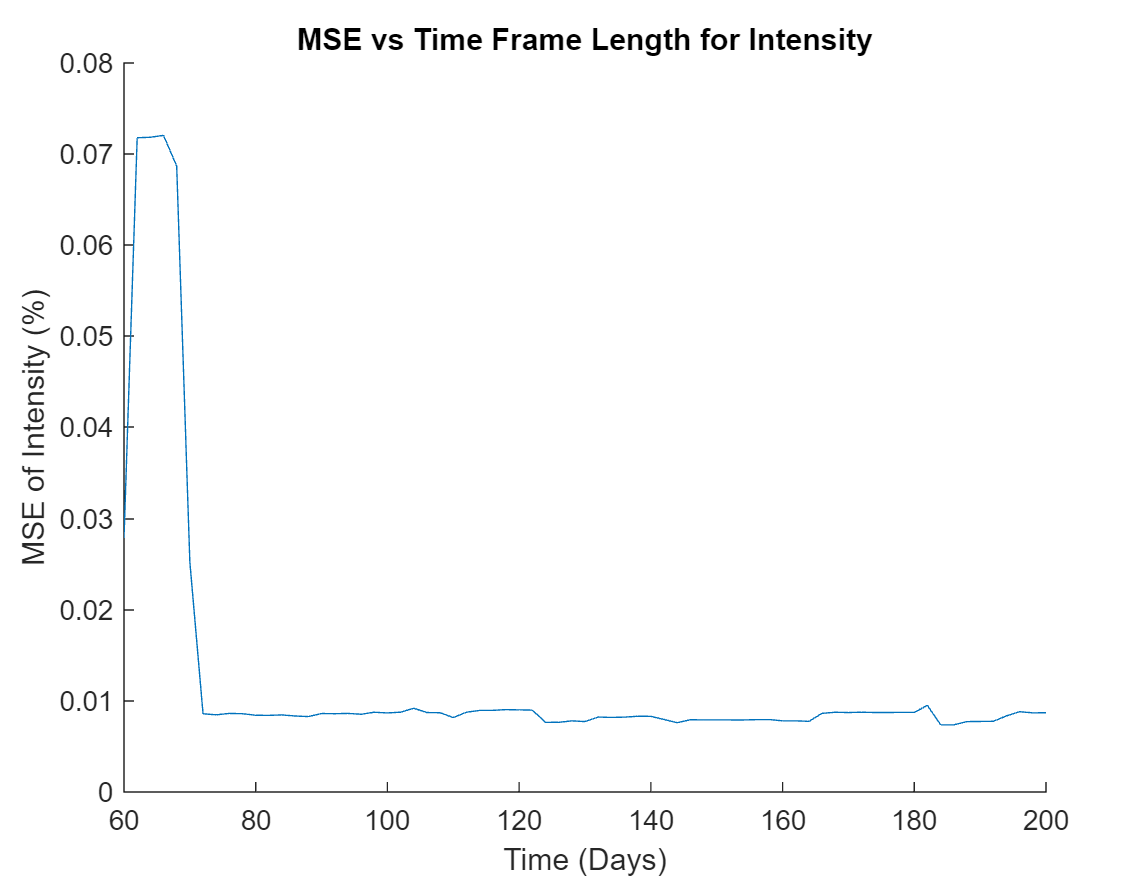
\includegraphics[width=140mm]{ActualVsPredValues/MSEvsStaticTimeFrame.png}
    \caption{The MSE over for intensity given different values of $t_f$. Note how the first minimum is not the global minimum within the context of this graph.}
    \label{fig:MSEStaticTimeFrame}
\end{figure}

Other than the obvious time complexity issues, a static time frame has other drawbacks that are more pertinent to the models behavior. In essence, the algorithm in listing \ref{lst:StaticTimeFrameFormula} will find the time frame that minimizes error across all time values greater than the target time. This results in the model finding a value for $t_f$ that minimizes error for all times greater than $t_t$, measuring accuracy in terms of the models \textit{global accuracy}. However, measuring accuracy this way violates the models efforts to adapt to the lifters current abilities. A static time frame may fail to capture changes, especially if changes are abrupt, or it may adapt to slowly, especially if the time frame is to long. If the lifters abilities change over time, then so to should the length of the time frame, thereby allowing changes in a lifters abilities to be more easily expressed.

\section{Choosing A Time Frame: Dynamic Time Frame Analysis}
\label{sec:TimeFrameDynamicTimeFrameAnalysis}

If the length of the time frame is allowed to vary over time it will give the model more freedom to adapt to the lifters current abilities. Much of the setup will remain the same from section \ref{sec:TimeFrameStaticTimeFrameAnalysis}, with equation \ref{eq:ValidTimeFrameSet} remaining valid in this section.  Figure \ref{fig:DynamicTimeFrameDiagram} demonstrates the process of selecting a dynamic time frame.

The algorithm to find a dynamic time frame is shown in listing \ref{lst:DynamicTimeFrameFormula}. The general idea of the algorithm is to select a time frame that minimizes the error of the closest data before the target time, and then that time frame can be used to predict the intensity at the target time. The main difference between the static and dynamic algorithms is the dynamic algorithm only measures accuracy in terms of the target time, and not in terms of every time before the target time. This results in the dynamic algorithm using the square error (SE) instead of the MSE to calculate accuracy for each individual target time. Once the SE is found for each target time the MSE can then be found across all target times. In essence, the dynamic time frame approach is only concerned with \textit{local accuracy}, whereas the static time frame approach is concerned with global accuracy.

\begin{figure}[h]
    \centering
    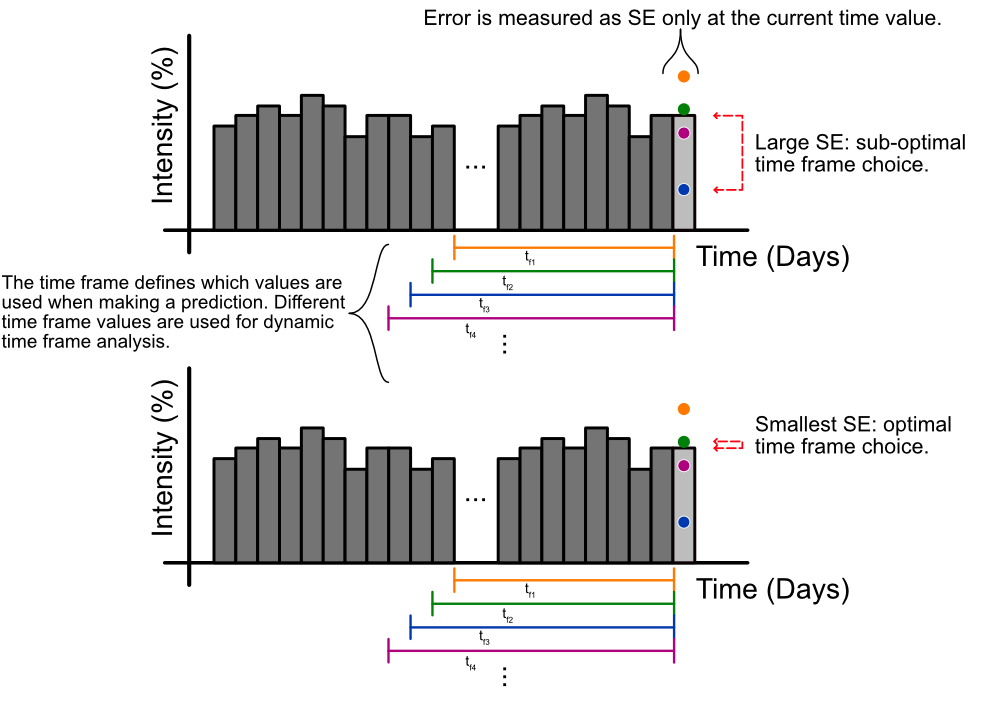
\includegraphics[width=150mm]{Diagrams/DynamicTimeFrameDiagram.png}
    \caption{A diagram showing how a dynamic time frame is calculated from the data set.}
    \label{fig:DynamicTimeFrameDiagram}
\end{figure}

A side effect of only measuring accuracy locally is an improved time complexity. The algorithm shown in listing \ref{lst:DynamicTimeFrameFormula} has a time complexity of $O(n^2)$, which is better than the $O(n^3)$ time complexity of the comparable static algorithm. This is also true for the algorithm to find historical data, with the dynamic algorithm shown in listing \ref{lst:HistoricalDynamicTimeFrameFormula} having a time complexity of $O(n^3)$. Obviously, these time complexities are still not great but it is a step in the right direction.

A dynamic programming approach similar to the one used in the static algorithm can also be used in listing \ref{lst:DynamicTimeFrameFormula} to reduce it's time complexity to $O(n)$. A linear time complexity is manageable, making the dynamic algorithm a viable way to select a time frame. This also reduces the time complexity of \ref{lst:HistoricalDynamicTimeFrameFormula} to be $O(n^2)$, which is not great, but can still be used to generate recent historical data.

Of course, only measuring accuracy locally does have some negative effects. Only measuring accuracy locally means that less information about the models performance is available when compared to the static algorithm. This is shown in the return values in listings \ref{lst:StaticTimeFrameFormula}-\ref{lst:HistoricalDynamicTimeFrameFormula}, with less information being returned from the dynamic algorithms. This is not a major concern however, as the accuracy of the model can still be assessed with the output of the dynamic algorithm.

\begin{minipage}{\linewidth}
\begin{lstlisting}[caption={The algorithm that describes how to exhaustively find a dynamic time frame's length such that it minimizes the models error.},label={lst:DynamicTimeFrameFormula},mathescape=true]
# $s$, $r$, $E$, $F$, and $t$ are all lists of there respective variables
fun dynamicTimeFrame$(s,r,E,F,t,t_t) \to \left( t_{f}, d_{iff} \right)$
    $t_{f,min}=0$
    $d_{iff,min}=\infty$
    $M_{min}=\{\}$
    for each $t_{f,i}\in \{ t_f \; | \; t_{t+1}+t_f\le \max_{t_1\dots t_n}(t) \} $
        # The $t+1$ subscript ensures the current data point, the value being
        # predicted, is not part of the model state
        $M=$modelState$(t_{t,i+1},t_{f,i})$
        $I_{pred}=$intesityPrediction$(M,s_{t+1},r_{t+1},E_{t+1},F_{t+1})$
        $d_{iff}=(I_{pred}-I_{t+1})^2$
        if $d_{iff}<d_{iff,min}$
            $\left( d_{iff,min}, t_{f,min}, M_{min} \right)=\left(  d_{iff}, t_{f,i}, M \right)$
    return $(t_{f,min},(\texttt{intensityPrediction}(M_{min},s_t,r_t,E_t,F_t)-I_t)^2)$
\end{lstlisting}
\end{minipage}

\begin{minipage}{\linewidth}
\begin{lstlisting}[caption={The algorithm that describes how to find historical dynamic time frames.},label={lst:HistoricalDynamicTimeFrameFormula},mathescape=true]
# $s$, $r$, $E$, $F$, and $t$ are all lists of there respective variables
fun historicalDynamicTimeFrames$(s,r,E,F,t) \to \left( [t_{f,1},\dots,t_{f,n}], \varepsilon \right)$
    $d_{iff}=[\infty, \infty, \dots]$ where $|d_{iff}|=|t|$
    $t_{f,min}=[0, 0, \dots]$ where $|t_{f,min}|=|t|$
    for each $t_{t,i}\in \{ t \}$
        $(t_{f,min}[i],d_{iff}[i])=$dynamicTimeFrame$(s,r,E,F,t,t_{t,i})$
    return $($
        $t_{f,min}$,
        $\texttt{sum}(
            \texttt{filter}(d_{iff},\texttt{val}!=\infty)
        )/
        \texttt{count}(
            \texttt{filter}(d_{iff},\texttt{val}!=\infty
        )$
    $)$
\end{lstlisting}
\end{minipage}

Figure \ref{fig:PredictionsVsActualDynamicTimeFrame} is the result of running the dynamic time frame algorithm on deadlift data. Note how the MSE has decreased to $0.42\%$ compared to $0.78\%$ from the static algorithm. Put another way: using a dynamic time frame the model is, on average, within $0.42\%$ of the actual intensity. Other than the increased accuracy, another thing of note is the increased range over which predictions were able to be made compared to the static time frame shown in table \ref{tab:PredictionsVsActualConstantTimeFrame}. This is because the models time frame was able to shrink when it butted up against the end of the data set in the dynamic approach, whereas in the static approach if the time frame went past the end of the data set no predictions could be made.
%and figure \ref{fig:TimeFrameAcrossTime} shows the time frame length across time

\begin{figure}[h]
    \centering
    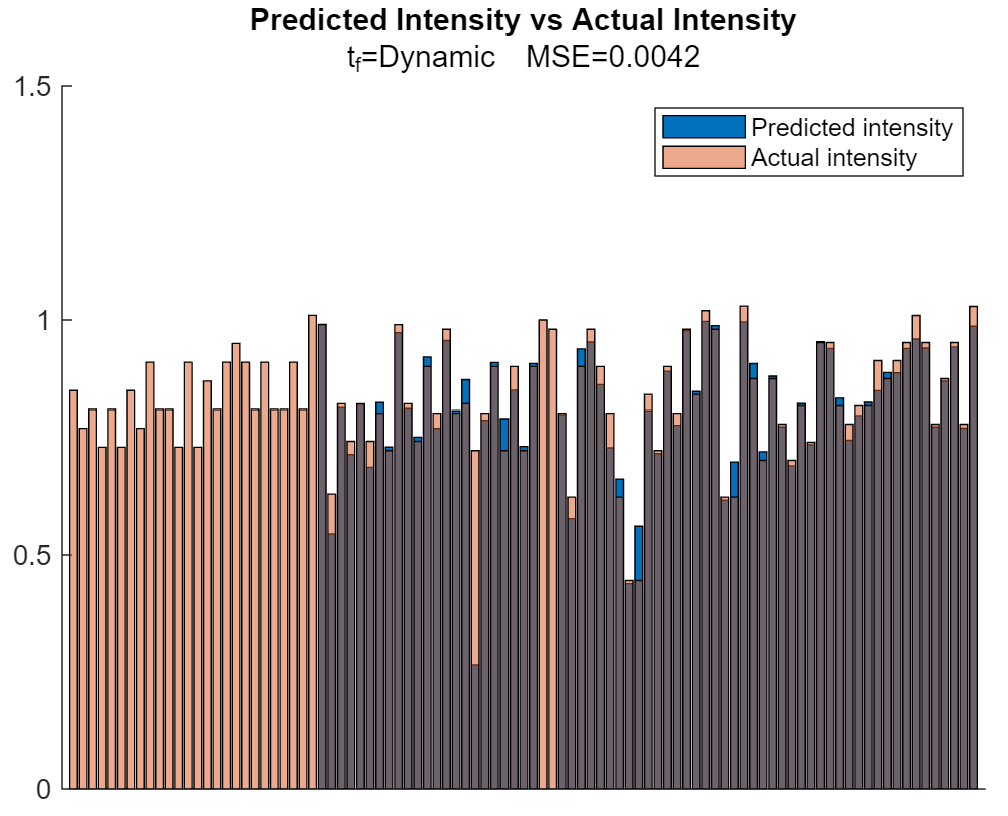
\includegraphics[width=120mm]{ActualVsPredValues/DynamicTimeFrameActualVsPredIntensity.png}
    \caption{Predicted values compared to actual values for intensity using deadlift data. Note how using the dynamic time frame extended the range of values that have predictions while still having higher accuracy.}
    \label{fig:PredictionsVsActualDynamicTimeFrame}
\end{figure}
%\begin{figure}[h]
%    \centering
%    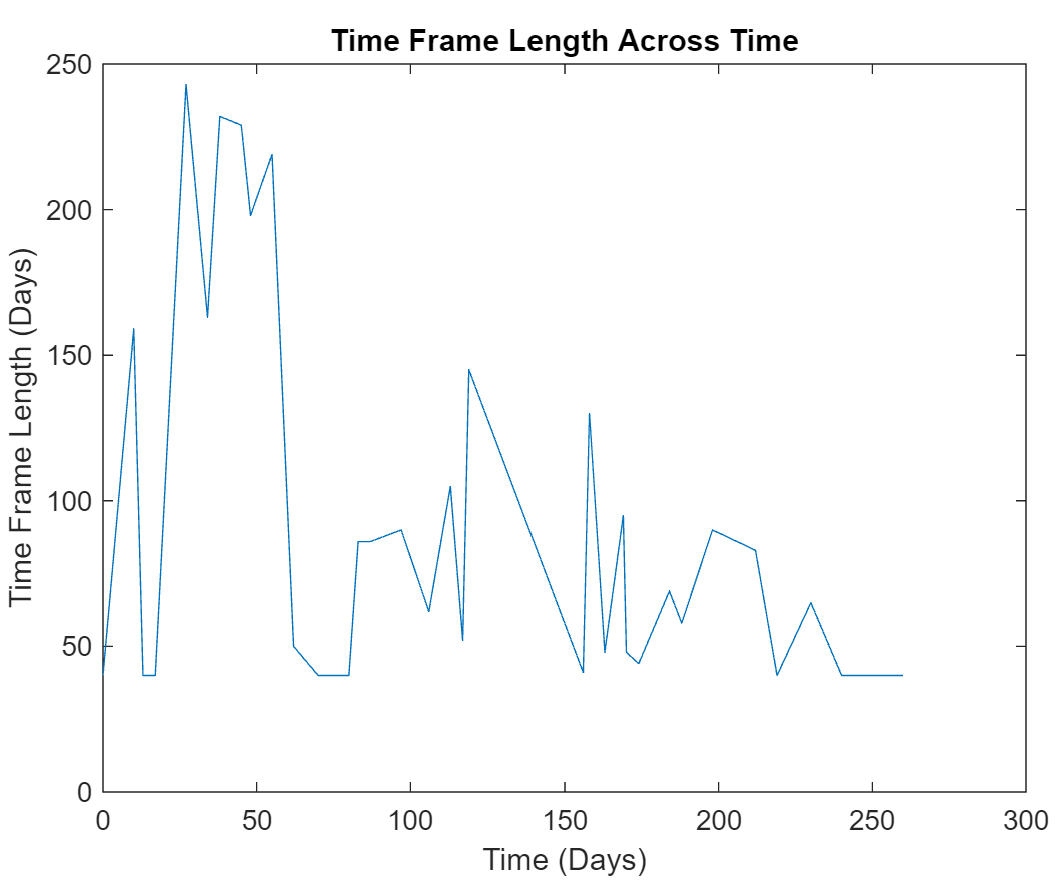
\includegraphics[width=120mm]{DeadliftConstants/TimeFrameLengthAcrossTime.png}
%    \caption{Time frame length over time. Note the general trend of increasing time frames, which is partly a function of the model having more data to work with as $t_t\to 0$.}
%    \label{fig:TimeFrameAcrossTime}
%\end{figure}

%TODO - add plot showing updated 1RM predictions

\section{Choosing A Time Frame: The General Case Through Sliding Window Analysis}
\label{sec:TimeFrameSlidingWindowAnalysis}

It turns out that the two 

\section{Analysis: Injuries, Setbacks, and Changes}
\label{sec:TimeFrameInjuriesAndChanges}

Section \ref{sec:TimeFrameDynamicTimeFrameAnalysis} was concerned with allowing the model to better adapt to a lifters current abilities. Using a 'local' measure of accuracy seemed to allow this, but proof that it does is needed.

An obvious place to check if the model is adapting to the lifters current abilities is the dates surrounding the lifters injury on $3/3/2022$. After an injury the model should respond by reducing the time frame so that only recent data is included, reflecting any drop in performance. A second place to check where the model adapts to a lifters current abilities is the dates surrounding any 1RM attempt. If the lifter peaked properly for the attempt then the models time frame should decrease leading up to the attempt and then re-increase again afterwards.

Looking at the time frame from $3/27/2022$-$5/30/2022$ the aforementioned patterns are present. The relevant data points and there respective time frames shown in table \ref{tab:TimeFrameNearCompetitionDeadlift}. From $3/27/2022$-$4/9/2022$ the time frame is trending downwards, indicating the model is adapting to the lifters post-injury capabilities. From $4/9/2022$-$4/28/2022$ the time frame re-increases, indicating the lifters abilities are returning. From $4/28/2022$-$5/5/2022$ the time frame decreases as the lifter approaches the competition on $5/5/2022$. Then, after the competition the time frame increases again. The behaviors of the time frame from table \ref{tab:TimeFrameNearCompetitionDeadlift} show the model is adapting to the lifters current abilities.

%An example of this is from the deadlift data between the dates of $4/2/2022$ and $5/30/2022$. The relevant data points and there respective time frames shown in table \ref{tab:TimeFrameNearCompetitionDeadlift}. Notice how as the competition approaches the models time frame begins to decrease, and afterwards the time frame re-increases. This is because the model was picking up on the lifters peak leading into the competition, where performance is temporarily boosted due to decreased fatigue levels.

\begin{table}[h]
    \centering
    \begin{tabular}{c|c}
        Date & $t_f$ \\
        \hline
        $3/27/2022$ & $145$ \\
        $3/29/2022$ & $52$ \\
        $4/2/2022$ & $105$ \\
        $4/9/2022$ & $62$ \\
        $4/18/2022$ & $90$ \\
        $4/28/2022$ & $86$ \\
        $5/2/2022$ & $86$ \\
        $5/5/2022$ & $40$ \\
        $5/15/2022$ & $40$ \\
        $5/23/2022$ & $50$ \\
        $5/30/2022$ & $219$
    \end{tabular}
    \caption{Time frame length over time when a lifter was peaking for a competition on $5/5/2022$. Notice how the time frame decreases as the competition approaches and then re-increases. This is proof the model can capture recent changes in training.}
    \label{tab:TimeFrameNearCompetitionDeadlift}
\end{table}

If an injury is severe enough, a lifter may loose all training progress and may never be capable of the same performance ever again. The data set (thankfully) does not have any data relating to a case like this, which makes it difficult to assess how quickly the model would respond to such a scenario. Even if the model does not respond quickly however, it does not make sense to include any data from the time before the injury occurred. To ensure this does not happen, the time frame can be limited to only include data from after the injury, creating a clean slate for the model to re-learn the lifters new abilities.

\section{Application: Predicting the Future?}
\label{sec:TimeFramePredictingTheFuture}

Up until now, the model was only making predictions about the current day. The next natural question is can the model make predictions further in the future? The answer is yes, but only based on the models current state. This is a pretty big 'but', as the models state will have changed by the time any future date is reached, thereby changing any predictions it would have made. To further complicate the issue, the more data is added to the data set between the current time and the predicted time the greater the potential is for the model state to vary drastically. This generally means the further out a prediction is in the future the less accurate it will be, and it is this reason that the predictions have been limited to only capture the next training session, and not reach beyond that. However, if changes to the models state can be predicted over time, then more valid predictions can be made about the future.

%TODO - make plot showing how this happens

%The next chapter will deal with finding patterns in the changing of state - a meta analysis
\section{
    Macrocycle
    \\
    \large{A Meta-Analysis}
}
\label{sec:Macrocycle}

%The previous section established what is possible for a lifter. This removed uncertainly about what could be done, however it must still be decided exactly what a lifter should do over the course of a training cycle to maximize results.

%TODO - introduce plots over time here
%\include{Mesocycle}

\appendix

\section{
    Appendix A
    \\
    \large{Potential Surface Graphs for Squat, Bench, and Deadlift}
}
\label{sec:AppendixA}

\begin{table}[h]
    \centering
    \begin{tabular}{c|c}
        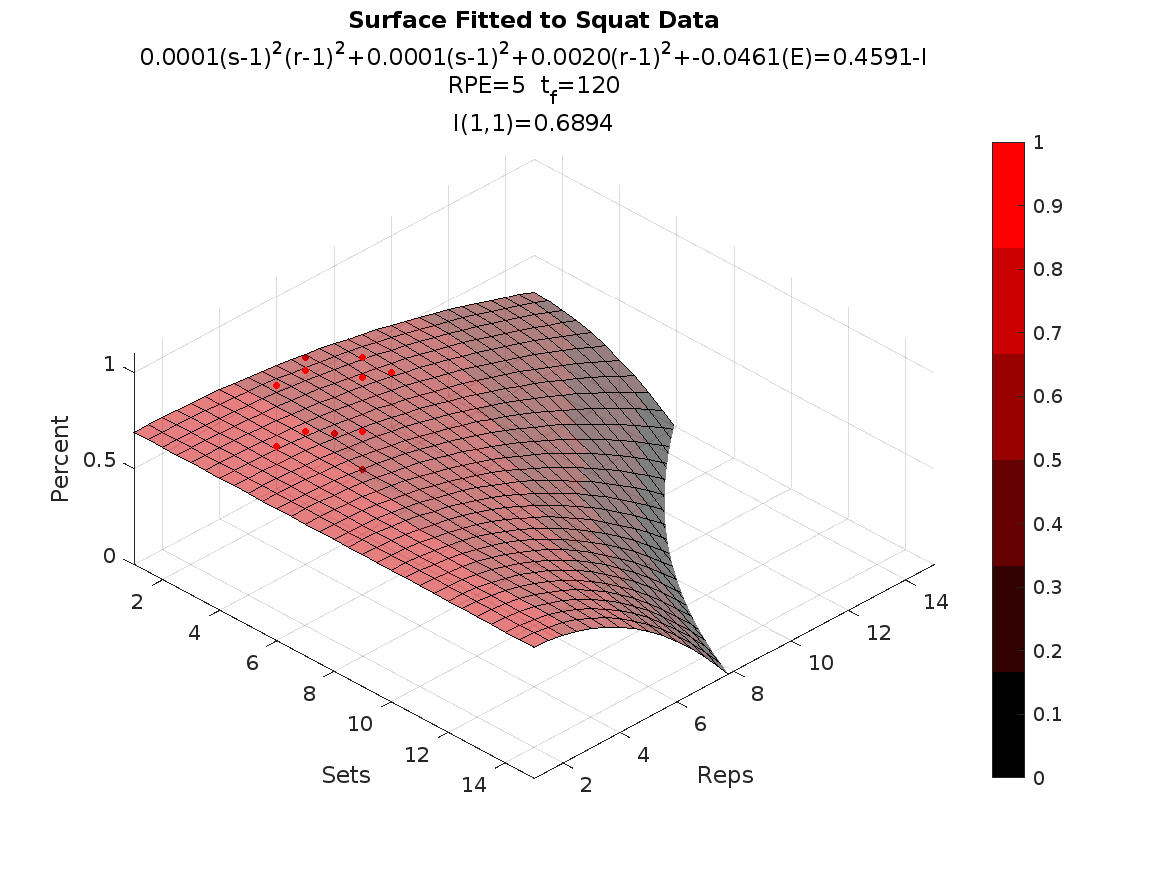
\includegraphics[width=78mm]{SquatSurface/5.png} &  
        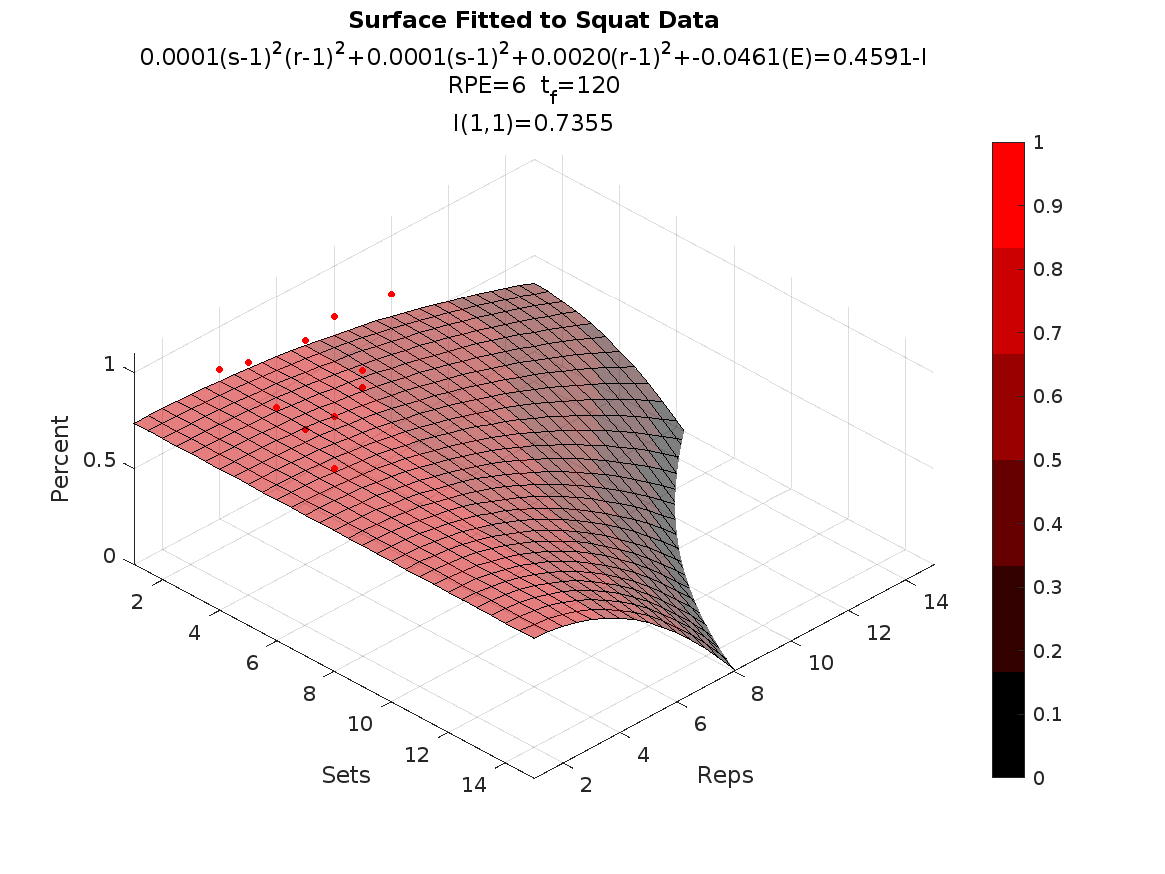
\includegraphics[width=78mm]{SquatSurface/6.png} \\
         
        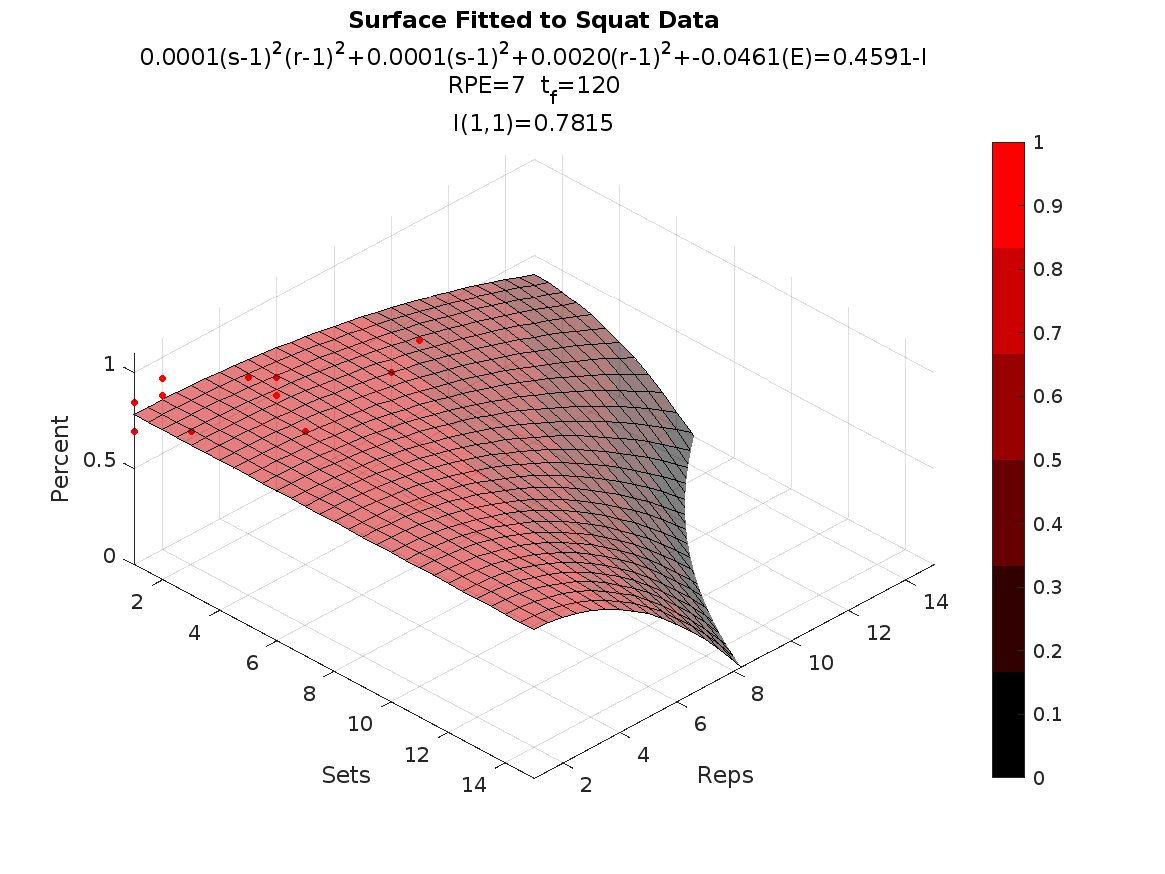
\includegraphics[width=78mm]{SquatSurface/7.png} &
        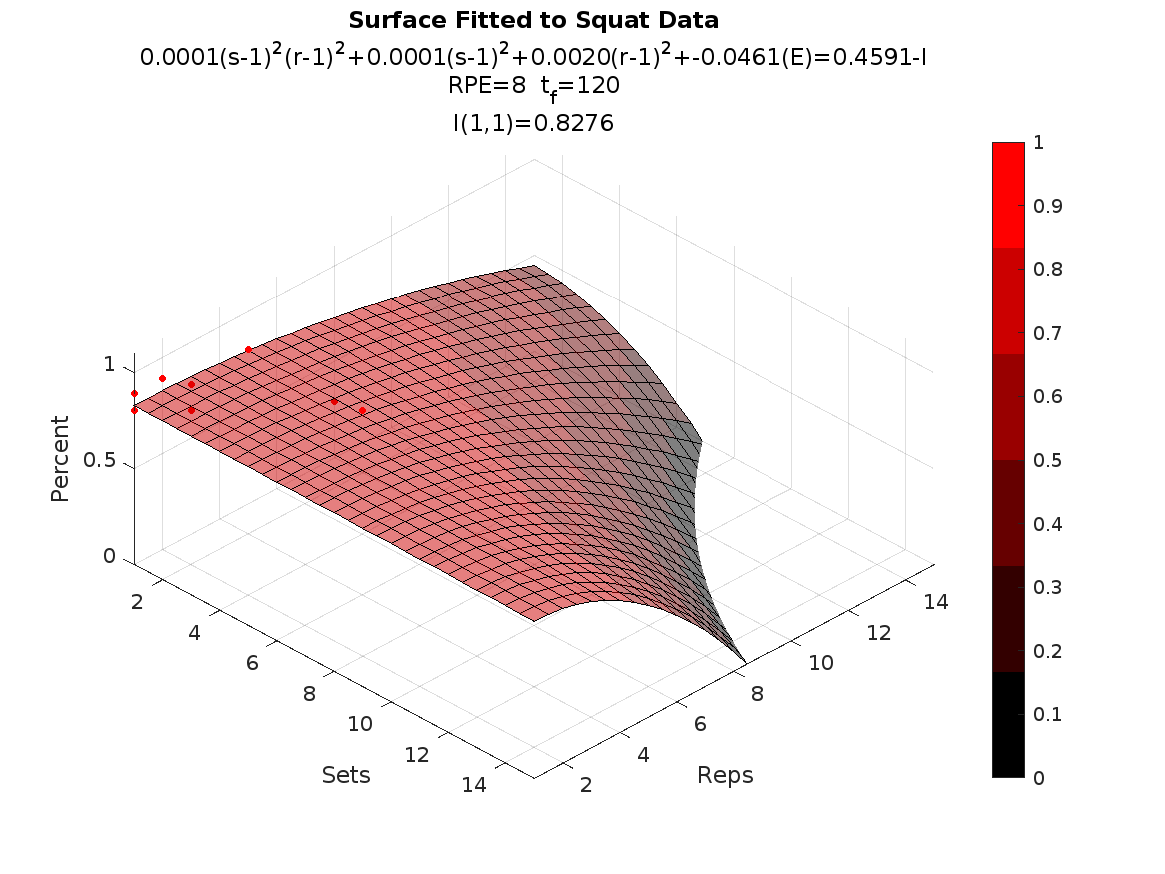
\includegraphics[width=78mm]{SquatSurface/8.png} \\
        
        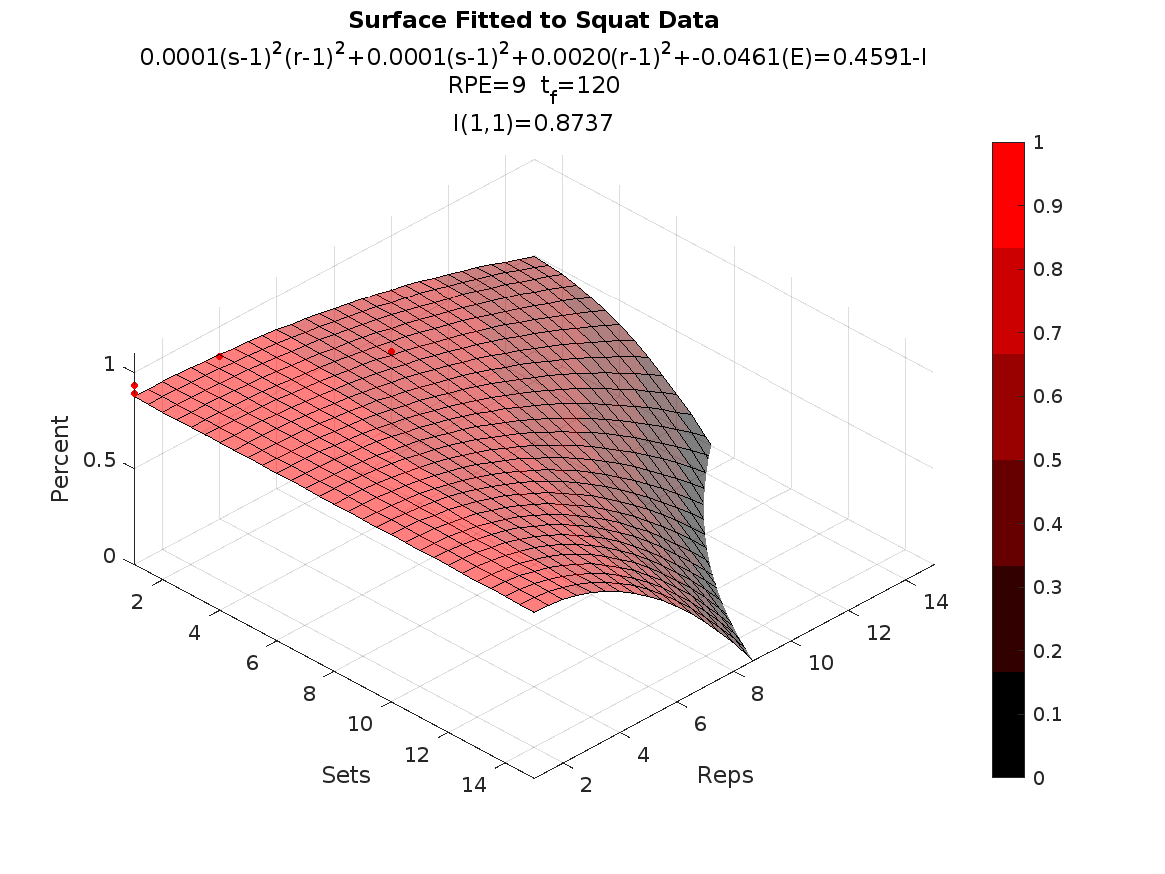
\includegraphics[width=78mm]{SquatSurface/9.png} &
        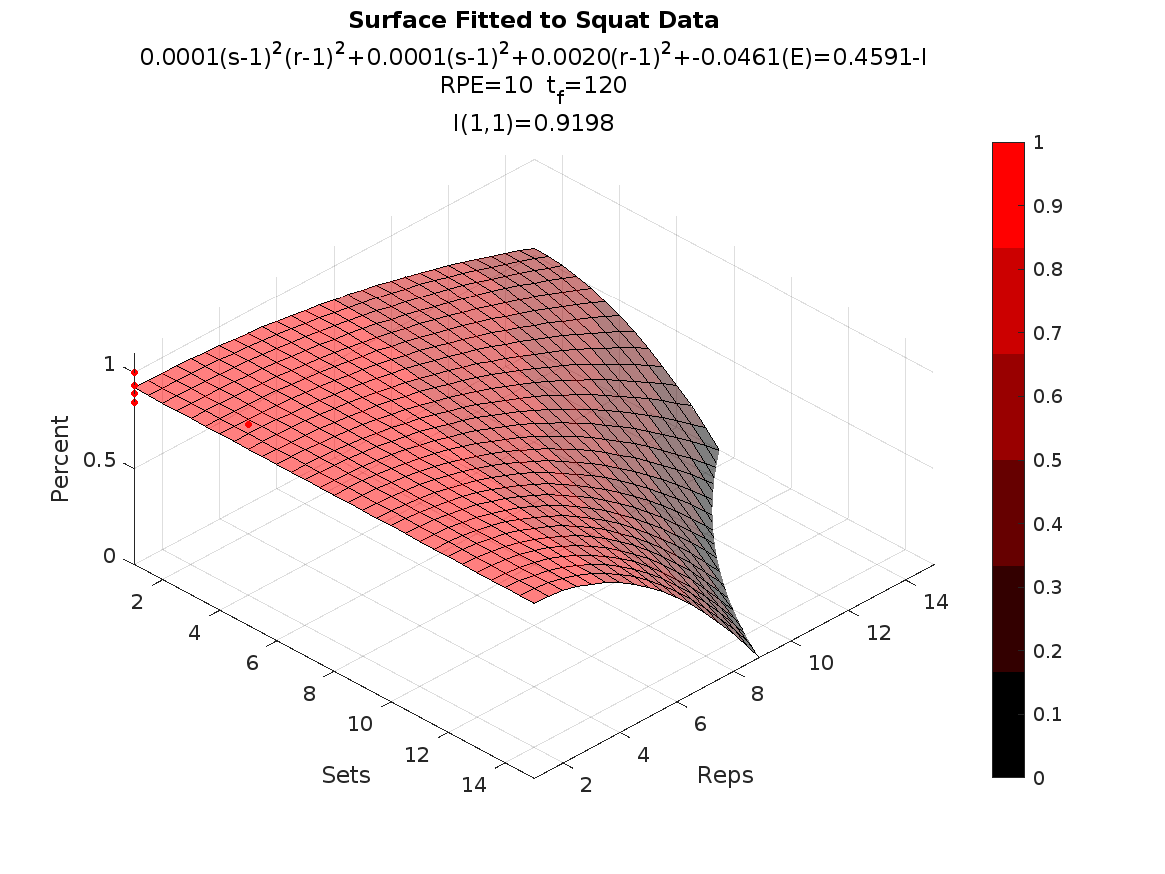
\includegraphics[width=78mm]{SquatSurface/10.png} \\
    \end{tabular}
    \caption{The potential surface fitted to squat data at various effort levels.}
    \label{tab:AppBSquatPotentialSurfaceAcrossEffort}
\end{table}

\begin{table}[h]
    \centering
    \begin{tabular}{c|c}
        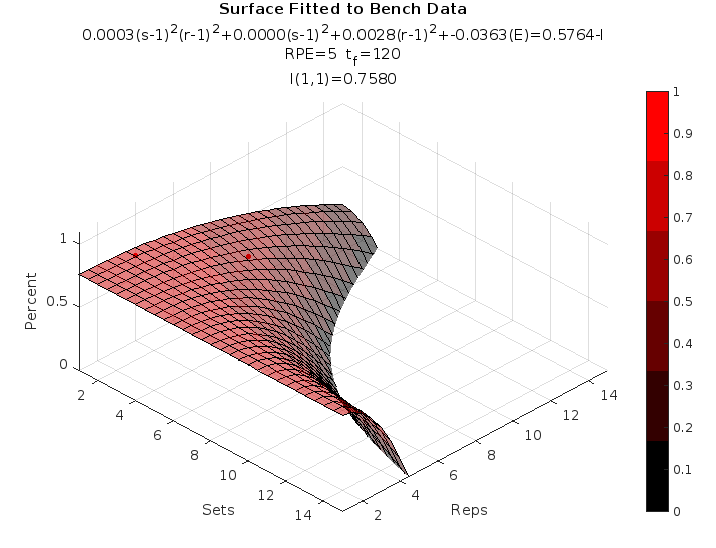
\includegraphics[width=80mm]{BenchSurface/5.png} &  
        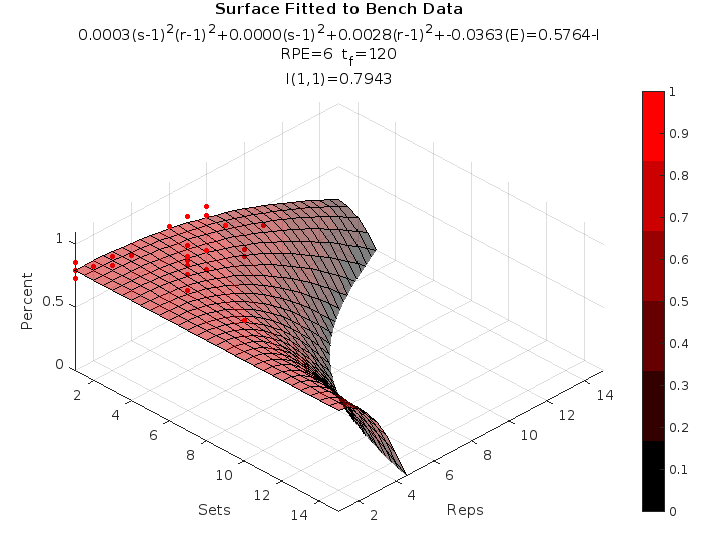
\includegraphics[width=80mm]{BenchSurface/6.png} \\
         
        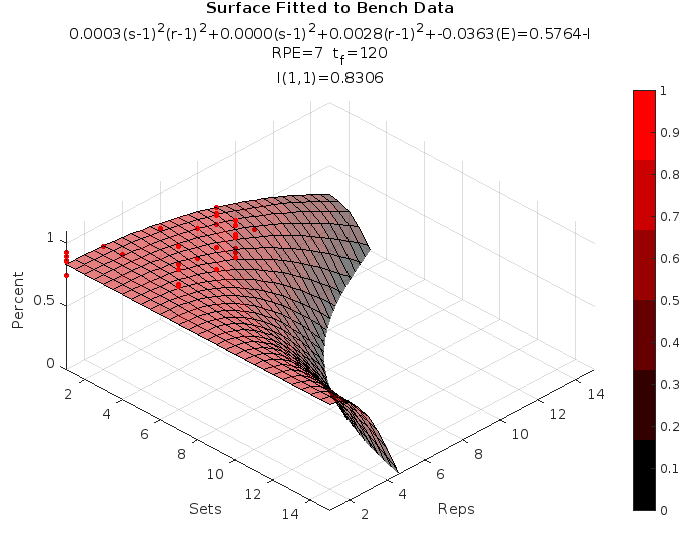
\includegraphics[width=80mm]{BenchSurface/7.png} &
        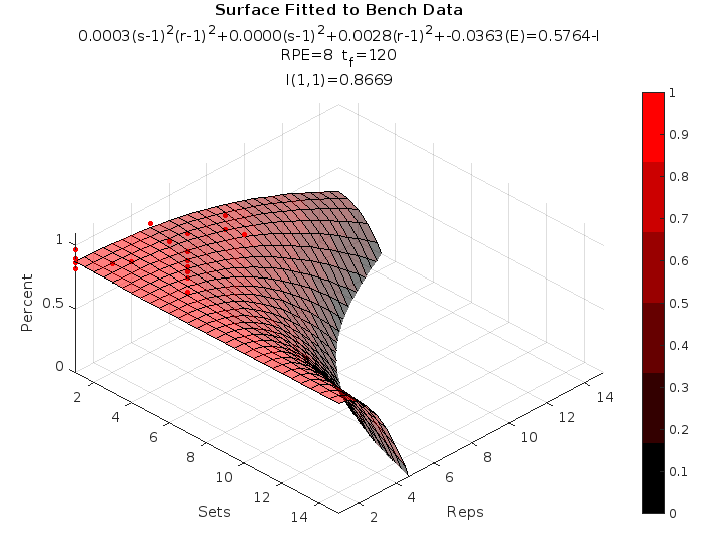
\includegraphics[width=80mm]{BenchSurface/8.png} \\
        
        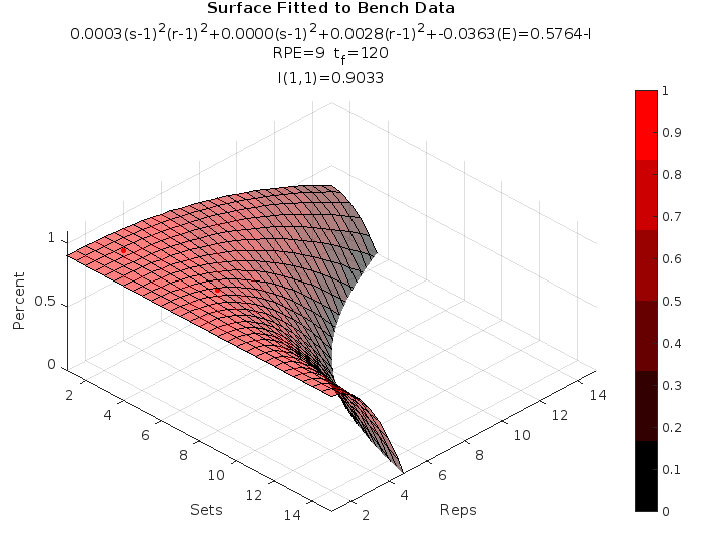
\includegraphics[width=80mm]{BenchSurface/9.png} &
        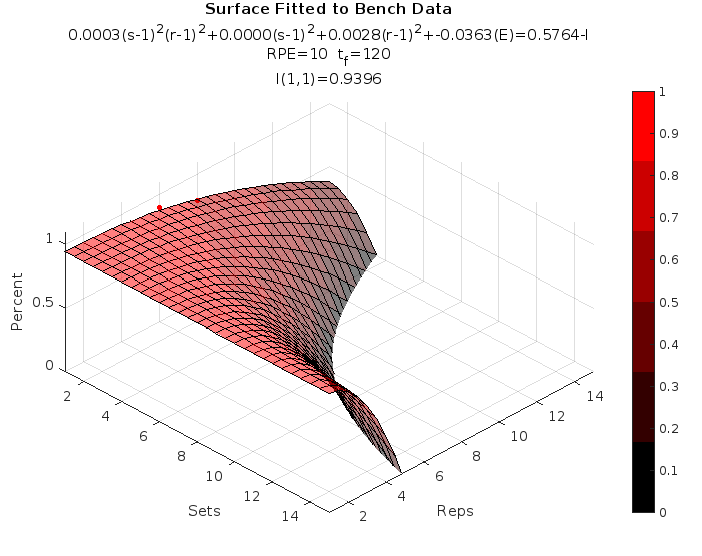
\includegraphics[width=80mm]{BenchSurface/10.png} \\
    \end{tabular}
    \caption{The potential surface fitted to bench data at various effort levels.}
    \label{tab:AppBBenchPotentialSurfaceAcrossEffort}
\end{table}

\begin{table}[h]
    \centering
    \begin{tabular}{c|c}
        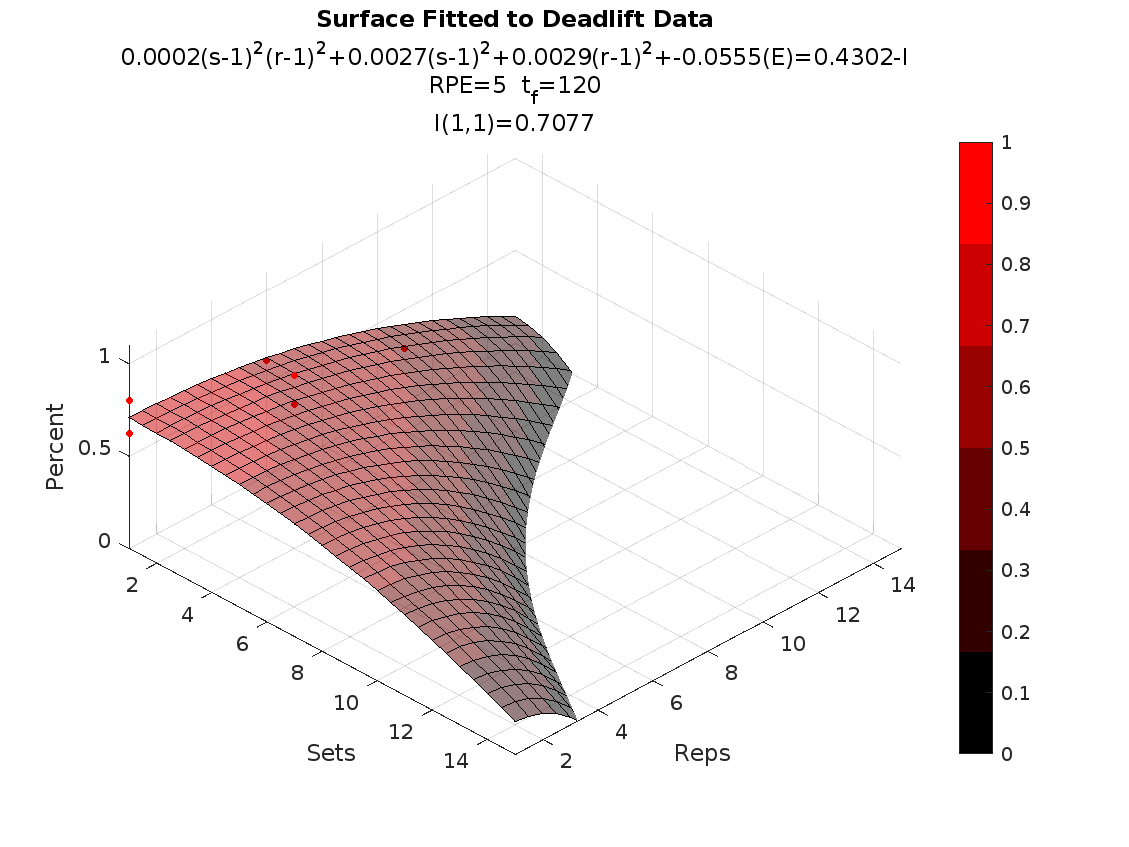
\includegraphics[width=80mm]{DeadliftSurface/5.png} &  
        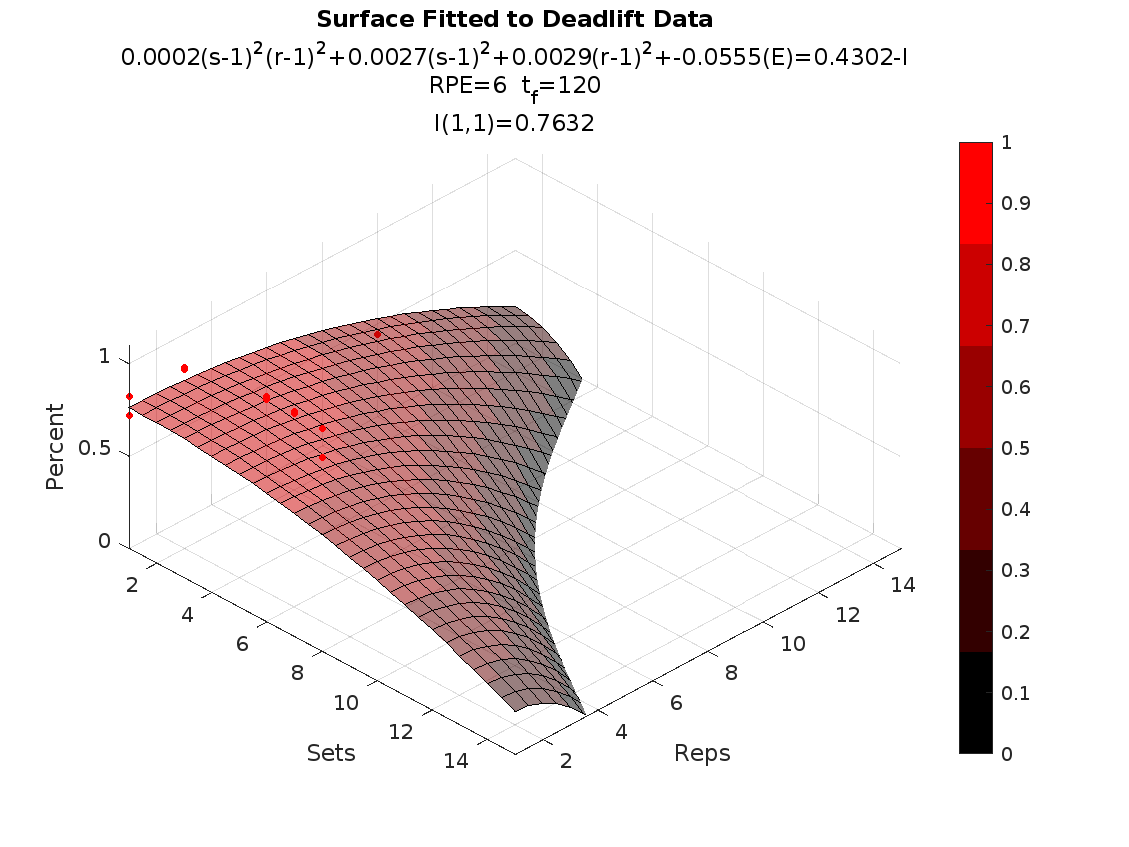
\includegraphics[width=80mm]{DeadliftSurface/6.png} \\
         
        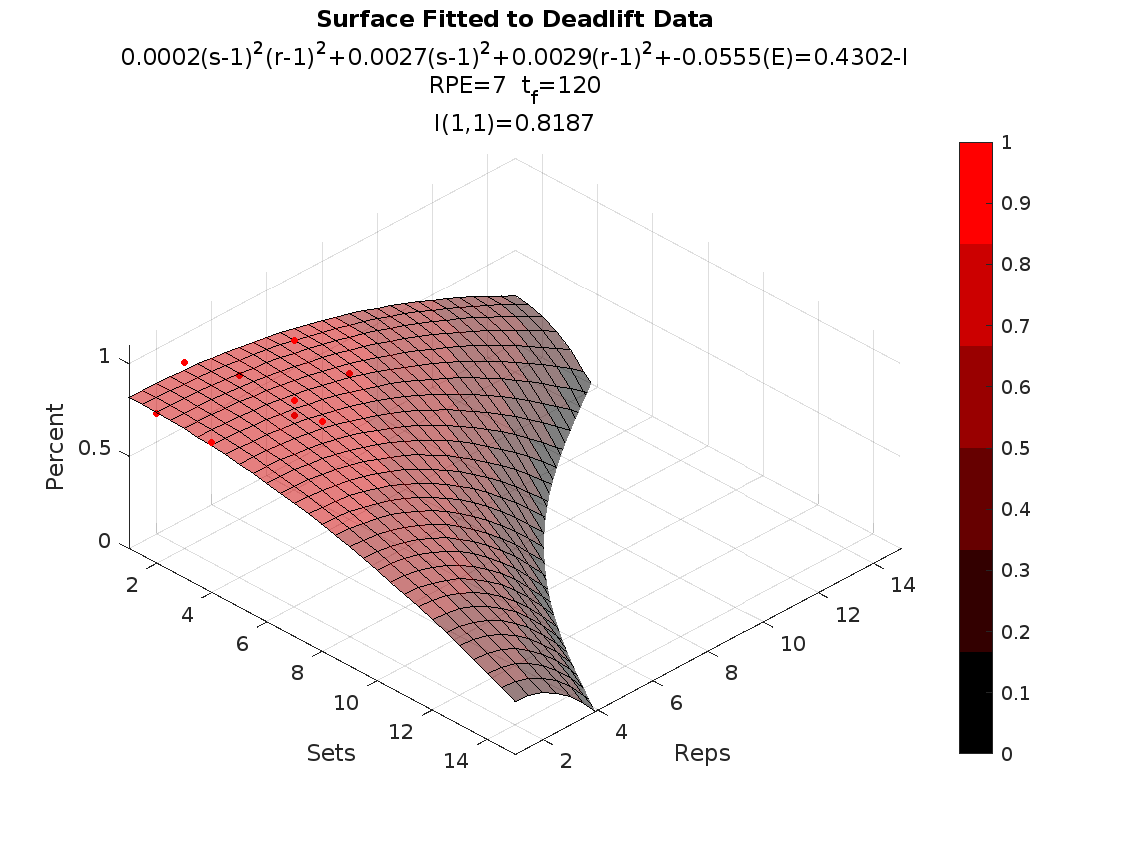
\includegraphics[width=80mm]{DeadliftSurface/7.png} &
        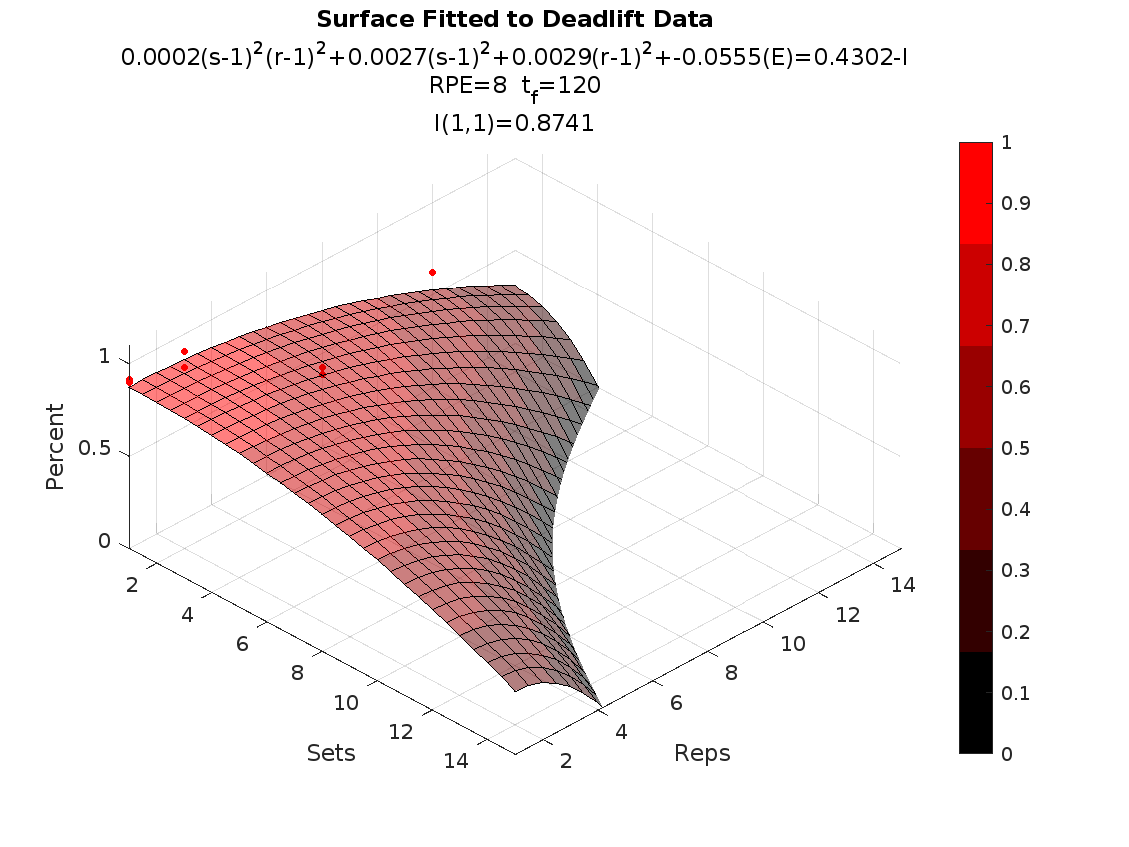
\includegraphics[width=80mm]{DeadliftSurface/8.png} \\
        
        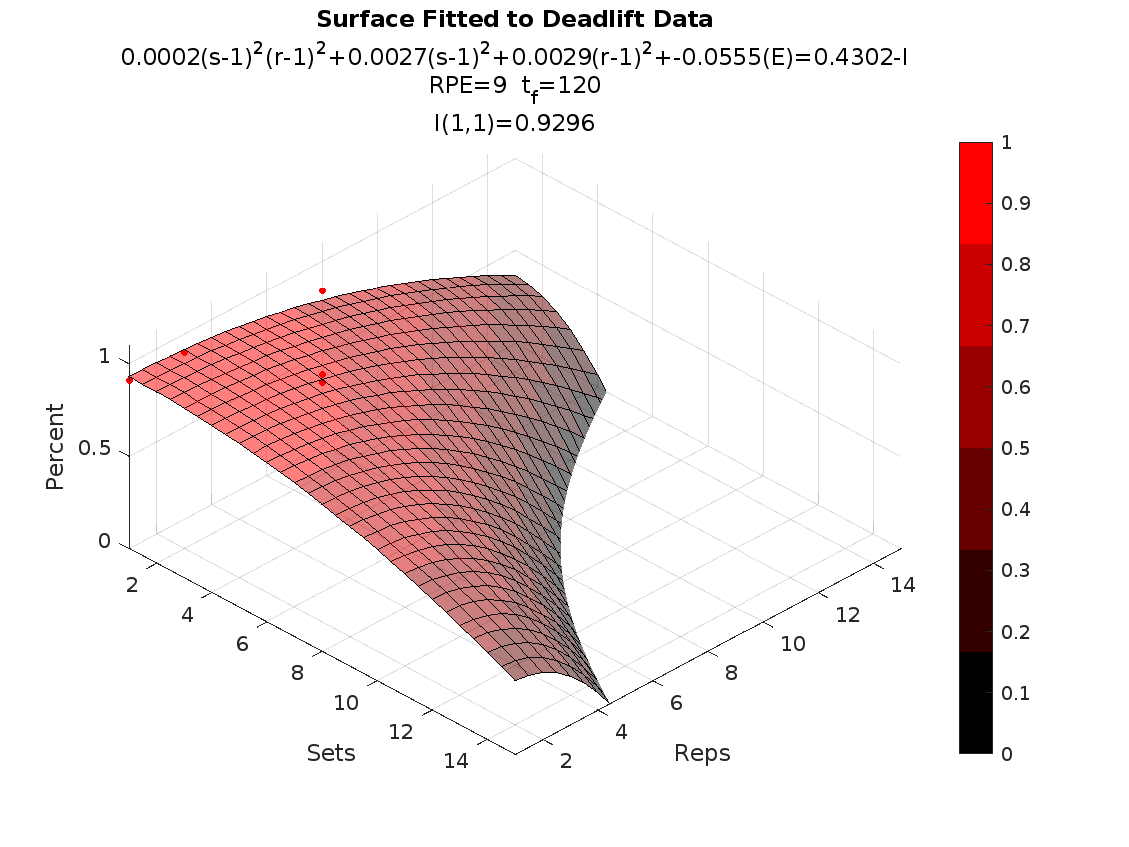
\includegraphics[width=80mm]{DeadliftSurface/9.png} &
        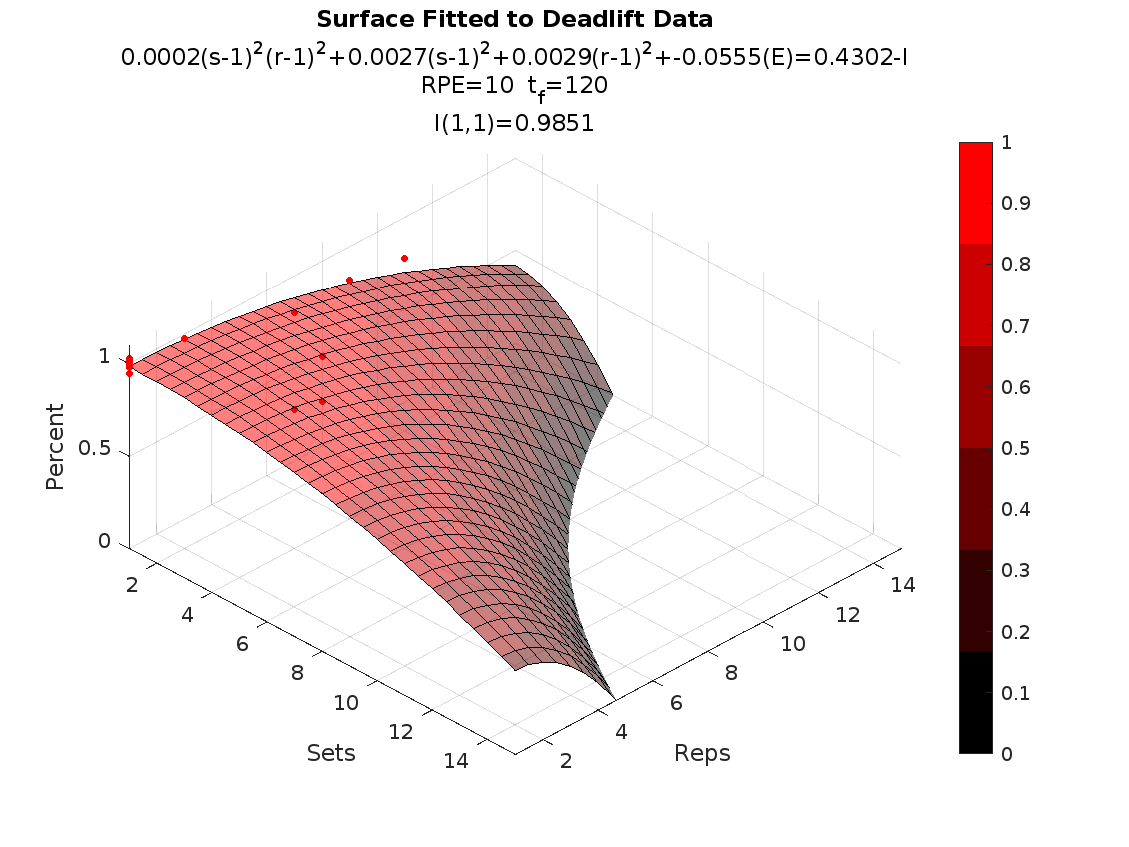
\includegraphics[width=80mm]{DeadliftSurface/10.png} \\
    \end{tabular}
    \caption{The potential surface fitted to deadlift data at various effort levels.}
    \label{tab:AppBDeadliftPotentialSurfaceAcrossEffort}
\end{table}

\printbibliography[heading=bibintoc,title={References}]

\end{document}